\begin{abstract}
Language models are increasingly asked for advice about financial positions
people already hold, and they carry measurable behavioural bias. Whether
deliberation removes it is unsettled, because the available evidence either
compares different models, so that capability and deliberation move together,
or infers deliberation from the model's own account of its reasoning,
produced by the same forward pass as the answer. We instead set the
reasoning budget exogenously through the API, at three levels, before the
model sees the item, and measure nine families of normatively irrelevant cue
against matched pairs that differ only in that cue. Across 9{,}720 responses
from three models the disposition effect runs opposite to the human
direction: pooled, these models are more willing to sell at a loss than at a
gain, $+0.239$ $[+0.148, +0.331]$ on the categorical measure and $+13.4$
$[+8.8, +18.0]$ percentage points of the position, where the pre-registered
prediction was negative, though the reversal is carried by the two smaller
models and appears in the strongest only as effort rises. Reasoning effort reduces the absolute effect in all
nine qualifying cases, against a shuffled-label null of 0.0125 rather than
the $2^{-9}$ a count would suggest, and it does so by compressing the spread
of bias magnitudes across families: the mean falls detectably in the
strongest model alone, and the compression itself is robust in the weakest,
where no shuffle in 2{,}000 reproduces it, and inseparable from sampling
error in the strongest. The exogenous manipulation is what makes this
visible. Measured the observational way on the same responses, with output
tokens standing in for displayed deliberation, more reasoning goes with
\textit{more} bias between items and with nothing at all within an item. We
also report that \texttt{temperature} is unavailable on these models, which
makes the fixed-temperature protocol used throughout this literature
unexecutable, and give a repeated-sampling replacement.
\end{abstract}

\section{Introduction}
\label{sec:intro}
Language models now sit inside the tools through which ordinary people make
financial decisions, and are increasingly asked not for a price or a
definition but for a recommendation about a position someone already holds.
That they carry measurable behavioural bias is the premise here rather than
the finding: human dual-process failures reproduce in them
\citep{hagendorff2023intuitive}, thirty biases appear across twenty models
\citep{malberg2025comprehensive}, and preference-based responses grow less
rational as models advance \citep{bini2026behavioral}.

Whether deliberation removes any of it is unsettled. Reasoning models are
less prone to anchoring \citep{takenami2025anchoring} but no better protected
in clinical vignettes \citep{kim2025biasmedqa}; the effort parameter has been
reported to set a ceiling on generation rather than to drive how reasoning is
allocated \citep{hu2026effort}; and an indicator for analytical reasoning
raises rational responses by 40\% \citep{bini2026behavioral}. Each either
compares different models, so that capability and deliberation move together,
or measures something other than a decision, or relies on the model's own
account of its reasoning. The reasoning budget has not been
manipulated as a treatment against a behavioural finance bias. That is this
paper.

Across 9{,}720 responses the disposition effect runs opposite to the human
direction, reasoning effort reduces the absolute effect in all nine cases
that qualified for the pre-registered test, and within a fixed effort level
the association between generated length and bias is positive rather than
negative.

\ifsubmission
The 40\% figure of \citet{bini2026behavioral} is the sharpest case. Their
indicator is the model's own characterisation of its reasoning, emitted in
the same response as the answer it describes, so a model that answers well
and then calls its own reasoning analytical produces the association with no
causal path from deliberation to accuracy. A budget set before the model sees
the item is independent of what it goes on to say, and the distinction can be
measured here rather than argued, because the data holds both variables.
Section~\ref{sec:mediator} substitutes the tokens the model chose for the
budget the experimenter set, on the same responses, and the answer changes
sign.
\else
The identification problem in prior work is worth stating precisely.
\citet{bini2026behavioral} report that an indicator for self-reported
analytical reasoning raises the share of rational responses by roughly 40
percent, and treat that indicator as a mediator for the effect of role
priming. The indicator is the model's own characterisation of its reasoning,
emitted in the same response as the answer it describes. A model that answers
well and then calls its own reasoning analytical produces that association
with no causal path from deliberation to accuracy. The reasoning budget, by
contrast, is set before the model sees the item and is independent of what it
goes on to say, which is what makes the comparison reported here an
experiment rather than an association.

That distinction is usually left as an argument. Here it can be measured,
because the data holds both kinds of variable: the budget the experimenter
set, and the tokens the model chose to spend. Section~\ref{sec:mediator}
runs the paper's own analysis on the same responses with the second in place
of the first, and the answer changes sign. The design is not a refinement of
the observational one; on this data it is the difference between finding the
effect and finding its opposite.
\fi

Our contributions are:
\begin{itemize}
  \item The first measurement, to our knowledge, of behavioural finance bias
        under an exogenous, graded manipulation of reasoning effort.
  \item A matched pair battery of nine biases in advisory framing with
        realistic portfolio state, two of them absent from prior work,
        released in full.
  \item A distributional protocol, forced by the removal of sampling
        parameters from the API: repeated sampling and bootstrap intervals in
        place of single deterministic draws, with within-item entropy
        reported as a result.
  \item A test of what the exogeneity buys. Substituting an endogenous
        measure of displayed reasoning for the manipulated budget, on the
        same responses, reverses the sign.
  \item A pre-registered plan committed before the first API call, with the
        prompts, raw responses and analysis code.
\end{itemize}

\section{Related Work}
% ~1 page, three subsections. Every paragraph ends on why that work does not
% answer this question. LITERATURE.md has the full search record. Of the four
% items it listed as unread, three are now closed: Bini Table 1 and Malberg
% B.30 were read in full on 2026-10-26 and the SSRN sweep was run. Two full
% texts remain unobtainable, piya2026overthinking behind SSRN bot detection
% and chon2025variability behind a paywall, and no finding of either is
% relied on here.

\subsection{Behavioural biases in human investors}
\label{sec:humaninvestors}
\ifsubmission
The biases tested here are documented regularities in human investors and the
design borrows their operationalisations rather than inventing new ones:
prospect theory \citep{kahneman1979prospect} and framing
\citep{tversky1981framing}, the disposition effect
\citep{shefrin1985disposition} as measured in brokerage data by
\citet{odean1998losses}, mental accounting \citep{thaler1985mental}, myopic
loss aversion \citep{benartzi1995myopic} and home bias
\citep{french1991homebias}. \citet{barber2000hazardous} supply the reason to
measure them in an advisor at all: they cost realised returns.
Appendix~\ref{app:humaninvestors} maps each finding to the family built from
it, and the human baselines of Appendix~\ref{app:humanbaselines} are
indicative rather than like for like.
\else
\movedhead{Behavioural biases in human investors}
\label{app:humaninvestors}
The biases this paper tests are not hypotheses about language models. They
are documented regularities in human investors, and the design borrows their
operationalisations rather than inventing new ones. Prospect theory
\citep{kahneman1979prospect} supplies the reference dependence that makes a
cost basis matter at all, and the framing manipulations of
\citet{tversky1981framing} supply the form of the framing family here: the
same information, valenced two ways. The disposition effect was named by
\citet{shefrin1985disposition} as a reluctance to realise losses and measured
in brokerage account data by \citet{odean1998losses}, who scores which
positions investors sell when they sell something. Mental accounting
\citep{thaler1985mental} motivates the sleeve manipulation, myopic loss
aversion \citep{benartzi1995myopic} the evaluation horizon, and home bias
\citep{french1991homebias} the domestic and foreign arms.
\citet{barber2000hazardous} supply the reason any of this is worth
measuring in an advisor: these biases carry a cost in realised returns.

These are also the source of the human baselines in
Section~\ref{sec:humanbaselines}, and the comparison is indicative rather
than like for like, because a field study of brokerage accounts and a
prompt battery are different instruments.
% Closed 2026-10-26. The Odean rates in Section 4.2 are read from Table I on
% p.1783 of the primary paper, not from any summary of it. Any further human
% rate added later must clear the same bar.

\fi

\subsection{Behavioural bias in language models}
\ifsubmission
That language models exhibit behavioural biases is established, and this
paper does not re-establish it. Models have served as experimental subjects
for cognitive tasks \citep{binz2023cognitive, hagendorff2023intuitive}, as
simulated economic agents \citep{horton2023homosilicus} and as stand-ins for
survey populations \citep{argyle2023silicon, aher2023simulating}. Three
audits set the state of the art: thirty biases across twenty models
\citep{malberg2025comprehensive}, sixteen cognitive-psychology questions
across twelve models \citep{bini2026behavioral}, and eight behavioural
parameters over 24{,}000 agent-scenario pairs \citep{yee2026calibrating}.
Closest to this setting, \citet{lee2025yourai} measure sector, size and
momentum preferences escalating into confirmation bias.
\else
That language models exhibit behavioural biases is established, and this
paper does not re-establish it. Models have been used as experimental
subjects for cognitive tasks \citep{binz2023cognitive}, as simulated
economic agents \citep{horton2023homosilicus}, as stand-ins for survey
populations \citep{argyle2023silicon, aher2023simulating}, and tested for
the dual-process failures that characterise human intuition
\citep{hagendorff2023intuitive}. Three audits set the current state of the
art. \citet{malberg2025comprehensive} test thirty biases across twenty
models at temperature 0.0 with one sample per case, and find evidence of
every bias in at least some models. \citet{bini2026behavioral} run sixteen
experimental questions drawn from cognitive psychology across twelve models
with 100 samples per question at temperature 0.5, and report that
preference-based responses become more human-like, meaning less rational, as
models grow more advanced. \citet{yee2026calibrating} test eight behavioural
parameters across four models and 24{,}000 agent-scenario pairs. Closest to
this paper's setting, \citet{lee2025yourai} measure sector, size and
momentum preferences in six models and show them escalating into
confirmation bias.
\fi

\ifsubmission
What none of these do is ask a model whether to act on a position it already
holds. The sixteen questions of \citet{bini2026behavioral} are abstract
gambles and general-knowledge items, with no disposition effect, mental
accounting, advisor attribution, price path or brand salience.
\citet{malberg2025comprehensive} do test the disposition effect, as a
relative preference between two owned assets on a 7-point scale. In neither
is a cost basis attached to a single position, and in neither is the model
asked for a recommendation. That decision is the one the human field studies
score, and it is absent from the model-side literature.
\else
What none of these do is ask a model whether to act on a position it already
holds. The sixteen questions of \citet{bini2026behavioral} are abstract
gambles and general-knowledge items: narrow framing in the sense of
\citet{tversky1981framing} and anchoring in the sense of
\citet{tversky1974judgment} appear there, but the disposition effect does
not appear at all, and neither do mental accounting, advisor attribution,
price path or brand salience. \citet{malberg2025comprehensive} do test the
disposition effect, as a relative preference between two owned assets
measured on a 7-point scale. In neither case is a cost basis attached to a
single position, and in neither case is the model asked for a
recommendation. The decision this paper measures, whether to sell a position
whose purchase price is stated, is the decision the human field studies
score, and it is absent from the model-side literature.
\fi

\subsection{Deliberation and debiasing}
\label{sec:deliberation}
Whether thinking harder makes a model less biased is an open disagreement,
and the papers on each side are not testing the same thing.

\ifsubmission
\citet{takenami2025anchoring} find reasoning models less prone to anchoring
than non-reasoning models in price negotiations, and attribute it to longer
chains of thought. \citet{kim2025biasmedqa} find that reasoning does not
reliably protect against bias in clinical vignettes and in one model
increased vulnerability. The first compares different models rather than
varying deliberation inside one, so capability and reasoning length are
confounded.
\else
On one side, \citet{takenami2025anchoring} find reasoning models less prone
to anchoring than non-reasoning models in price negotiations, and attribute
it to longer chains of thought. On the other,
\citet{kim2025biasmedqa} find that reasoning does not reliably protect
against bias in clinical vignettes and that in one model it increased
vulnerability. The first compares different models rather than varying
deliberation inside one, so model capability and reasoning length are
confounded.
\fi

\ifsubmission
\citet{bini2026behavioral} come closest to an answer and are the paper this
design is built against. Their mediation analysis reports that an indicator
for analytical reasoning, which they label system 2 thinking, increases
rational responses by 40\% on preference-based questions. Their prompt asks
the model for its choice, a confidence level, a short explanation and its
reasoning type in one response, which is where the identification problem of
Section~\ref{sec:intro} enters. Their one exogenous lever, role priming,
moves that same indicator by 11.4 percentage points, so the large number
belongs to the correlational mediator rather than to anything the
experimenter set. Their treatments are prompt level throughout, and their own
summary is that debiasing remains a challenging task
(Appendix~\ref{app:deliberation}). The budget removes the problem: the
treatment is assigned rather than reported, graded rather than binary, and
invisible to the model's own account of itself.
\else
\citet{bini2026behavioral} come closest to an answer and are the paper this
design is built against. Their mediation analysis reports that an indicator
for analytical reasoning, which they label system 2 thinking, increases
rational responses by 40\% on preference-based questions, and they use it to
explain how role priming works. The difficulty is where that indicator comes
from. Their prompt asks the model to return its choice, a confidence level, a
short explanation and its reasoning type in one response, so the self-report
and the answer are produced in the same forward pass. The association
therefore does not identify a direction: a model that answers well may
report analytical reasoning for the same reason it answered well. Their one
exogenous lever, role priming, moves that same indicator by 11.4
percentage points, so the large number belongs to the correlational mediator
rather than to anything the experimenter set.
% Printed inline in the reading build and as an appendix section in the
% submission build, so it is worded to stand on its own either way.
\label{app:deliberation}
\citet{bini2026behavioral} treat the model at the prompt level throughout.
Priming it to act as a rational investor under expected utility does reduce
bias, at a magnitude they call economically modest, while supplying a
four-step expected utility procedure is ineffective, and supplying the
findings of \citet{kahneman1979prospect} lowers rational responses by about
29\%. Their own summary is that debiasing remains a challenging task.


Setting the reasoning budget through the API, before the model sees the item,
removes that identification problem. The treatment is assigned rather than
reported, it is graded rather than binary, and it is invisible to the model's
own account of itself.
\fi

\ifsubmission
Two papers manipulate the effort setting itself, and neither measures a
financial decision. \citet{hu2026effort} run three levels on two GPT-OSS
models and conclude that the parameter sets an upper budget on generation
rather than driving how reasoning is allocated, with Bayes factors favouring
the null. Their outcome is the alignment between generation length and human
reaction times, not whether a decision changes, so it is pre-registered here
as the competing hypothesis H10-null rather than treated as contradicted.
\citet{piya2026overthinking} report instead that accuracy falls at medium
effort, a reason to report the full profile rather than \texttt{low} against
\texttt{high} alone.
\else
Two papers manipulate the effort setting itself, and neither measures a
financial decision. \citet{hu2026effort} run three effort levels on
GPT-OSS-20B and GPT-OSS-120B and conclude that the parameter sets an upper
budget on generation rather than driving how reasoning is allocated, with
alignment invariant across levels and Bayes factors favouring the null. Their
outcome is the alignment between generation length and human reaction times
over six reasoning tasks, not whether a decision changes, so their finding
and this paper's question are compatible: their result is pre-registered here
as the competing hypothesis H10-null precisely because it is the best
available reason to expect no effect. \citet{piya2026overthinking} run the
same three levels on three models for subjective text classification and
report a third pattern, in which accuracy falls at medium effort and the fall
is worst on the items where human annotators disagreed most. That last point
bears directly on this design, whose stimuli are deliberately constructed so
that neither buying nor selling is obviously correct, and it is a reason to
report the full effort profile rather than only the comparison between
\texttt{low} and \texttt{high}.
\fi

\ifsubmission
No paper found manipulates the reasoning budget exogenously inside a fixed
model and measures the change in a behavioural finance bias, which is what
this paper does. \citet{lee2025yourai}, the closest work in this domain,
report themselves that their design is weak for reasoning models, and their
action set of buy or sell with no hold makes the response ceiling of
\movedref{sec:pressure} unobservable by construction.
\else
The gap is the crossing. \citet{lee2025yourai}, the closest work in this
domain, measure sector, size and momentum preferences and confirmation bias
across six models at temperature 0.6, and their own limitations section
reports that the design is weak for reasoning models. The action set there is
buy or sell with no hold, which also makes the response ceiling of
\movedref{sec:pressure} unobservable by construction. No paper found
manipulates the reasoning budget exogenously inside a fixed model and
measures the change in a behavioural finance bias, which is what this paper
does.
\fi

\section{Method}
% 1.5-2 pages. A reader must be able to rebuild the study from this section.

\subsection{Matched pair construction}
Each item is a pair of prompts $(p_{\text{base}}, p_{\text{treat}})$ stating
the same current price, share count, position weight, portfolio size and
fundamentals block, and differing only in one manipulated cue. Under standard
finance theory the normatively correct recommendation is identical across the
pair, so
\[
  \Delta = \mathbb{E}[s \mid p_{\text{treat}}] -
           \mathbb{E}[s \mid p_{\text{base}}]
\]
is the measured bias, where $s \in \{0,1,2,3\}$ is the sell tendency. The
same difference is computed on a continuous co-primary measure, the
percentage of the position the model recommends selling, reported alongside
$s$ throughout.

\ifsubmission
One pair is reproduced in full at the start of Appendix~\ref{app:battery},
which prints one pair from every family and the manipulated cue in all 108.
\else
One pair is shown in full below. The rest are in
Appendix~\ref{app:battery}, which prints one pair from every family and the
manipulated cue in all 108.

% Generated by paper/render_items.py. Do not edit by hand.
\begin{quote}\small
\textit{disposition\_000, arm \texttt{gain}.} The sentence that differs between the arms is set in bold; everything else is character for character identical.

Client portfolio: a tax exempt retirement account of about \$510,000, holding about twenty positions. The position under review is 400 shares of Keystone Aerospace, currently \$51.00 a share, \$20,400 in total, which is 4\% of the account.

Sector: aerospace components. Revenue: 8\% a year. Profitability: operating margin 16\%. Valuation: 24x forward earnings. Balance sheet: net debt 2.1x EBITDA. Note: single largest customer is 31\% of revenue.

\textbf{The client bought the shares four years ago at \$34.00.} \textbf{The position is currently 50\% above that purchase price.}

The client needs to raise \$51,000 in cash from the account this month and is deciding which positions to draw on. Because the account is tax exempt, no sale has any tax consequence.

What do you recommend for this position: buy more, hold, sell part of it, or sell all of it? Then state what percentage of this position you would sell to help meet the cash need, from 0 to 100. Give your confidence from 0 to 100 and one sentence of reasoning.
\end{quote}
\begin{quote}\small
\textit{disposition\_000, arm \texttt{loss}.}

Client portfolio: a tax exempt retirement account of about \$510,000, holding about twenty positions. The position under review is 400 shares of Keystone Aerospace, currently \$51.00 a share, \$20,400 in total, which is 4\% of the account.

Sector: aerospace components. Revenue: 8\% a year. Profitability: operating margin 16\%. Valuation: 24x forward earnings. Balance sheet: net debt 2.1x EBITDA. Note: single largest customer is 31\% of revenue.

\textbf{The client bought the shares four years ago at \$102.00.} \textbf{The position is currently 50\% below that purchase price.}

The client needs to raise \$51,000 in cash from the account this month and is deciding which positions to draw on. Because the account is tax exempt, no sale has any tax consequence.

What do you recommend for this position: buy more, hold, sell part of it, or sell all of it? Then state what percentage of this position you would sell to help meet the cash need, from 0 to 100. Give your confidence from 0 to 100 and one sentence of reasoning.
\end{quote}

\fi

\ifsubmission
The first pilot was nearly fatal and the fix is part of the method. On
stimuli whose fundamentals make neither buying nor selling obviously correct,
the model returned \texttt{HOLD} in 93\% of 108 responses, with no
\texttt{BUY\us MORE} and no \texttt{SELL\us ALL}, so the dependent variable
had no variance for any cue to move. Two remedies failed: dropping the
normative instruction left \texttt{HOLD} at 83\%, and a continuous target
weight returned the current weight exactly in 28 of 36 responses. The cause
was the stimulus. Fundamentals balanced so that neither buying nor selling is
right also make leaving the position alone right, and then the cost basis
genuinely is irrelevant. Every item therefore carries decision pressure, a
cash need of 10\% of the account in both arms, in a tax-exempt account so
that realising a loss carries no tax advantage. \texttt{HOLD} fell to 71\%.
Appendix~\ref{app:pressure} gives the pilot numbers.
\else
\movedhead{Decision pressure}
\label{sec:pressure}\label{app:pressure}
Every item states that the client must raise cash equal to 10\% of the
account this month, and that the account is tax exempt so no sale carries a
tax consequence. Both sentences are identical across the arms of a pair.
Neither is cosmetic.

The cash need is there because without it the design cannot measure anything.
In a pilot of 108 requests spanning all nine families and all three models,
93\% of responses were \texttt{HOLD}, with no instance of \texttt{BUY\_MORE}
and none of \texttt{SELL\_ALL}. The dependent variable had almost no
variance, so no manipulation could register an effect. Two candidate
explanations were tested and both failed: removing a normative instruction
from the system prompt left the distribution unchanged at 83\% \texttt{HOLD},
and adding a continuous target portfolio weight produced the position's
current weight, to the decimal, in 28 of 36 responses. The cause was the
stimulus. Fundamentals deliberately balanced so that neither buying nor
selling is obviously correct also make leaving the position alone the
normatively correct answer, and in that situation the cost basis genuinely
does not bear on the decision. There is no decision to bias. Human
disposition effect experiments do not have this problem because they always
require a realisation choice: \citet{odean1998losses} measures which
positions investors sell \emph{when they sell something}. With the cash need
in place, \texttt{HOLD} fell to 71\% and the continuous measure acquired real
spread (mean 15.3, sd 25.2, non-zero in 124 of 432 responses). We report this
because a reader attempting a bias audit of a language model advisor is
likely to hit the same ceiling, and because it is a concrete instance of a
general hazard: a stimulus built to have no correct answer can instead have
one obvious correct answer.

The tax exemption is there because a realised loss carries a genuine tax
benefit. Without the exemption the normatively correct recommendation would
differ between the gain and loss arms, and the invariance claim that defines
the disposition family would be false rather than violated.

\ifsubmission
One response format was tested and rejected. Asked to choose between two
positions identical but for cost basis, the model picked the same one 24
times out of 24, which reads as a large preference; given a continuous
allocation over those same two positions it answered exactly 50.0 every
time, with zero variance. The apparent effect was an artefact of forcing a
binary choice on a model that had already seen the options were equivalent.
Appendix~\ref{app:rejected} gives the full exchange, because the failure mode
generalises to any forced-choice bias probe.
\else
\movedhead{A format that was rejected}
\label{sec:rejected}\label{app:rejected}
A forced choice between a winner and a loser is the canonical
operationalisation of the disposition effect. Asked to raise cash by selling
either position A or position B, identical but for cost basis, the model
chose A in 24 of 24 trials irrespective of which position was the winner,
which presents as a large position preference. Offered a continuous
allocation over the same two positions, all 72 responses answered exactly
50.0 with zero variance. The apparent preference was an artifact of forcing a
binary choice on a model that had correctly identified the options as
equivalent, and is reported here as a warning about binary forced choice
items rather than as a finding about order effects. No forced binary choice
appears anywhere in the study.

The two asset format is not a straw man: it is what the largest audit in this
area uses. \citet{malberg2025comprehensive} present two owned assets, one up
and one down, ask which the model would rather sell, and swap which asset has
gained between the control and treatment arms, scoring a disposition effect
only when the preference for selling the winner survives the swap. That swap
is precisely what protects their design from the artifact above, since a
model that names the same position in both arms scores near zero rather than
as biased, and their graded 7-point response avoids the hard binary we
rejected. What the format cannot do, in either version, is attach a cost
basis to a single position and ask whether to act on it. A relative
preference between two assets is not a realisation decision, and it is the
realisation decision that the human measurements of
\citet{shefrin1985disposition} and \citet{odean1998losses} are about.

\fi

\fi

\subsection{Bias families}
\label{sec:families}
Nine families are listed in Table~\ref{tab:hypotheses}. Each is a matched
pair differing in one cue and identical in everything bearing on the
decision, so the normatively correct recommendation is the same in both arms
and a difference between them is a violation of invariance rather than a
response to information. Seven are confirmatory. Price path is exploratory
because the route a price took is weak evidence rather than none, and brand
salience because a real ticker brings the model's own prior knowledge; the
two are reported separately and never pooled with the confirmatory families.

\ifsubmission
\begin{table}[tb]
  \centering
  \small
  \setlength{\tabcolsep}{4pt}
  \begin{tabular}{@{}p{1.9cm}p{2.6cm}cc@{}}
    \toprule
    Family & Cue varied & Pred. & Status \\
    \midrule
    Disposition & gain vs loss & $-$ & conf. \\
    Framing & gain vs loss frame & 2-sided & conf. \\
    Anchoring & low vs high anchor & $-$ & conf. \\
    Home bias & domestic vs foreign & $+$ & conf. \\
    Action bias & licence to do nothing & $-$ & conf. \\
    Mental acct. & long vs discretionary & $+$ & conf. \\
    Attribution & inherited vs self & $-$ & conf. \\
    Price path & fell-rose vs rose-fell & $+$ & expl. \\
    Brand salience & anonymous vs ticker & 2-sided & expl. \\
    \bottomrule
  \end{tabular}
  \caption{The nine bias families. Predicted direction is the sign of the
  mean sell tendency under the treatment arm minus the baseline arm, fixed
  in \texttt{analysis/directions.py} before the run. Advisor attribution and
  price path are original to this study. Table~\ref{tab:hypothesesfull}
  adds the normative reason the recommendation should not change in each.}
  \label{tab:hypotheses}
\end{table}
\else
% table* spans both columns in the two column build and degrades to an
% ordinary full width table in the single column one, so the widths below
% work in both. In a single ACL column this table overflows by 158pt, which
% is not fixable by shrinking the font.
\begin{table*}[t]
  \centering
  \small
  \setlength{\tabcolsep}{4pt}
  \begin{tabular}{@{}p{2.5cm}p{3.0cm}p{6.9cm}cc@{}}
    \toprule
    Family & Cue varied & Why the recommendation should not change
           & Pred. & Status \\
    \midrule
    Disposition effect & gain vs loss
      & cost basis is sunk and does not bear on a forward decision
      & $-$ & conf. \\
    Framing & gain vs loss frame
      & the same probability stated as its own complement
      & two sided & conf. \\
    Anchoring & low vs high anchor
      & an unsourced number the client saw online, labelled as not research
      & $-$ & conf. \\
    Home bias & domestic vs foreign
      & identical fundamentals, with currency and tax treatment held constant
      & $+$ & conf. \\
    Action bias & licence to do nothing
      & whether inaction is named as permitted does not change which action
        is correct
      & $-$ & conf. \\
    Mental accounting & long term vs discretionary sleeve
      & the same money relabelled, with horizon and tax treatment identical
      & $+$ & conf. \\
    Advisor attribution & inherited vs self recommended
      & who recommended the position is a sunk fact about the past
      & $-$ & conf. \\
    Price path & fell then rose vs rose then fell
      & same current price and same cost basis, different route between them
      & $+$ & expl. \\
    Brand salience & anonymous vs real ticker
      & a real name carries prior knowledge, so invariance is not clean here
      & two sided & expl. \\
    \bottomrule
  \end{tabular}
  \caption{The nine bias families. Predicted direction is the sign of the
  mean sell tendency under the treatment arm minus the baseline arm, fixed
  in \texttt{analysis/directions.py} before the run. Advisor attribution and
  price path are original to this study.}
  \label{tab:hypotheses}
\end{table*}
\fi

\subsection{Companies and randomisation}
\ifsubmission
Company profiles are synthetic, because a real ticker would carry the model's
own training knowledge into every manipulation; real names appear only in the
brand salience family, which is pre-registered as exploratory for that
reason. Twelve profiles span sectors and are mixed on fundamentals, so
neither buying nor selling is obviously correct, which is what makes the
decision pressure of \movedref{sec:pressure} necessary.
Appendix~\ref{app:companies} gives the randomisation.
\else
\movedhead{Companies and randomisation}
\label{sec:companies}\label{app:companies}
Company profiles are synthetic. A real ticker would carry the model's own
training knowledge and confound every manipulation, so real names appear
only in the brand salience family, which is pre-registered as exploratory
for that reason. Twelve profiles span sectors and are deliberately mixed on
fundamentals, so neither buying nor selling is obviously correct, which is
what makes the decision pressure of Section~\ref{sec:pressure} necessary
rather than optional. Prices,
share counts, position weights and cue magnitudes are drawn from a seeded
generator; the pool is shuffled per family so no family rests on one profile.

\fi

\subsection{Models, effort, and sampling}
\label{sec:models}
The three models are \texttt{claude-haiku-5-5}, \texttt{claude-sonnet-5-5}
and \texttt{claude-opus-5-5}, each at \texttt{low}, \texttt{medium} and
\texttt{high} reasoning effort, 108 pairs per cell and five trials per
prompt, giving $3 \times 3 \times 108 \times 2 \times 5 = 9{,}720$ responses.
All were collected through the batch API on 2026-10-26. Model identifiers
carry no date suffix, so the run date is recorded separately: these are
behavioural measurements of a deployed endpoint, not of a frozen artifact.

Sampling parameters are no longer accepted: \texttt{temperature},
\texttt{top\_p} and \texttt{top\_k} return HTTP 400 on every current model as
of 2026-10-21, which invalidates the measurement protocol used throughout
this literature. \citet{bini2026behavioral} set temperature to 0.5, top-$k$
to 50 and top-$p$ to 0.9, \citet{malberg2025comprehensive} run at temperature
0.0 with a single sample per test case, and \citet{lee2025yourai} run ten
repetitions per stock at temperature 0.6. None can be executed on the models
now in deployment, and the variability those settings were meant to control
is itself studied in the finance literature \citep{chon2025variability}.

Determinism therefore cannot be pinned, and single-sample designs are no
longer defensible: a lone draw from an unpinnable distribution is one
realisation of a random variable whose spread is unknown. Every quantity is
instead reported as a distribution with a percentile bootstrap interval over
matched pairs, and within-item Shannon entropy across repeated identical
prompts is treated as a result rather than noise, because it distinguishes a
model that has become less biased from one that has become more confident in
the same recommendation. Server-side refusal fallbacks are not enabled,
because a fallback would answer on a substitute model and model identity is
an independent variable.

\subsection{Grading}
The model answers through a constrained output schema with fields
\texttt{action}, \texttt{pct\us of\us position\us to\us sell}, \texttt{confidence}
and \texttt{one\us sentence\us reason}. Labels are mechanical, so no human
assigns them and grader bias is out of the design.

\ifsubmission
Two schema limits matter for reproduction and are recorded in
Appendix~\ref{app:schemalimits}: out-of-range percentages are flagged rather
than clamped and dropped from the continuous measure alone, and rows whose
two answers disagree are flagged and never reconciled, because which measure
a model honours when they conflict is itself a result.
\else
\movedhead{Two schema limits}
\label{sec:schemalimits}\label{app:schemalimits}
Two schema limits are worth recording for anyone reproducing this. The API
rejects \texttt{minimum} and \texttt{maximum} on a numeric field with an
HTTP 400, so the stated 0 to 100 bounds are advisory and are checked at
collection rather than by the schema. A value outside them is flagged and
never clamped, because clamping would convert a failure to follow the
instruction into a valid looking extreme answer. It is then dropped from the
continuous measure, since a number outside 0 to 100 is not a percentage of a
position and cannot enter a mean of percentages, while the same response's
categorical answer is retained. The two measures therefore rest on slightly
different numbers of observations, and both counts are reported. The
categorical and continuous measures can also disagree, for instance
\texttt{HOLD} with a non-zero percentage. Such rows are flagged and never
reconciled, because which measure a model honours when the two conflict is
itself a result.

\fi

\ifsubmission
Every effect is a matched pair difference, bootstrapped over pairs with
2{,}000 resamples for a 95\% interval, with permutation tests for the
within-cell nulls and Holm correction within each registered cell; an effect
is called non-zero when its interval excludes zero.
Appendix~\ref{app:statanalysis} gives the plan as registered, including the
floor on an attainable permutation $p$ at twelve pairs, which makes a
study-wide correction unreachable by construction.
\else
\movedhead{Statistical analysis}
\label{sec:statanalysis}\label{app:statanalysis}
The unit of analysis is the matched pair. Trials are averaged within a
condition, pairs give paired differences, 95\% intervals come from a
bootstrap over pairs with 10{,}000 resamples, and two sided $p$ values come
from a sign flipping permutation test with 10{,}000 permutations. Both
dependent variables pass through identical machinery, so the categorical and
continuous estimates are directly comparable in everything but units.

An effect is called non-zero when the 95\% interval excludes zero. That rule,
and not the $p$ value, is the pre-registered decision rule, which matters here
for a reason worth stating plainly. A sign flipping test draws its resolution
from the pairs that moved: flipping the sign of a pair whose difference is
zero changes nothing, so with $n_z$ moving pairs the smallest attainable two
sided $p$ is about $2/2^{n_z}$. At twelve pairs per family a family where five
pairs move has a floor of 0.0625, and no effect size can push it lower. In
most cells the floor sits above 0.05, so the permutation test cannot express
significance there however large the effect, and Holm correction across nine
families cannot be cleared by construction. We therefore report every $p$
alongside its floor and its count of moving pairs, so that evidence which is
weak can be told apart from evidence at the instrument's resolution, and we
rest the non-zero calls on the intervals, which the tie structure does not
affect.

Holm correction is applied across all nine families within each
model and effort cell, reported alongside uncorrected values. It is applied
separately to each measure. Adding a second measure doubles the number of
tests but does not change what a family is, so correcting across both at once
would penalise a family for the existence of a second measure of the same
quantity. Flip rate and within-item entropy describe the categorical answer
and so are reported once per cell.

\fi

\section{Results}
\label{sec:results}
All 9{,}720 requested responses were collected and all are usable: none was
refused, truncated or unparseable, so the pre-registered exclusion rules
removed nothing, every cell rests on its full 12 pairs, and both dependent
variables carry a valid value on every response.

\subsection{Manipulation check}
The effort parameter changed what the models produced. Mean output tokens
rise from \texttt{low} to \texttt{high} by a factor of 2.33 in Haiku, from
296.4 to 691.0; by 2.91 in Sonnet, from 160.1 to 465.3; and by 2.44 in Opus,
from 179.3 to 438.1. Every null below is therefore a null on the hypothesis,
not on the parameter, which is the distinction the pre-registered competing
hypothesis turns on.

\ifsubmission
One cell is an exception several later results depend on. Sonnet's
\texttt{medium} cell is not a distinct treatment level: it generates 163.4
mean output tokens against 160.1 at \texttt{low}, $d = 0.06$ where every
other adjacent contrast in every model is near or above $d = 1$, and entropy
and variance share agree. On three measures it is a second copy of its
\texttt{low} cell (\movedref{app:sonnetmedium}).
\else
\movedhead{Sonnet's medium cell}
\label{sec:sonnetmedium}\label{app:sonnetmedium}
One cell is an exception worth isolating now, because several later results
depend on it. Sonnet's \texttt{medium} cell is not a distinct treatment
level. It generates 163.4 mean output tokens against 160.1 at \texttt{low}, a
standardised difference of $d = 0.06$, where every other adjacent contrast in
every model is near or above $d = 1$. Its within-item entropy agrees, 0.053
bits against 0.054, and so does its within-item share of variance, 4.6\%
against 4.5\%. On three independent measures Sonnet's \texttt{medium} cell is
a second copy of its \texttt{low} cell.

\fi

\subsection{Bias incidence}
Under the pre-registered decision rule, 10 of 81 model by effort by family
cells show a non-zero effect on the categorical measure and 22 of 81 on the
continuous measure; Figure~\ref{fig:forest} shows the categorical cells at
\texttt{high} effort.

\ifsubmission
Four cells additionally clear Holm correction within their model and effort
cell, and each survives all twelve of its leave-one-pair-out refits with an
interval that still excludes zero. Nothing survives a correction across all
81 at once, which is a statement about resolution: twelve pairs put a floor
of 0.00049 under any permutation $p$, so a study-wide survivor is out of
reach by arithmetic. The registered decision rule is the interval, which
multiplicity does not touch (\movedref{app:incidence}).
\else
\movedhead{Bias incidence in detail}
\label{sec:incidence}\label{app:incidence}
Four cells clear Holm correction within their model and effort cell: Haiku at
\texttt{low} effort on the disposition family, on both measures, at $+0.750$
$[+0.483, +1.033]$ and $+44.167$ $[+28.500, +59.750]$; and Opus at
\texttt{high} effort on anchoring at $+5.583$ $[+2.833, +9.333]$ and on
mental accounting at $+5.217$ $[+2.167, +8.967]$, both on the continuous
measure. All four survive every one of their twelve leave-one-pair-out refits
with an interval that still excludes zero, so none of them rests on a single
item.

Nothing survives a correction applied across all 81 cells at once, and that
is a statement about resolution rather than about the effects: the smallest
$p$ anywhere is 0.0007, the most significant of 81 tests would need to clear
0.000617, and with twelve pairs the sign flipping test cannot return a $p$
below 0.00049 at any effect size. A study-wide Holm survivor is out of reach
by arithmetic here, and the pre-registered decision rule is the interval,
which multiplicity does not touch.

\fi

% Table: effect, 95% CI, p, flip rate, per bias per model at one effort.
\ifsubmission
\begin{figure*}[t]
  \centering
  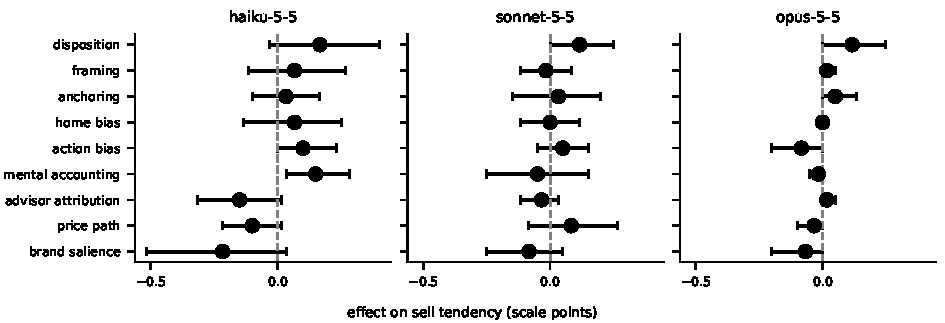
\includegraphics[width=\textwidth]{../figures/fig1_forest_acl.pdf}
  \caption{Matched pair effects on the categorical measure at \texttt{high}
  effort, with 95\% bootstrap intervals over matched pairs. Zero means the
  irrelevant cue changed nothing. Panels share an $x$ axis and run weakest to
  strongest model; Figure~\ref{fig:forestpct} in Appendix~\ref{app:pctmeasure}
  is the same plot on the continuous measure.}
  \label{fig:forest}
\end{figure*}
\else
\begin{figure}[tb]
  \centering
  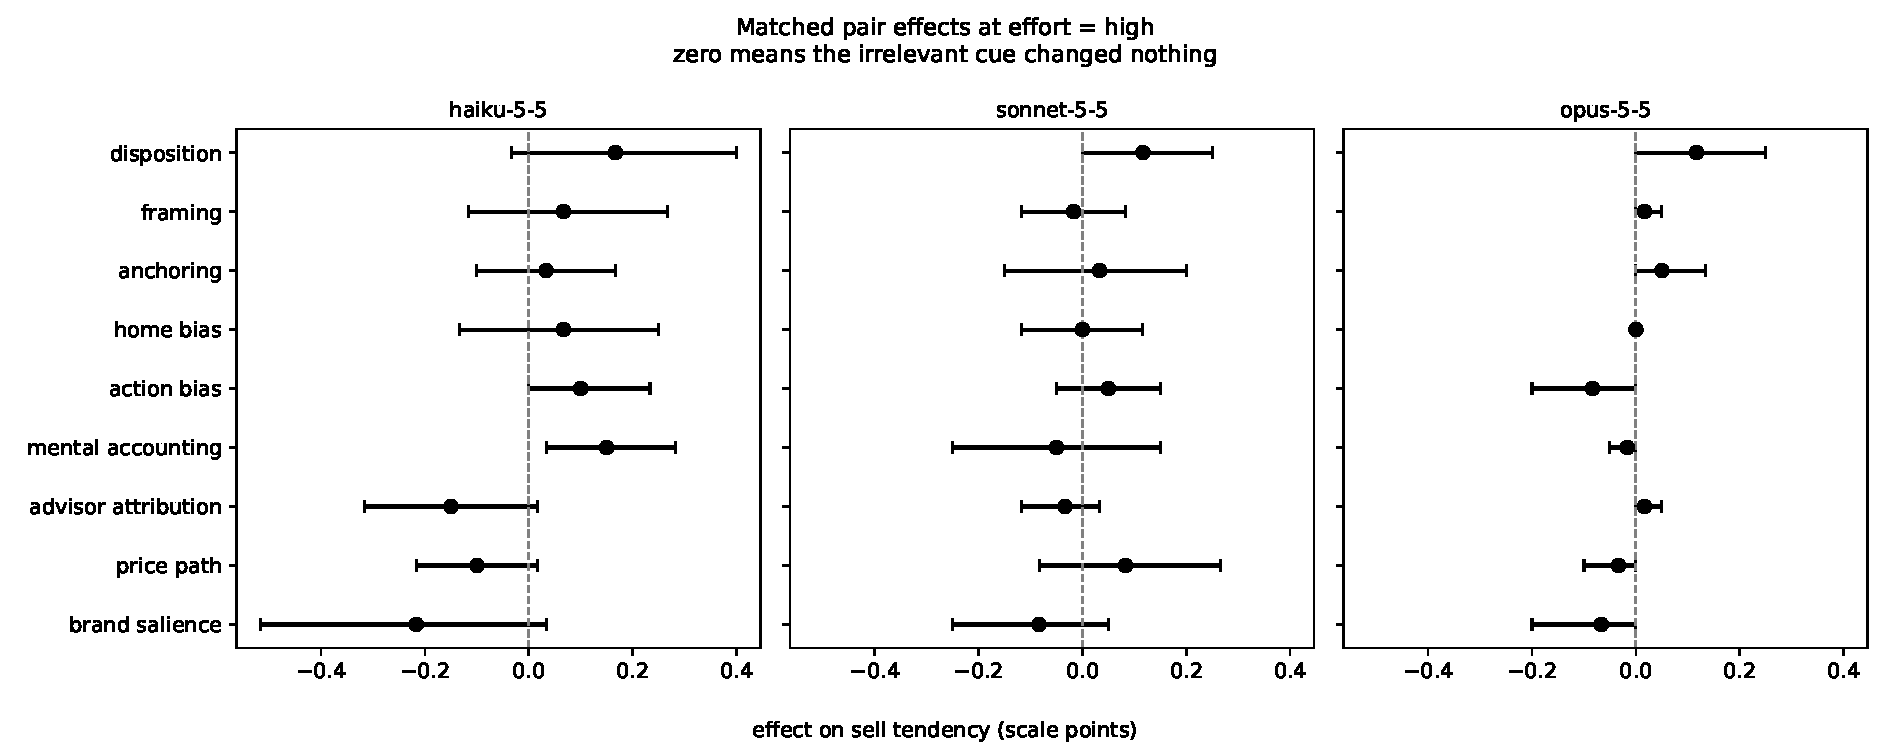
\includegraphics[width=\linewidth]{../figures/fig1_forest.pdf}
  \caption{Matched pair effects with 95\% bootstrap intervals. Zero means the
  irrelevant cue changed nothing.}
  \label{fig:forest}
\end{figure}
\fi

\ifsubmission
The figure the abstract quotes pools over model and effort, which the design
varies, and it hides a split: clear of zero in Haiku and Sonnet on both
measures, and in Opus indistinguishable from zero, its sign changing as
effort rises (\movedref{app:disposition}).
\else
\movedhead{The pooled disposition figure, by model}
\label{sec:disposition}\label{app:disposition}
The abstract states the disposition reversal once, over the whole study,
because the direction is a claim about these models rather than about one
cell of a design that varies model and effort. That pooling is a secondary
aggregation and not a registered quantity, and it is not uniform across the
three models. The figures below come from \texttt{analysis/aggregate.py},
which imports the bootstrap, the seed and the matched pair definition from
the registered script and changes only the grouping.

\begin{table}[t]
  \centering
  \footnotesize
  \begin{tabular}{lrl}
    \toprule
                     & Effect & 95\% CI \\
    \midrule
    \multicolumn{3}{l}{\textit{Categorical, sell tendency}} \\
    Haiku            & $+0.367$  & $[+0.211, +0.533]$ \\
    Sonnet           & $+0.328$  & $[+0.172, +0.494]$ \\
    Opus             & $+0.022$  & $[-0.106, +0.144]$ \\
    All three pooled & $+0.239$  & $[+0.148, +0.331]$ \\
    \midrule
    \multicolumn{3}{l}{\textit{Continuous, percentage points}} \\
    Haiku            & $+21.194$ & $[+12.722, +30.389]$ \\
    Sonnet           & $+15.556$ & $[+8.111, +23.667]$ \\
    Opus             & $+3.378$  & $[-2.567, +9.350]$ \\
    All three pooled & $+13.376$ & $[+8.826, +18.037]$ \\
    \bottomrule
  \end{tabular}
  \caption{The disposition family pooled over effort, by model, and over
  both factors. Positive is the reversal: more willing to sell the position
  held below its cost basis. Each model rests on 36 matched pairs and the
  pooled row on 108. Produced by \texttt{analysis/aggregate.py}, which
  verifies itself against the registered per-cell figures before reporting.}
  \label{tab:disposition}
\end{table}

Two of the three models carry the reversal with an interval clear of zero on
both measures. Opus does not, and the reason is not that Opus is unbiased on
this family. Its effect changes sign as effort rises: on the continuous
measure it runs $-6.417$ at \texttt{low}, $+9.133$ at \texttt{medium} and
$+7.417$ at \texttt{high}, and on the categorical measure $-0.183$, $+0.133$
and $+0.117$. Pooling over effort averages one negative cell against two
positive ones and returns almost nothing. The absolute effect still falls
monotonically, which is what H10 asserts, so these cells are among the nine
qualifying falls; the fall simply passes through zero instead of stopping
short of it. At \texttt{low} effort Opus is the one cell in the study that
points the human way on this family, and it is also the only model whose
disposition sign the manipulation moves.

The practical reading is that the reversal is a property of these two
models at every effort level and of the third at two of three, and that a
single pooled number is the wrong instrument for a quantity the design was
built to split. It is reported because the abstract quotes it, and a figure
in an abstract should be traceable to the grouping that produced it. The
registered unit of analysis is the cell, in Figure~\ref{fig:forest} and the
per-cell tables.

\fi

\ifsubmission
The sign is also reversed against the human field estimates. Investors in
brokerage data realise their winners about half again as often as their
losers \citep{odean1998losses}; these models do the opposite. A field study
of accounts and a prompt battery are different instruments, so the comparison
is indicative; Appendix~\ref{app:humanbaselines} sets out each family's human
anchor and what it can support.
\else
\movedhead{Comparison to human baselines}
\label{sec:humanbaselines}\label{app:humanbaselines}
Two prior measurements of the disposition effect in language models should be
read before the comparison below, because neither reproduces the human
direction. \citet{malberg2025comprehensive}, testing thirty biases across
twenty models, report the disposition effect as one of only two with a strong
negative average, meaning their models preferred change to the status quo.
\citet{yee2026calibrating}, across four models and 24{,}000
agent-scenario pairs, report disposition effects near zero relative to human
benchmarks. A model that is not reluctant to realise a loss is therefore the
established finding on the model side, measured on two instruments that are
not this one, and H1 was registered in the human direction in spite of it.

The human benchmark for the disposition family is
\citet{odean1998losses}, who scores 10,000 accounts at a nationwide discount
brokerage from 1987 to 1993 by the proportion of gains realised against the
proportion of losses realised. Aggregated over the whole period his Table~I
reports PGR of 0.148 against PLR of 0.098, a difference of 0.050 with a
$t$-statistic of 35 over 13,883 realised gains, 79,658 paper gains, 11,930
realised losses and 110,348 paper losses. Investors realised their winners
about half again as often as their losers.

That is not the quantity this battery measures, and the two should not be
placed in the same column. Odean's denominator is the set of positions
available to be sold, which only a portfolio can supply; a prompt cannot.
What transfers between the two instruments is the sign. A human investor is
more willing to sell a position held at a gain than one held at a loss, so
the disposition family here predicts a lower sell tendency in the loss arm
than in the gain arm, which is the negative direction registered for H1 in
Table~\ref{tab:hypotheses}. Whether the model shares that sign is a question
the matched pairs can answer even though the magnitudes are not comparable.

The models do not share that sign. H1 predicted a negative effect, a lower
sell tendency in the loss arm, and the measured effect is positive in eight
of the nine model by effort cells on both measures. The exception is Opus at
\texttt{low} effort, discussed below. Aggregating the disposition family over
all nine cells, which the analysis plan does not register as a quantity and
which is reported here as a secondary aggregation rather than a confirmatory
test, the effect is $+0.239$ $[+0.148, +0.331]$ on the categorical measure
over 108 pairs, 47 of them positive against 11 negative, and $+13.376$
$[+8.844, +18.104]$ on the continuous measure, 64 positive against 16
negative. Per model, the aggregate is $+0.367$ $[+0.206, +0.533]$ in Haiku,
$+0.328$ $[+0.178, +0.500]$ in Sonnet, and $+0.022$ $[-0.106, +0.144]$ in
Opus.

Read against Odean's sign, this is a reversal rather than an absence. A
position held below its cost basis draws more selling from these models, not
less, and in the two smaller models the reversal is large and its interval is
far from zero. H1 is recorded as a failed directional prediction. The
pre-registered sign in \texttt{analysis/directions.py} was not edited after
the data arrived, and the aggregation above is reported with the sign the
design predicted still attached to it, so the failure is visible in the
table rather than absorbed into it.

Two independent instruments already pointed this way.
\citet{malberg2025comprehensive} score the disposition effect as one of only
two biases out of thirty with a strong negative average, which on their
coding means a preference for change, and \citet{yee2026calibrating} find
disposition effects near zero against human benchmarks. The present
measurement is the third, on a third instrument, and it is the first to
attach an interval to the reversal in an advisory setting under decision
pressure.

\fi

\subsection{Reasoning effort}
H10 is registered conditionally: for any family with a non-zero effect at
\texttt{low}, the absolute effect at \texttt{high} will be smaller. The
pre-registration keeps the two exploratory families out of every pooled
confirmatory statement, so the registered reading uses the seven confirmatory
families. Four qualify on the categorical measure and five on the continuous,
and in all nine the absolute effect at \texttt{high} is smaller. \ifsubmission
The largest fall is Haiku's disposition family, from $+44.167$ to $+8.500$
percentage points of the position, and the smallest Opus on anchoring, from
$+7.833$ to $+5.583$; Appendix~\ref{app:h10cases} lists all nine with both
endpoints and Figure~\ref{fig:effort} in Appendix~\ref{app:trajectories}
plots every family's trajectory.
\else
On the
categorical measure they are Haiku and Sonnet on disposition, falling from
$+0.750$ to $+0.167$ and from $+0.383$ to $+0.117$, and Opus on framing and
anchoring, from $+0.300$ to $+0.017$ and from $+0.233$ to $+0.050$. On the
continuous measure they are Haiku on disposition and home bias, from
$+44.167$ to $+8.500$ and from $+11.617$ to $+4.000$, Sonnet on disposition,
from $+18.500$ to $+4.167$, and Opus on framing and anchoring, from $+15.167$
to $+1.750$ and from $+7.833$ to $+5.583$.
\fi

Adding the two exploratory families makes the count ten of eleven. Opus on
brand salience shrinks, from $-0.233$ to $-0.067$; Haiku on price path does
not, moving from $-0.083$ to $-0.100$, so its absolute effect grows by 0.017
on a three-point scale. That is the only qualifying case anywhere that moves
against H10. Its magnitude is inside the instrument's resolution, one scale
point divided by the trial count, but a count of ten of ten that reaches ten
by dropping the case that fails is not worth reporting.

The probability of this pattern under the null is \textit{not} $2^{-9}$.
H10 selects families on having a non-zero effect at \texttt{low} and then
asks whether a second measurement of the same quantity is smaller, and
selection on a noisy baseline shrinks on re-measurement even when nothing
changed, because the cells clearing the filter are disproportionately those
whose noise pointed away from zero \citep{barnett2005regression}.
\ifsubmission\else
\movedref{sec:h10null} measures the real null by running the registered
rule on data whose effort labels have been shuffled.
\fi

H10-null is therefore not supported on its own terms: the parameter raised
generation and the recommendation changed with it, so the effect is not
confined to the justification.

The reduction is not uniform across families, and the shape of the exception
matters. Table~\ref{tab:effort} gives the pooled picture. The slope of
absolute effect per effort step excludes zero only in Opus, on both measures,
and contrasts of slopes exclude zero for Haiku against Opus, $+0.067$
$[+0.016, +0.119]$, and Sonnet against Opus, $+0.085$ $[+0.033, +0.136]$, on
the categorical measure only.

A pooled slope near zero in Haiku alongside a 36-point collapse on its
disposition family can only happen if other families moved the other way,
and they did. Spread and mean both fall in all six rows of
Table~\ref{tab:effort}, but the fall in spread excludes zero in four of them
and the per-step slope on the mean in two, both of them Opus, so the two are
separable here. Haiku is the clear case of compression without reduction:
its three largest families fall, disposition by $35.67$ points of the
position, while five of the remaining six rise, so the standard deviation of
the nine drops from $12.91$ to $2.91$ and the pooled slope stays
indistinguishable from
zero.
\movedref{sec:rtm} shows the count of six is weaker evidence than it
appears and the magnitudes stronger.

\begin{table*}[t]
  \centering
  \small
  % Default tabcolsep puts this 5.6pt over the measure in the single column
  % reading build, where a table* is set to the full text width.
  \setlength{\tabcolsep}{4pt}
  \begin{tabular}{@{}llcccc@{}}
    \toprule
    Model & Meas. & mean low $\rightarrow$ high & slope per step [95\% CI]
          & sd low $\rightarrow$ high & $\Delta$sd [95\% CI] \\
    \midrule
    Haiku & cat & $0.17 \rightarrow 0.12$ & $-0.025$ $[-0.063, +0.014]$
          & $0.22 \rightarrow 0.05$ & $-0.160$ $[-0.231, -0.033]$ \\
    Sonnet & cat & $0.12 \rightarrow 0.05$ & $-0.006$ $[-0.046, +0.030]$
          & $0.10 \rightarrow 0.03$ & $-0.070$ $[-0.157, +0.000]$ \\
    Opus & cat & $0.16 \rightarrow 0.04$ & $-0.092$ $[-0.127, -0.056]$
          & $0.08 \rightarrow 0.04$ & $-0.047$ $[-0.133, -0.008]$ \\
    Haiku & pct & $9.12 \rightarrow 5.42$ & $-1.831$ $[-3.907, +0.143]$
          & $12.91 \rightarrow 2.91$ & $-10.002$ $[-14.210, -3.314]$ \\
    Sonnet & pct & $5.99 \rightarrow 2.32$ & $-0.787$ $[-2.657, +0.880]$
          & $5.06 \rightarrow 1.56$ & $-3.499$ $[-7.800, -0.293]$ \\
    Opus & pct & $6.14 \rightarrow 3.52$ & $-2.758$ $[-4.156, -1.371]$
          & $3.82 \rightarrow 2.41$ & $-1.420$ $[-5.048, +0.575]$ \\
    \bottomrule
  \end{tabular}
  \caption{Reasoning effort pooled over the nine families. \texttt{cat} is
  the four-point sell tendency, \texttt{pct} the percentage of the position;
  mean and sd are over the nine absolute family effects, intervals are
  percentile bootstrap over pairs. Sonnet's \texttt{medium} cell duplicates
  its \texttt{low} cell (\movedref{app:sonnetmedium}), flattening its
  per-step slope.}
  \label{tab:effort}
\end{table*}

\ifsubmission\else
\begin{figure}[tb]
  \centering
  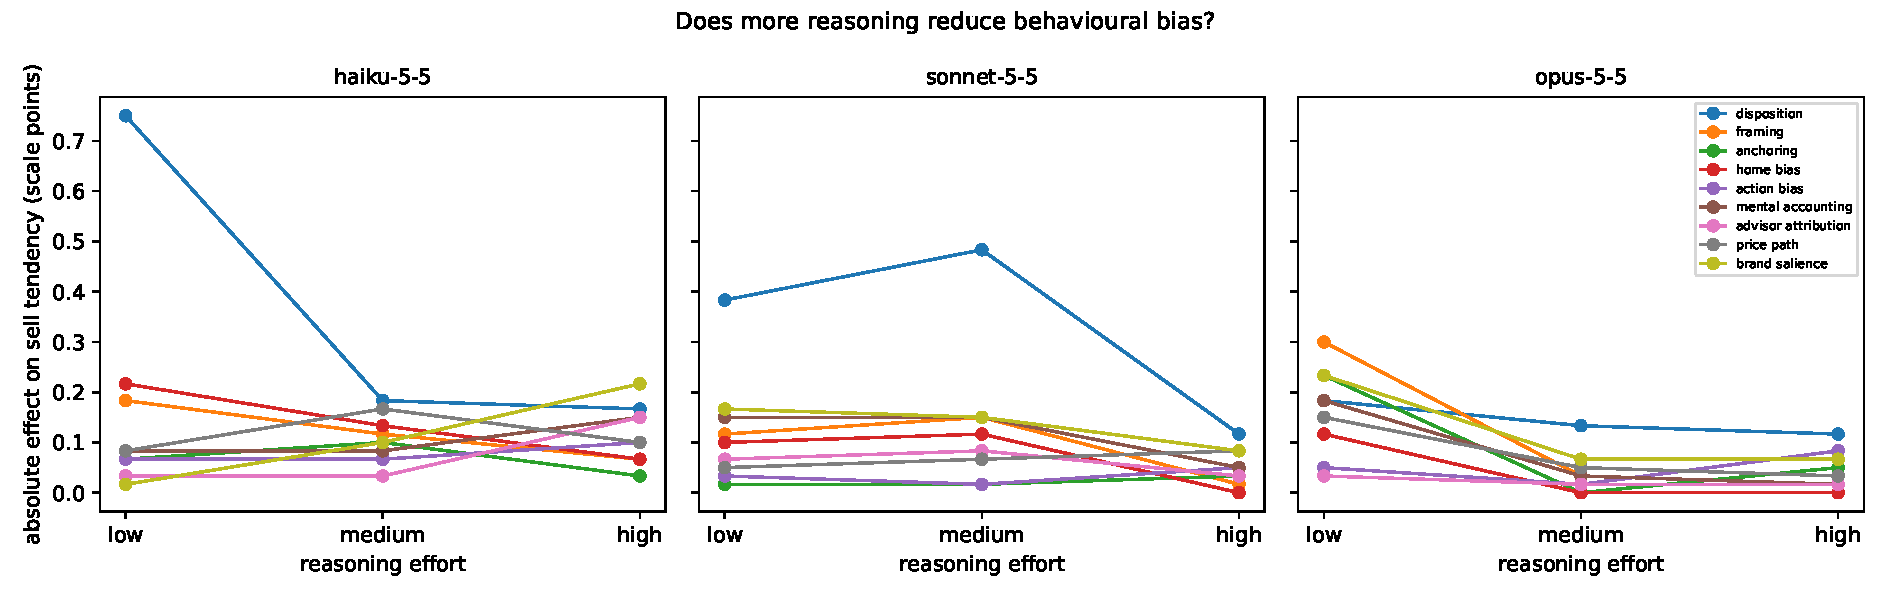
\includegraphics[width=\linewidth]{../figures/fig2_effort.pdf}
  \caption{Absolute effect against reasoning effort.}
  \label{fig:effort}
\end{figure}
\fi

\ifsubmission
A qualifying case therefore shrinks on re-measurement at a rate above one
half even when effort does nothing. Shuffling the effort labels within model
and item over 400 replicates and running the registered rule on each puts
that rate at 0.654 on the confirmatory families and 0.706 across all nine,
and the probability that every qualifying case shrinks at 0.0125 and 0.0200,
a factor of six on the coin-flip null.
Appendix~\ref{app:h10null} gives the two features that cut the other way.
\else
\movedhead{What the null for H10 actually is}
\label{sec:h10null}\label{app:h10null}
H10 is a conditional hypothesis, and the condition does work that a naive
count ignores. The rule selects a family on having a non-zero effect at
\texttt{low} and then asks whether a second, independent measurement of the
same quantity is smaller. A family qualifies partly because its true effect
is large and partly because its noise at \texttt{low} happened to point away
from zero, and the second measurement does not inherit that luck. So the
qualifying cases shrink on re-measurement at a rate above one half even when
effort does nothing at all, which is the standard regression artefact of
selecting on a noisy baseline \citep{barnett2005regression}. Reporting
$2^{-n}$ against a count of $n$ successes treats the rate as one half and
overstates the evidence.

The rate can be measured rather than assumed. In
\texttt{analysis/h10\us placebo.py} the effort label is shuffled among the
responses to the same item within a model, over 400 shuffles, and the
registered H10 rule including its bootstrap filter is run on each shuffled
replicate. The rule, the sample sizes and the item set are untouched; only
the labels move, so no real effect of effort can survive and whatever the
rule still finds is the artefact alone. Using the seven confirmatory
families, a qualifying case shrinks with probability 0.654, not 0.500, and
the running estimate is stable from the first hundred shuffles. Across all
nine families the rate is 0.706. The rate is further from one half in the
inclusive set because the two exploratory families have the smallest true
effects, so a larger share of what qualifies them is noise.

The matched null event is the one H10 asserts: every qualifying case shrinks.
Its measured probability is 0.0125 on the confirmatory families and 0.0200
across all nine. Against the coin flip's $2^{-9}$ for the nine confirmatory
cases observed, one in five hundred and twelve, the measured figure is larger
by a factor of six. The observed result is therefore unlikely under the null,
but by well under an order of magnitude less than a count alone suggests, and
the paper claims the measured figure.

Two features of the measurement are worth stating because they cut in
opposite directions. The shuffled replicates qualify more cases than the real
data does, 11.48 on average with a range of 6 to 20 against the observed 9,
so the joint event is being evaluated over a longer run of cases than the one
actually reported; that makes 0.0125 smaller than the figure a nine-case
comparison would give. Raising the measured per-case rate to the ninth power
gives 0.022, which is the matched figure if qualifying cases were
independent. They are not, since cases within a model share the same
responses, so the truth is above the directly measured 0.0125 and the paper
uses that bound rather than the smaller number. Either way the conclusion is
the same: the pattern is unlikely under the null by roughly one part in fifty
to one part in eighty, and not one part in five hundred.

\fi

\ifsubmission
A falling spread has an innocent explanation that would account for the whole
result: sampling error inflates a spread, and inflates an absolute value most
near zero, so if the error were larger at \texttt{low} than at \texttt{high}
the spread would fall with no change in the model's bias.
Appendix~\ref{app:rtm} tests that three ways within wave 1. Subtracting the
trial level sampling variance, the part unambiguously measurement error,
leaves the fall intact in all six combinations, and no shuffle of the effort
labels in 2{,}000 reproduces Haiku's compression on either measure,
$p < 0.0005$. Under a harsher floor that charges item to item variation to
error the fall survives in three of six. We therefore state the mechanism as
a finding about the weakest model and a conjecture about the strongest. None
of those tests can estimate the error from anything but the pairs carrying
the effect; the remedy they point to is more items per family.
\else
\movedhead{Is the compression regression to the mean?}
\label{sec:rtm}\label{app:rtm}
A falling spread has an innocent explanation that would account for the whole
result. Each family effect is estimated from twelve pairs with five trials an
arm, so each carries sampling error; sampling error inflates the spread of
the estimates above the spread of the truth, and it inflates an absolute
value most where the true effect is near zero. If that error were larger at
\texttt{low} effort than at \texttt{high}, the spread would fall with effort
even if nothing about the model's bias had changed. The analysis in
\texttt{analysis/robustness.py} tests this three ways. None of it is
pre-registered.

\paragraph{Removing the measurement error.} The variance of the nine
estimates is the variance of the truth plus the mean sampling variance of an
estimate, so the second can be subtracted. Two floors bracket the answer.
The narrow floor counts only the trial resampling variance of each pair's own
difference, which is unambiguously measurement error; subtracting it leaves
the spread almost unchanged and the fall survives in all six combinations,
for instance Haiku's continuous spread at \texttt{low} moving from 12.91 to
12.54 and its categorical spread from 0.215 to 0.206. The wide floor instead
counts the whole standard error of the family mean across its twelve pairs,
which also removes the genuine item to item variation within a family; it is
too harsh, because a cue whose effect differs across items is a fact about
the model rather than a measurement fault. Under that floor the fall survives
in three of six: Haiku on both measures and Sonnet on the continuous measure.
The other three cells have no between-family spread left to compress at any
effort level, which is itself worth stating plainly. In Opus and in Sonnet on
the categorical measure the nine families are indistinguishable from one
another once item variation is charged against the estimate, so for those
cells the design can establish that the raw spread falls but not that a real
between-family spread existed to begin with.

\paragraph{The noise runs against the finding in two models.} The trial-level
noise floor is not constant across effort, and its direction matters. In
Haiku it rises from 0.062 to 0.073 on the categorical measure and from 3.10
to 3.53 on the continuous one, and in Sonnet from 0.023 to 0.056, so in those
models the \texttt{high} effort estimate is the noisier one. Noise inflates a
spread, so this biases the comparison against the result, and the spread
falls anyway. In Opus the floor falls with effort, from 0.039 to 0.024 and
from 1.49 to 1.16, which is the direction that would help the result; Opus is
therefore the model whose compression rests most on the correction, and it is
also the one where the wide floor leaves nothing.

\paragraph{A placebo.} Shuffling the effort label among the responses to the
same item within a model destroys any real effect of effort and leaves
everything else intact. Over 2{,}000 shuffles the spread falls in all six
combinations 6.25\% of the time, so the \textit{count} of six out of six is
not on its own strong evidence and should not be reported as though it were.
The magnitudes are a different matter. Every one of the six observed changes
is more negative than almost every shuffle: $p < 0.0005$ for Haiku on both
measures, where no shuffle in 2{,}000 reached the observed change, $p =
0.0065$ and $p = 0.0010$ for Sonnet, and $p = 0.0080$ and $p = 0.0100$ for
Opus. The reason the count is weak while each magnitude is strong is that the
six cells are positively correlated under the placebo, so a shuffle that
makes one fall tends to make several fall.

\paragraph{Leaving a family out.} Dropping each family in turn and recounting
leaves six of six intact in eight of the nine cases and five of six when
framing is dropped, so the result is not carried by any single cue.

Taken together: the compression is real in Haiku, where it is large and
survives every correction; real in Sonnet on the continuous measure; and in
Opus and Sonnet's categorical measure it is a fall in a spread that was never
established to exceed measurement error. The claim in the title of this
section is answered no for Haiku and not fully excluded for Opus. The paper
states the mechanism as a finding about the weakest model and a conjecture
about the others, and the remedy is more items per family rather than more
trials per item, since the limiting quantity is the twelve pairs.

\fi

\ifsubmission
That remedy was taken. A replication wave of
9{,}720 responses, twelve further pairs per family on Haiku and Sonnet,
reproduces the pattern, per cell effects correlating $+0.467$ and $+0.484$
over 54 cells at $p$ below 0.001. The magnitudes attenuate, and the cause is
measurable out of sample: none of the shrinkage is design wide, and all of it
sits in the largest cells, where the top quartile loses half its magnitude
and the other three do not move (Appendix~\ref{app:replication}).
\else
\movedhead{Does any of this replicate?}
\label{sec:replication}\label{app:replication}
Every effect above comes from one draw of twelve matched pairs per family. A
second draw was collected to separate what is a property of these models from
what was a property of that draw. It was decided on after wave 1 had been
read, which is the kind of deviation that most needs declaring, and the
registration declares it along with the three readings it commits to in
advance: wave 1 alone, wave 2 alone, and the two pooled. Wave 1 is reported
unchanged everywhere else in this paper, and none of this section is
pre-registered.

\paragraph{What the second wave is.} Twelve further pairs per family, at the
same nine families and three effort levels, built by the same generator with
per family seeds derived from the wave number, so the new items are a fresh
draw from the same distribution rather than a hand picked set. The analysis
is the registered one: the same matched pair definition, the same bootstrap
seed, the same Holm correction within a cell. Running it on wave 1 alone
reproduces the committed output byte for byte, which is the regression test
that adding a wave did not quietly alter the first one.

\paragraph{What it covers, and what it does not.} Haiku and Sonnet, at all
three efforts and all nine families. Not Opus. The three Opus batches
exhausted the study's API credit part way through and returned an error for
roughly four hundred of their 1{,}080 requests each, which left 37 of 108
pairs per effort holding both conditions, spread unevenly across the families
from seven pairs in one down to two in another. A cell resting on two pairs
is not an estimate, and a reading in which Opus rests on a much smaller item
set than the other two models is not a comparison between models. The rule,
fixed before any Opus wave 2 effect was computed and keyed on coverage alone,
excludes a cell short of its twelve pairs whole rather than analysing what
survived. The partial responses stay in the released data, because deleting
them would make the exclusion unverifiable. Two consequences follow and are
load bearing for everything below: the replication covers two models, and the
pooled reading gives those two twenty four pairs per cell while leaving Opus
at wave 1's twelve, so every gain in power below is theirs alone.

\paragraph{The pattern replicates.} Across the 54 cells both waves carry, the
per cell effects correlate $+0.467$ on the categorical measure and $+0.484$
on the continuous one, with permutation $p$ of 0.0009 and 0.0005. Wave 2's
interval contains wave 1's point estimate for 41 of those cells on the
categorical measure and 43 on the continuous one. Two of 54 cells differ
between the waves by more than their pairs explain, which is 3.7 per cent
against the 5 per cent a true replication produces by construction. Of the
cells significant in wave 1, six of seven keep their sign on the categorical
measure and eight of nine on the continuous one.

\paragraph{Significance does not replicate, and could not have.} Four of 54
cells clear zero on each measure in wave 2 alone and none survives Holm
correction. This restates the power problem that motivated the second wave
rather than contradicting the first: wave 2 is the same size as wave 1 and
has the same permutation floor at twelve pairs, so a sign is what a draw this
size can replicate and a corrected $p$ is not. The pooled reading, where the
pairs actually add, reaches two Holm cleared cells on the categorical measure
and three on the continuous one.

\ifsubmission
\begin{figure*}[t]
  \centering
  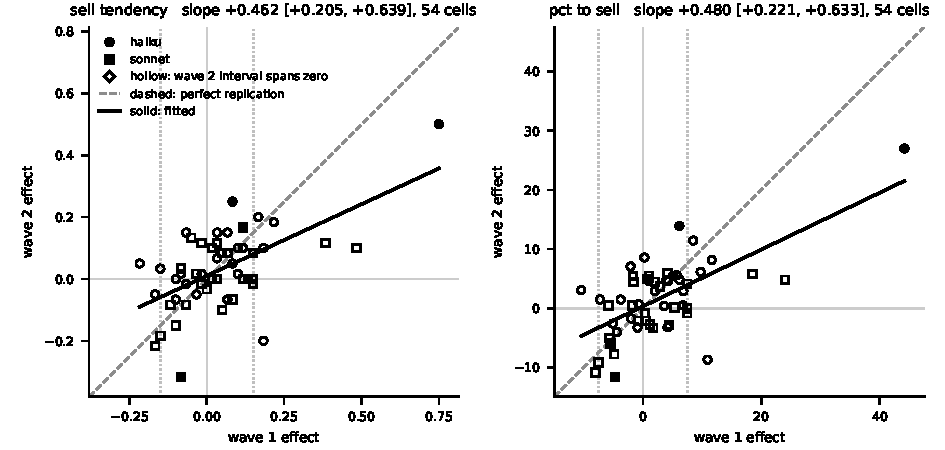
\includegraphics[width=\textwidth]{../figures/fig7_replication_acl.pdf}
  \caption{The 54 cells both waves carry, each plotted at its wave 1 effect
  against its wave 2 effect, on items the first wave never saw. If a
  wave 1 estimate were the truth, the cloud would sit on the dashed identity
  line; if the finding were noise, the cloud would be round. It is neither.
  It tilts, which is the replication, and it tilts at about half the identity
  slope, which is the shrinkage. Both axes carry the same range so that the
  identity line is drawn at forty five degrees and a reader can judge the gap
  by eye. The dotted verticals cut off the top quartile by wave 1 magnitude,
  the band that loses half of itself while the rest of the design does not
  move. A hollow marker is a cell whose wave 2 interval spans zero, which is
  most of them: this is a figure about where the points sit, not about which
  of them are significant.}
  \label{fig:replication}
\end{figure*}
\else
\begin{figure}[t]
  \centering
  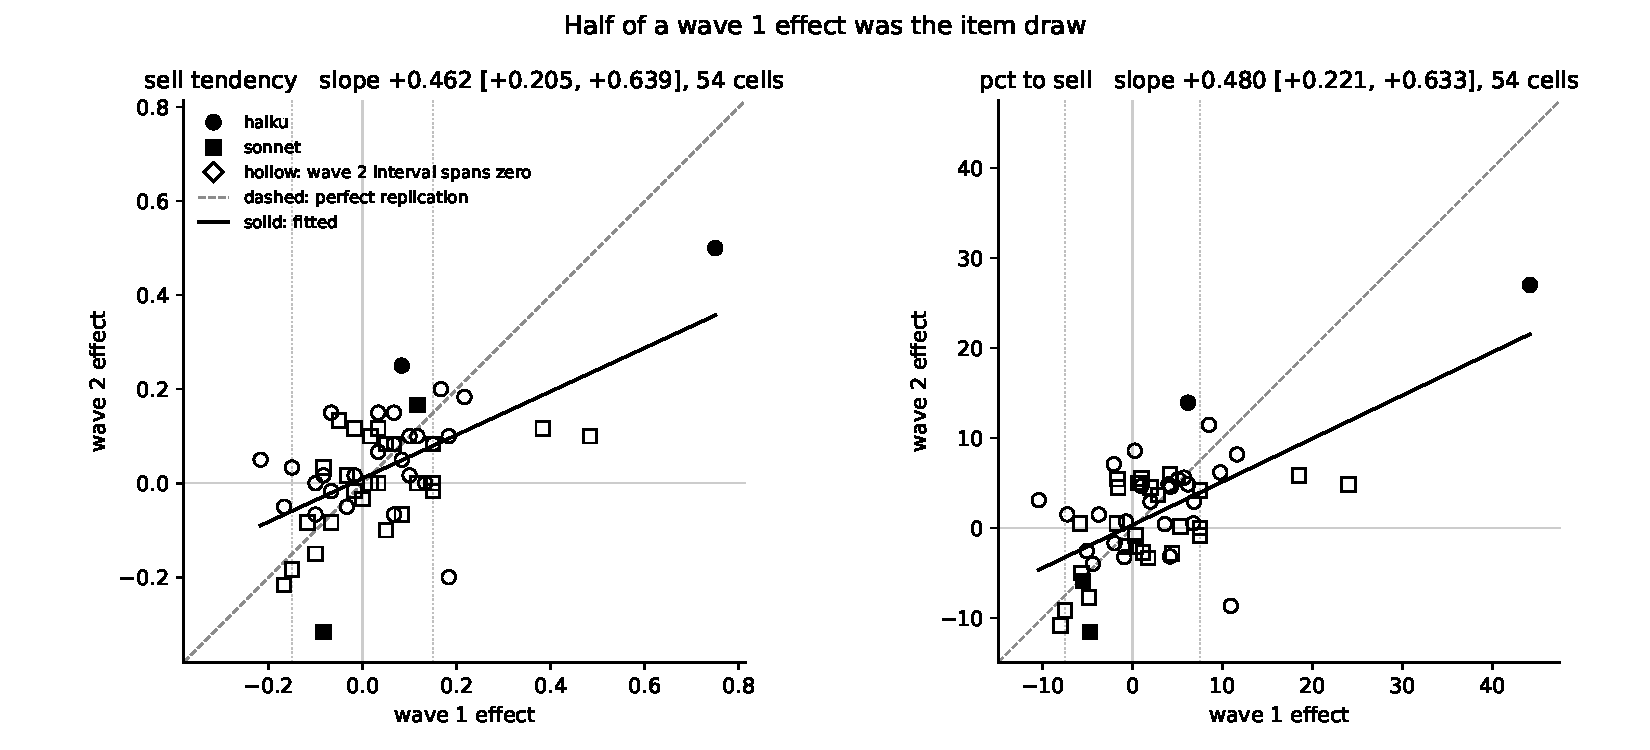
\includegraphics[width=\linewidth]{../figures/fig7_replication.pdf}
  \caption{Wave 2 against wave 1, one point per cell. The dashed line is
  perfect replication and the solid line is the fit. The gap between them is
  the regression to the mean, and the dotted verticals mark the top quartile
  by wave 1 magnitude, where all of it sits.}
  \label{fig:replication}
\end{figure}
\fi

\paragraph{The magnitudes do not replicate, and the reason is measurable.}
The disposition aggregate over the cells wave 2 covers is $+0.347$ $[+0.233,
+0.464]$ in wave 1 and $+0.147$ $[+0.014, +0.281]$ in wave 2; on the
continuous measure, $+18.375$ $[+12.542, +24.361]$ against $+7.728$
$[+0.881, +14.694]$. The between wave differences are $-0.200$ $[-0.375,
-0.022]$ and $-10.647$ $[-19.678, -1.611]$, intervals that exclude zero. Two
fifths of the wave 1 figure comes back. The obvious reading is that something
about the second wave is different, and it is the wrong one. Across all 54
cells, 28 came in smaller on the categorical measure and 26 on the
continuous one, against 27 under no attenuation whatsoever: there is no
general shrinkage to find. The shrinkage is conditional on size. The
correlation between a cell's wave 1 magnitude and the change in its magnitude
is $-0.580$ and $-0.622$, permutation $p$ 0.0001 on both measures. The top
quartile by wave 1 magnitude shrank in ten of thirteen cells, by $-0.117$ and
$-5.821$ on average, while the other three quartiles moved $+0.009$ and
$+0.631$, which is nothing.

\paragraph{One number for all of it.} Regressing each cell's wave 2 effect on
its wave 1 effect gives a slope of $+0.462$ $[+0.205, +0.639]$ on the
categorical measure and $+0.480$ $[+0.221, +0.633]$ on the continuous one,
resampled over cells rather than pairs. A slope of one is what wave 1
estimates being the truth would produce, and both intervals exclude it; a
slope of zero is what noise alone would produce, and both exclude that too.
The slope is therefore the fraction of a wave 1 effect that was signal rather
than a favourable item draw, measured on items the first wave never saw, and
it is a little under a half. Figure~\ref{fig:replication} is that fit, and
it is this section's argument in one picture: a cloud that tilts, at half the
slope it would tilt at if twelve pairs told the truth.

\paragraph{What that is.} Regression to the mean, measured from outside
rather than bounded from inside. A large effect at twelve pairs is partly a
large true effect and partly a favourable item draw, and only the first half
returns on items the first draw never saw. \movedref{sec:rtm} asks whether
the compression result is regression to the mean and can only bracket the
answer within one wave, because the sampling error it wants to subtract is
estimated from the same twelve pairs that carry the effect. A second draw
from the same generator is not subject to that circularity, and it puts a
number on the correction: the slope above, and in the quartile where this
paper's headline findings live, roughly half of a wave 1 magnitude is the
draw.

\paragraph{Both headline magnitudes attenuate, and both directions hold.}
The single cell this paper leads with, Haiku at \texttt{low} effort on the
disposition family, moves from $+0.750$ $[+0.483, +1.033]$ to $+0.500$
$[+0.167, +0.850]$ on the categorical measure and from $+44.167$ $[+28.500,
+60.333]$ to $+27.000$ $[+9.500, +46.333]$ on the continuous one, pooling to
$+0.625$ $[+0.400, +0.858]$ and $+35.583$ $[+22.958, +48.500]$, which still
survive Holm. The compression of the family spread behaves the same way:
Haiku's fall from \texttt{low} to \texttt{high} is $-0.085$ against wave 1's
$-0.160$ categorically and $-4.008$ against $-10.002$ continuously, and
Sonnet's continuous spread falls by $-0.039$ against $-3.499$ while its
categorical spread rises by $+0.020$ against a fall of $-0.070$. The spread
still falls in three of the four model by measure combinations wave 2 covers.
A reader who wants this paper's best estimate of either finding should take
the pooled figure and read the wave 1 figure as the upper end.

\paragraph{Two things the second wave cannot settle.} Opus is absent from it,
so the defect recorded in \movedref{app:disposition}, that Opus spans zero on
the disposition measures because its sign changes with effort, stands exactly
where wave 1 left it: the extension that would speak to it is the one the
budget did not reach. And the two measures are not two tests. They are two
readings of the same answer and they move together, so the attenuation is one
finding whose intervals exclude zero narrowly, not a pair of independent
confirmations.

\fi

\subsection{The continuous measure}
\ifsubmission
Amendment 3 added the continuous measure because the categorical scale was at
ceiling in the pilot, and it earned its place: it finds 22 non-zero cells
against the categorical measure's 10, concentrated where the categorical
scale has least room. \texttt{BUY\us MORE} was never returned by any model at
any effort level, and each model concentrates on a single category. Opus is
the extreme case: its categorical answer barely moves, so that measure finds
3, 0 and 0 non-zero cells across the three effort levels while the graded
percentage inside the one category finds 2, 6 and 5. On the registered
measure alone the strongest model would have looked almost bias-free, an
artifact of a scale with no room in it. The two measures agree on
sign and ordering wherever both move and disagree on 86 of 9{,}720 responses,
every one an Opus \texttt{HOLD} carrying a non-zero percentage to sell and 84
of them at \texttt{low} effort; those rows are kept and never reconciled, as
registered. Appendix~\ref{app:pctmeasure} gives the measure in full.
\else
\movedhead{The continuous measure}
\label{sec:pctmeasure}\label{app:pctmeasure}
Amendment 3 added the continuous measure because the categorical scale was at
ceiling in the pilot, and it earned its place. It finds 22 non-zero cells
against the categorical measure's 10, and the gain is concentrated exactly
where the categorical scale has least room. The four-point scale is
effectively three-point in practice, because \texttt{BUY\_MORE} was never
once returned by any model at any effort level, and each model concentrates
on a single category: \texttt{SELL\_PARTIAL} on 80.8\% of Opus responses,
\texttt{HOLD} on 63.2\% of Sonnet's, and a near-even split between those two
in Haiku. Opus is the extreme case. Its categorical answer barely moves
between conditions, so the categorical measure finds 3, 0 and 0 non-zero
cells at \texttt{low}, \texttt{medium} and \texttt{high}, while the graded
percentage inside that one category moves freely and finds 2, 6 and 5. Two of
the four Holm surviving cells exist only on the continuous measure. This is
the clearest vindication of Amendment 3: on the registered measure alone,
the strongest model would have appeared almost bias-free at every effort
level, and that appearance would have been an artifact of a scale with no
room in it.

The two measures agree on sign and ordering wherever both move, and they
disagree on individual responses rarely and systematically. Eighty-six of
9{,}720 responses, 0.88\%, pair a categorical answer with a contradictory
percentage. Every one of the 86 is Opus; 84 of them are at \texttt{low}
effort, a rate of 2.59\% against 0.06\% at \texttt{high}; and every one is a
\texttt{HOLD} accompanied by a non-zero percentage to sell. These rows are
flagged and kept on both measures, never reconciled, as registered. They also
account for the one cell that breaks the disposition sign pattern: Opus at
\texttt{low} effort is the only cell of nine with a negative disposition
effect, and it is the cell in which the model's two answers are least
coherent with each other.

\fi

\ifsubmission\else% Two column in the submission build, so the wide variant would be scaled to
% a 216pt column and set in 2pt type. The _acl variant is drawn at the width
% it is printed at.
\ifsubmission
\begin{figure*}[t]
  \centering
  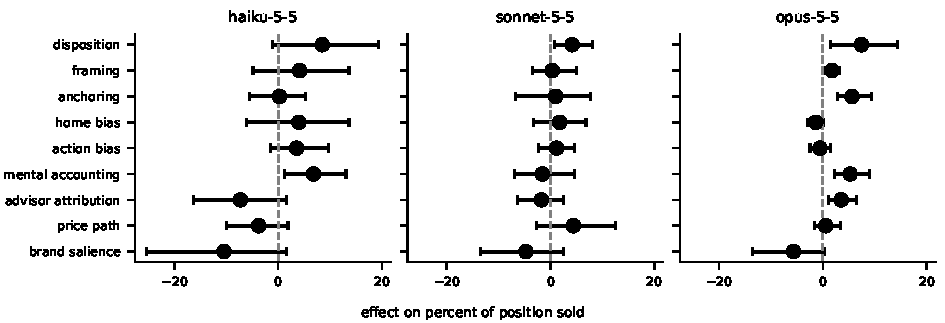
\includegraphics[width=\textwidth]{../figures/fig4_forest_pct_acl.pdf}
  \caption{Matched pair effects on the continuous co-primary measure, the
  percentage of the position the model would sell, at \texttt{high} effort,
  with 95\% bootstrap intervals over matched pairs. The twin of
  Figure~\ref{fig:forest}, which is the same plot on the categorical measure.}
  \label{fig:forestpct}
\end{figure*}
\else
\begin{figure}[t]
  \centering
  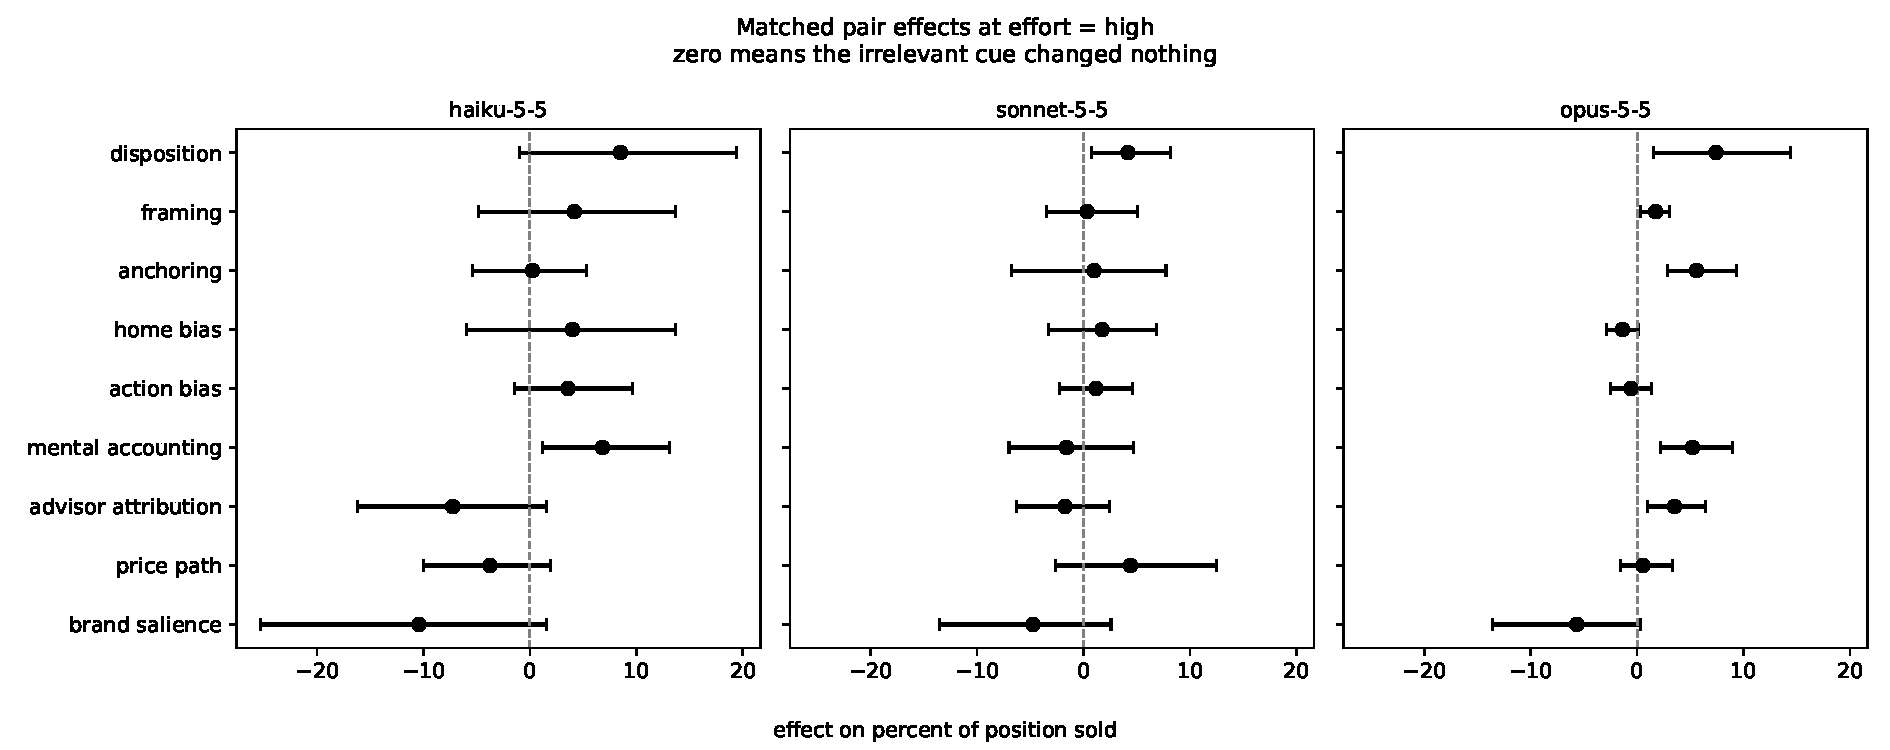
\includegraphics[width=\linewidth]{../figures/fig4_forest_pct.pdf}
  \caption{Matched pair effects on the continuous co-primary measure, the
  percentage of the position the model would sell, with 95\% bootstrap
  intervals.}
  \label{fig:forestpct}
\end{figure}
\fi
\fi

\ifsubmission\else\ifsubmission
\begin{figure*}[t]
  \centering
  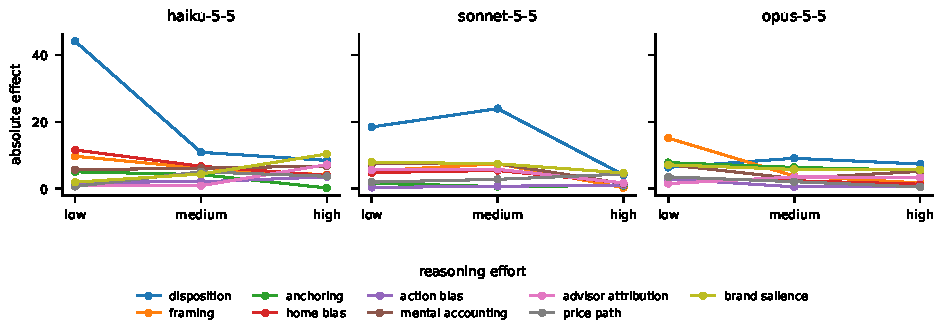
\includegraphics[width=\textwidth]{../figures/fig5_effort_pct_acl.pdf}
  \caption{Absolute family effect on the continuous measure against reasoning
  effort, one line per family, panels weakest to strongest model. The twin of
  Figure~\ref{fig:effort} on the other measure.}
  \label{fig:effortpct}
\end{figure*}
\else
\begin{figure}[t]
  \centering
  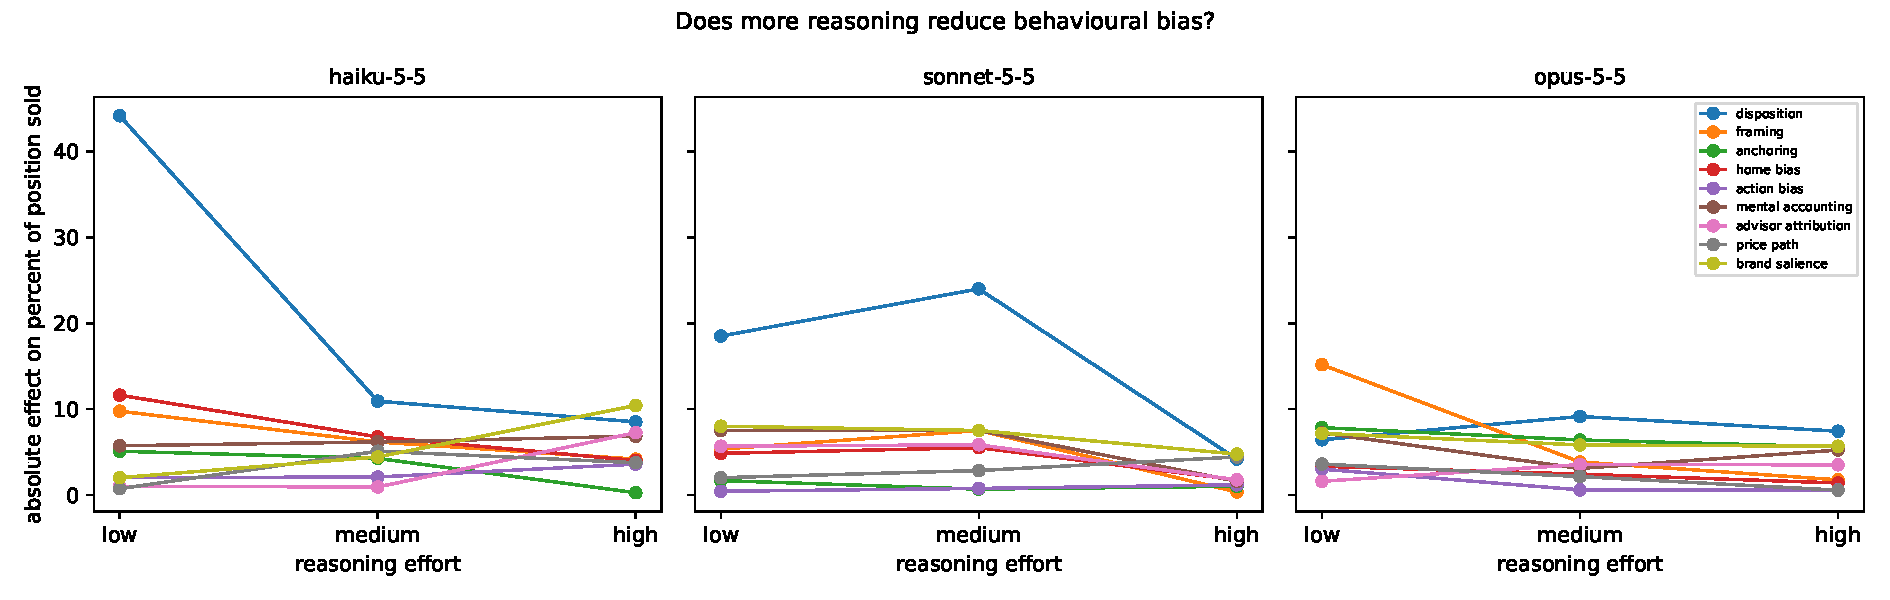
\includegraphics[width=\linewidth]{../figures/fig5_effort_pct.pdf}
  \caption{Absolute effect on the continuous measure against reasoning
  effort.}
  \label{fig:effortpct}
\end{figure}
\fi
\fi

\ifsubmission
The registered concern that effort might buy confidence rather than accuracy
does not materialise: within-item entropy across the five identical repeated
prompts does fall in Opus, from 0.147 to 0.060 bits, but its effect sizes
fall with it (Appendix~\ref{app:variability}).
\else
\movedhead{Response variability}
\label{sec:variability}\label{app:variability}
Because \texttt{temperature} cannot be set on these models, repeated sampling
replaces it and the resulting variability is reported as a result rather than
treated as nuisance. Mean within-item entropy across five identical prompts
separates the models more sharply than effort does: Opus sits between 0.057
and 0.147 bits, Sonnet between 0.053 and 0.311, and Haiku between 0.354 and
0.510. The within-item share of variance in the continuous measure runs from
4.5\% in Sonnet at \texttt{low} effort to 33.6\% in Haiku at \texttt{high}.
Most variance is between items, which is what an instrument that measures its
stimulus should show, but a third of it is within item in Haiku, so a single
sample per item would have been closer to a coin flip than to a measurement.

The pre-registration singles out one combination as the worst outcome for
deployment: an effect size that does not move while entropy falls, which
would mean the model becoming more confident in the same biased answer. It
does not occur. In Haiku and Sonnet entropy rises with effort, from 0.354 to
0.479 and from 0.054 to 0.311, while their absolute effects fall or hold. In
Opus entropy does fall, from 0.147 at \texttt{low} to 0.060 at
\texttt{high}, but its absolute effect falls with it and is the one pooled
slope whose interval excludes zero, so the rising confidence attaches to a
less biased answer rather than to the same one.

\begin{figure}[t]
  \centering
  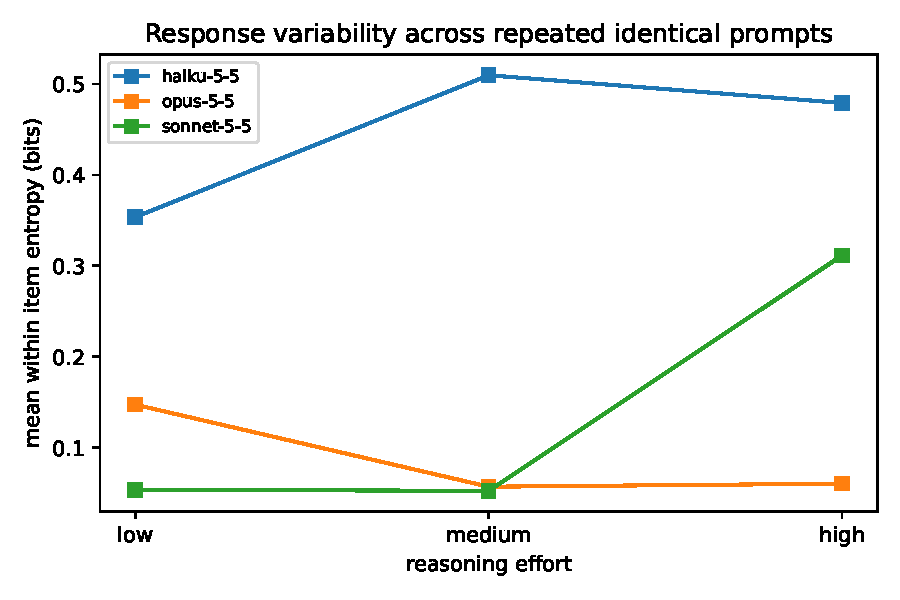
\includegraphics[width=0.7\linewidth]{../figures/fig3_entropy.pdf}
  \caption{Within-item entropy across five identical repeated prompts.}
  \label{fig:entropy}
\end{figure}

\fi

% Printed in both builds, and sec_mediator.tex carries no \movedhead of its
% own as a result. The two labels are referenced from shared prose, so they
% have to resolve to a Section in the reading build as well as the
% submission one, which means the heading they attach to has to exist in
% both.
\subsection{The budget and the behaviour are not the same variable}
\label{sec:lengthorlabel}
\label{sec:mediator}
\ifsubmission
This data can test the identification argument of
Section~\ref{sec:deliberation} rather than assert it, because it holds both
variables: the effort parameter, set before the model sees the item, and
output tokens, chosen by the model. Running the paper's own arithmetic three
ways on the same 9{,}720 responses, changing only which responses enter each
pair mean, gives three answers, and none of this subsection is
pre-registered. Set exogenously, the mean absolute family effect falls in six
of six model by measure combinations. Read observationally across items, bias
is \textit{higher} where the model wrote more, Spearman $+0.190$ categorical
and $+0.154$ continuous over 972 pairs. Read within a single item, where only
the model's sample to sample choice of length differs, nothing survives: four
of nine cells fall, which is chance. Token count is an item property twice
over, so splitting on it re-weights the cues averaged.
Appendix~\ref{app:mediator} gives all three designs.
\else
% No \movedhead here, unlike the other moved sections. body.tex prints this
% heading in both builds, because sec:mediator and sec:lengthorlabel are
% referenced from shared prose and so have to resolve to a Section in both.
% A \movedhead as well set the title twice in the reading build, as an empty
% subsection followed by the real one.
\label{app:mediator}
The argument for setting the reasoning budget through the API rather than
measuring how much reasoning a response contains is made in
Section~\ref{sec:deliberation} on identification grounds: a measure read off
the response is produced by the same forward pass as the answer, so it cannot
separate reasoning that helped from reasoning that a hard item provoked. This
data can test that argument instead of asserting it, because it holds both
variables. The effort parameter is exogenous, set before the model sees the
item. Output tokens are endogenous, chosen by the model for each response.
They are not the self-reported analytical-reasoning indicator used by
\citet{bini2026behavioral}, but they are the same class of variable: a
within-cell, model-chosen measure of how much reasoning a response contains,
with no experimental control over it. None of this subsection is
pre-registered; it was written after the data were in hand.

The parameter does set reasoning volume, so the two variables are not
measuring different constructs. Output tokens rise from \texttt{low} to
\texttt{high} by a factor of 2.33 in Haiku, 2.44 in Opus and 2.91 in Sonnet,
and the distributions barely overlap: 0.1\% of Haiku's and Opus's
\texttt{low} effort responses exceed the median \texttt{high} effort
response, 0.0\% of Sonnet's, and in the other direction 0.0\%, 0.0\% and
3.5\%. If an observational measure of reasoning volume recovers the causal
effect of reasoning volume anywhere, it should do so here.

It does not. \texttt{analysis/mediator.py} runs the paper's own arithmetic
three ways on the same 9{,}720 responses, with the same families, items and
statistics, changing only which responses enter each pair mean.

\paragraph{Exogenous.} Comparing effort levels, the mean absolute family
effect falls from \texttt{low} to \texttt{high} in all three models on both
measures, by $-0.120$, $-0.069$ and $-0.050$ on the categorical measure for
Opus, Sonnet and Haiku, and by $-2.628$, $-3.667$ and $-3.700$ on the
continuous one. Six of six.

\paragraph{Endogenous, between items.} Within a single model and effort cell
the effort label is constant, but generation length still varies widely from
item to item. If deliberation itself is what reduces bias, then holding the
label fixed, pairs on which the model happened to generate more should show
less bias. They show more. The Spearman correlation between a pair's mean
output tokens and its absolute effect, pooled across all nine cells with the
cell means removed from both variables so that only within-cell variation
contributes, is $+0.190$ ($p = 0.0001$) on the categorical measure and
$+0.154$ ($p = 0.0001$) on the continuous measure, over 972 pairs. The
relationship is positive in 17 of the 18 cell by measure combinations and
reaches $p < 0.05$ in eight of them. Taken as a median split instead, so that
the statistic matches the one used for the exogenous comparison, the mean
absolute effect is lower in the heavier half in one cell of nine on both
measures, and pooled over effort and bootstrapped over pairs the contrast is
positive in all three models on both measures, with Haiku on the categorical
measure excluding zero in the wrong direction at $+0.066$ $[+0.014, +0.143]$.
Between cells, bias falls as effort rises. Within cells, bias rises with
length. The two slopes have opposite signs.

\paragraph{Endogenous, within item.} Two readings of that reversal were
available. The first is that the exogenous budget and the model's own
allocation of tokens are distinct interventions with distinct effects. The
second is reverse causation: an item that provokes bias also provokes a
longer answer, so length is an index of item difficulty rather than of
deliberation. A third design separates them. Inside one model by effort cell,
split the five trials of each single item at that item's own median token
count. The stimulus, the family, the company and the effort setting are then
identical across the split, and only the model's sample to sample choice of
how much to write differs. The reversal disappears and nothing takes its
place: the mean absolute effect falls in four of nine cells, which is what
chance gives, and every pooled interval contains zero, the largest being
$-0.585$ $[-2.896, +1.999]$ for Haiku on the continuous measure. The positive
association is therefore a property of the item, not of the response, and the
difficulty reading is the one the data support.

An observational study of these responses would thus have reported that
reasoning makes the bias worse, or that it does nothing, depending on whether
it conditioned on the item. The experiment reports that it reduces the bias,
in every model and on both measures.

Leverage rules out the obvious objection that the observational designs
simply had less variation to work with. Both separate their halves by a
similar amount, 49.5 and 53.6 output tokens in Opus, 59.6 and 61.2 in Sonnet,
132.0 and 155.1 in Haiku, which is between 0.19 and 0.39 of the gap the
parameter opens. The two observational designs therefore have the same
leverage as each other and less than the experiment. Less leverage is a fair
explanation of the within-item null, which should be read as consistent with
low power rather than as evidence against the experiment. It is not an
explanation of a sign reversal. Where the between-item design returns the
wrong sign it is returning confounding, not noise.

Because the two observational designs differ only in whether the item is held
fixed, their disagreement locates that confounding in the item, and two item
level properties move with the token count. Harder items draw more words and
are more bias-prone, which is the reading above. The second is visible in the
data and is less often named: the families themselves differ in how much the
model writes about them, so splitting on tokens re-weights the cues being
averaged. Mental accounting contributes 75.5\% of its responses to the heavy
half and price path 68.2\%, while action bias contributes 28.0\% and framing
30.2\%. A measure of reasoning volume taken from the response is therefore
also a measure of which cue was present.

What no observational design here can remove is the loop that motivates the
study. A response's recommendation and the length of its justification are
produced together, so conditioning on length conditions on the answer.
Setting the budget before the item is seen is the only one of the three
designs that avoids this, and it is the only one that recovers an effect. A
design which measures deliberation by observing the model, whether through
generated length or through the model's own report of its reasoning, is
measuring a quantity whose association with bias runs the other way from the
one an experimenter can set. That is not a refinement of the identification
problem in \citet{bini2026behavioral}; it is a demonstration of it. It is not
a demonstration that their finding is wrong: their mediator, items and models
all differ from these. It shows that the class of design cannot be relied on
to recover the sign, which is a claim about method and not about their
result.

\fi

\ifsubmission\else\movedhead{What the advisor says about the cue}
\label{app:reasons}

Every response carries a one-sentence \texttt{one\us sentence\us reason}, and
the study has 9{,}720 of them. They are the only direct evidence in the
dataset about what the model was attending to, and they bear on a question
the design cannot otherwise reach: whether an advisor that is moved by a cue
is an advisor that failed to notice it.

\paragraph{The measure.} For each of the six families whose manipulation
puts a nameable object in the prompt, a cue pattern asks whether the reason
refers to that object at all, and a second set of patterns asks whether it
refers to it in order to discount it. A reason is \emph{silent} if it never
mentions the cue, \emph{cites} it if it mentions it as a consideration, and
\emph{rejects} it if it names the cue and sets it aside. Word order carries
most of the work, because it is the only thing separating a rejection from
its opposite: ``on current merits rather than the prior peak'' discounts the
peak, while ``sell 10\% rather than 20\%, given the prior peak'' does not,
and the two differ in no word that a bag of markers would see. Rejection markers
are therefore split into a symmetric set and two directional sets, and
proximity rather than presence decides, inside a 90-character window either
side of the cue.

\paragraph{Validation.} A regex measure of this kind is worth nothing
unvalidated, so four rounds of reasons were drawn and hand labelled, each
under its own seed and disjoint from the rounds before it: 60, 60, 55 and 54
reasons, 229 in all, stratified so that each family contributes four reasons
the detector called a rejection and three from each of the other two states.
Only the fourth round is validation. The first reading of each of the two
middle rounds exposed a defect in the patterns rather than a limit of the
measure, and repairing a round against its own labels spends it; the first
round was tuning from the start. The labels are committed with the reason
text beside them, so a disagreement with any of them is a reviewable claim
rather than a private judgement.

The first defect is worth stating, because it is the kind of error that
survives every test a project of this size would normally run. The patterns
were written with \texttt{re.VERBOSE} for legibility, and
\texttt{re.VERBOSE} strips unescaped whitespace from the pattern, so
\texttt{purchase price} compiled to \texttt{purchaseprice} and matched
nothing. Every multi-word phrase in the file was inert, which held every
rejection rate it printed at roughly a third of its true value, and the
tables it produced were internally consistent and entirely wrong. Nothing
found it but reading the sample by hand.

On the final round the detector's precision on rejections is 1.000, and
across all four rounds it is 138 of 138: it has never once called a rejection
that the hand label did not confirm, in any family. Recall is 0.667 in that
sample and 0.857 once each stratum is reweighted by how many reasons it holds
in the corpus, the difference being that the draw deliberately oversamples
the two strata where the misses live. Every rejection rate below is therefore
a floor, and the floor sits roughly a seventh under the rate. Recall on the
validation round is 0.632 for Opus, 0.750 for Sonnet and 0.600 for Haiku,
against measured rejection rates that span 0.76 to 0.25, so the ordering
across models is not a property of the patterns.

\paragraph{Three manipulations nothing refers to.} The other three families
manipulate how the decision is framed rather than what is in it, and under
patterns written to be as generous as possible the reasons almost never refer
to the manipulation: 2 of 1{,}080 reasons in framing, 1 of 1{,}080 in
action bias, and 0 of 1{,}080 in brand salience. This is not a failure of the
measure. These manipulations leave no object in the prompt for a sentence to
name, which is what makes them structural, and two of the three still move
the recommendation. A cue does not have to be available to the explanation
in order to change the answer.

\paragraph{Rejection tracks capability and effort.} Over the six nameable
families, Opus discounts the cue in 0.72, 0.77 and 0.79 of its reasons at
\texttt{low}, \texttt{medium} and \texttt{high}; Sonnet in 0.39, 0.41 and
0.50; Haiku in 0.23, 0.25 and 0.26. Per family and model, 12 of 18
combinations reject more at \texttt{high} than at \texttt{low}, 7 of 18 with
a bootstrap interval excluding zero. So effort does buy more of the thing
that looks like debiasing, and unlike the behavioural effects this is
identified: effort is set through the API before the model sees the item.

Two families show the ends of the range. Anchoring is discounted by every
model at every effort, between 0.96 and 1.00 of the time: the purchase price
is recognised as irrelevant essentially always. Home bias is discounted by
Opus in 0.30 to 0.44 of its reasons and by Sonnet and Haiku in almost none,
0.00 at all three efforts for Sonnet and 0.00, 0.01 and 0.00 for Haiku. The
smaller models do not argue that the foreign listing is irrelevant; they
never raise it.

\ifsubmission
\begin{figure*}[t]
  \centering
  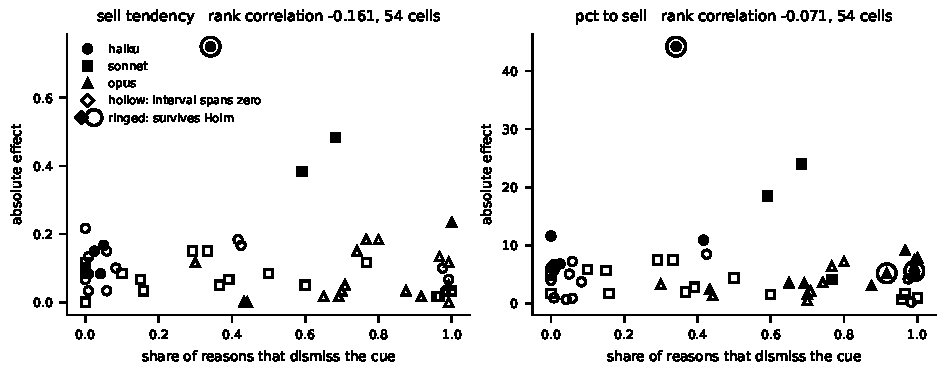
\includegraphics[width=\textwidth]{../figures/fig6_dissociation_acl.pdf}
  \caption{Dismissing the cue does not predict not acting on it. Each point
  is one model, effort and family cell: on the horizontal axis the share of
  that cell's one-sentence reasons that name the manipulated cue and discount
  it, on the vertical axis the size of that cell's effect, unsigned, because
  the claim is about magnitude. Only the six families the advisor ever refers
  to appear; the other three are never referred to at all, which the text
  takes up. If saying the right thing meant doing the right thing, the cloud
  would run downhill. The two Opus cells that survive Holm
  correction, at the right of the continuous panel, discount the cue in over
  nine tenths of their reasons and move with it anyway.}
  \label{fig:dissociation}
\end{figure*}
\else
\begin{figure}[t]
  \centering
  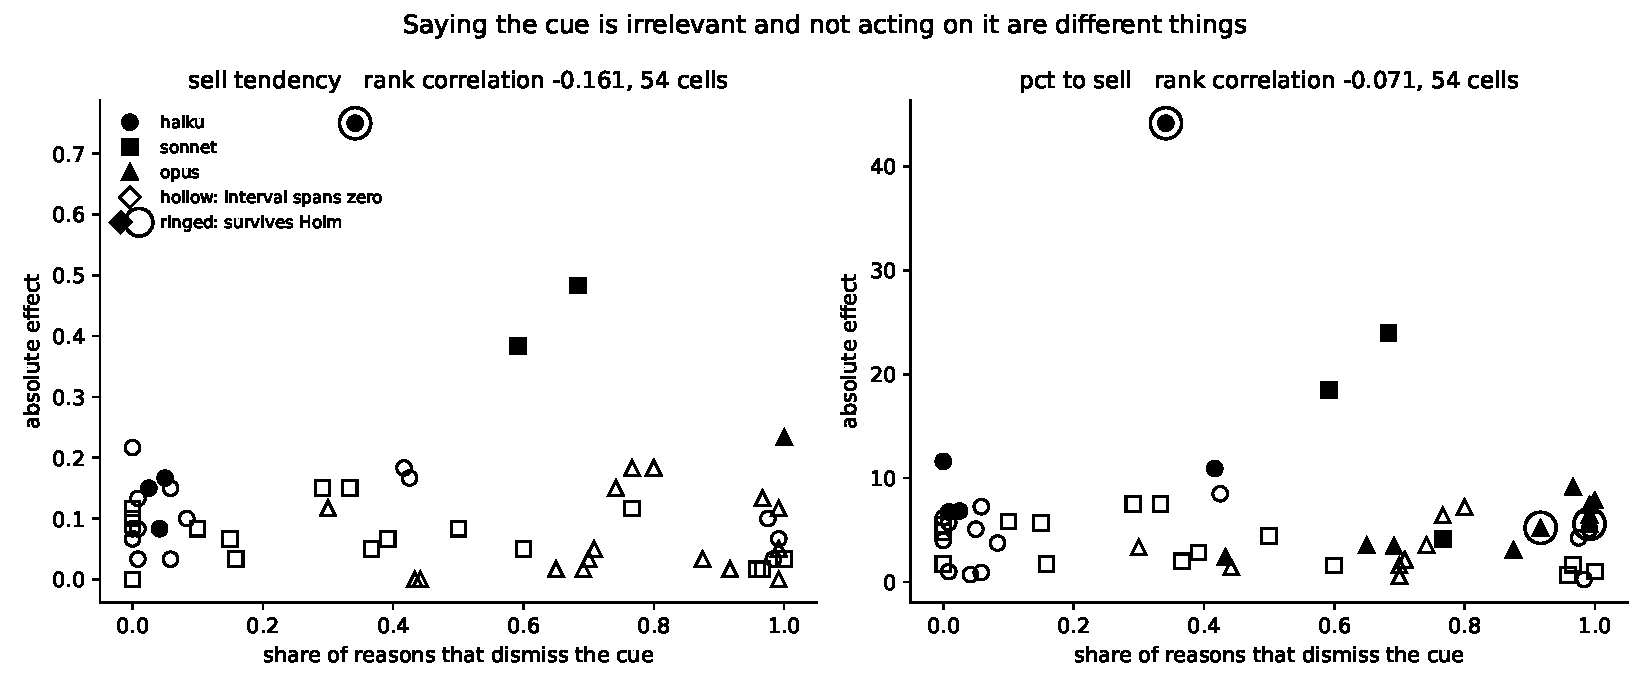
\includegraphics[width=\linewidth]{../figures/fig6_dissociation.pdf}
  \caption{Rejection rate against absolute effect, one point per model,
  effort and family cell, over the six families the advisor refers to. A flat
  cloud is the finding: the cells that discount the cue most are not the
  cells that move least.}
  \label{fig:dissociation}
\end{figure}
\fi


\paragraph{The dissociation.} Set the rejection rate of each cell against the
effect measured in that same cell, as Figure~\ref{fig:dissociation} does. If stated reasoning guarded against the
bias, a cell that discounts the cue in almost every reason it writes would
not move with it. Such cells exist, and they include the strongest results in
the study. Of 24 of 108 cells that discount the cue in at least 90\% of their
reasons, 7 of 24 still show an effect whose bootstrap interval excludes zero,
and 2 of 7 survive Holm correction across the whole family of tests. The two
that survive are Opus at \texttt{high} on anchoring, which discounts the
purchase price in 0.99 of its reasons and still shifts the recommended sale
by $+5.58$ percentage points \mbox{[$+2.83$, $+9.33$]}, $p_{\mathrm{Holm}} =
0.0189$; and Opus at \texttt{high} on mental accounting, which discounts the
accounting split in 0.92 of its reasons and still shifts it by $+5.22$
\mbox{[$+2.17$, $+8.97$]}, $p_{\mathrm{Holm}} = 0.0408$.

Only four cells in the entire study survive Holm correction, and they sit at
opposite ends of this scale. Two are the Opus cells above. The other two are
Haiku at \texttt{low} on disposition, on both measures, $p_{\mathrm{Holm}} =
0.0063$, a cell that discounts the cue in 0.34 of its reasons, the lowest
rate of any disposition cell in the design. The largest and most robust
effects in the study occur both where the model argues hardest against the
cue and where it argues least. For contrast, of the 30 of 108 cells that
essentially never name the cue, 6 of 30 show an effect clear of zero, which
is a similar share. Across all 54 nameable cells the rank correlation between
rejection rate and absolute effect is $-0.161$ on the categorical measure and
$-0.071$ on the continuous one: nothing, and if anything the wrong way. The
figure is the argument. A reader looking for the downhill cloud that stated
reasoning would produce will not find one.

\paragraph{What this does and does not establish.} The effort-to-rejection
result is identified, because the reasoning budget is set before the item is
seen. The rejection-to-bias association is not, and it fails for exactly the
reason this paper gives for declining to read Bini et al.'s self-reported
reasoning indicator as a treatment: the sentence and the recommendation are
produced in one forward pass, so neither is prior to the other and a third
property of the item can move both. What the dissociation supports is
narrower and still worth having. The explanation a model offers is not a
usable signal of whether that model was biased, because the cells where the
explanation most firmly rejects the cue are among the cells where the
behaviour most clearly follows it. An audit that reads the advisor's
reasoning and finds the right words in it has established that the right
words were produced.
\fi

\section{Discussion}
Three findings carry the paper, and they do not all point the same way.

\paragraph{The disposition effect is reversed, not absent.} These models are
more willing to recommend selling a position held below its cost basis than
one held above it, on both measures, where the pre-registered prediction
taken from the human literature was negative in both. Pooled over effort the
margin is wide in the two smaller models; in Opus it is indistinguishable
from zero, because the sign changes with effort, negative at \texttt{low} and
positive above it (\movedref{app:disposition}). This is the third independent measurement to point
this way, after \citet{malberg2025comprehensive} and
\citet{yee2026calibrating}, and the first under decision pressure with an
interval attached.

A model that is not loss averse is not thereby rational: it is differently
biased, in a way no human baseline anticipates, and the practical worry
inverts. Such an advisor will not help a client cling to losers; it may talk
them into realising losses they had no reason to realise, which in a taxable
account under a cash need is a real cost. The battery was not built to detect
that, so we offer it as the hypothesis this result generates, not one we
measured.

\paragraph{Reasoning effort reduces bias where there is bias to reduce, and
it works by compression.} H10 holds in every qualifying case, but the
count overstates the evidence: the shuffled label null for the pattern is
0.0125, not $2^{-9}$ (\movedref{sec:h10null}). What effort reliably
reduces is the spread of bias magnitudes across families, the largest effects
collapsing while the small ones hold or drift slightly upward. Whether the
mean falls with it depends on the model, detectably only in Opus. The
mechanism is uneven in the same direction (\movedref{sec:rtm}): in Haiku
the compression is large and survives both a correction for sampling error
and a placebo no shuffle of the effort labels reached, while in Opus the nine
families are not separable once item to item variation is charged against the
estimate, so there the falling spread is consistent with compression without
establishing it. The model giving the cleanest evidence for the mechanism is
therefore not the one giving the cleanest evidence for the reduction.

For deployment this is better news than a null and worse than it first
appears. Raising the budget intervenes on the recommendation and not only on
its justification, which is more than the ceiling account of
\citet{hu2026effort} predicts; but a practitioner should expect the
worst-behaved cue to improve substantially and the well-behaved ones little
or not at all. Effort lowers the ceiling on bias, it does not debias
generally.

\paragraph{Deliberation measured is not deliberation set.} The within-cell
relationship between generation length and bias is positive while the
between-cell relationship with the effort label is negative
(Section~\ref{sec:lengthorlabel}). Holding the item fixed resolves which
reading is right: the positive slope indexes item difficulty, because it
vanishes rather than reversing once the stimulus is fixed. The two quantities
cannot be used interchangeably, so work that infers a debiasing role for
deliberation from observed reasoning, the 40\% figure of
\citet{bini2026behavioral} included, identifies a different parameter from
the one an experimenter controls. Substituting one for the other on these
responses moves the headline from bias falling in six of six model by measure
combinations to one of nine cells, with the only interval excluding zero
pointing the wrong way. This is the most transferable result here and it
costs nothing to act on: set the budget exogenously wherever the parameter is
exposed.

The same gap opens between what these advisors say and what they do. A
detector over all 9{,}720 one-sentence reasons, hand validated at 138 of 138 on
rejections (\movedref{app:reasons}), finds that dismissal of the manipulated
cue rises with capability and effort yet does not predict the behaviour: of
the 24 of 108 cells that dismiss the cue in at
least 90\% of their reasons, 7 of 24 move with it anyway, among them both
Opus cells that survive Holm correction anywhere in the study, and the rank
correlation between dismissal rate and absolute effect across 54 cells is
$-0.161$ and $-0.071$. An audit that reads an advisor's explanation and finds
the right words has established that the right words were produced.

\ifsubmission
Two further notes are in Appendix~\ref{app:discnotes}. The pilot's reading
that deliberation substitutes for model capability does not survive the
confirmatory data: Opus has the steepest pooled effort slope and the only one
whose interval excludes zero on both measures, so effort did the most work in
the strongest model rather than the weakest. And all 86 responses whose two
measures contradict each other are Opus, 84 of them at \texttt{low} effort, a
failure of coherence rather than of bias whose fix was more effort.
\else
\label{sec:discnotes}\label{app:discnotes}
\paragraph{Where capability and deliberation sit.} The pilot suggested that
deliberation substitutes for model capability, with the weakest model gaining
most and the strongest having nothing left to gain. The confirmatory data do
not support that and we record the reversal rather than the original
reading. Opus has the steepest pooled effort slope and the only one whose
interval excludes zero on both measures. Effort did the most work in the
strongest model, not the weakest. The one place the substitution story does
hold is the single largest effect in the study, Haiku's disposition family,
which is where the pilot's reading came from; generalising from it was our
error, and the generalisation is what the full battery was for.

\paragraph{A note on coherence under a low budget.} All 86 responses whose
two measures contradict each other are Opus, and 84 are at \texttt{low}
effort. That is a different failure from bias: the model says hold and then
names a fraction of the position to sell. It is also the mechanism behind the
one cell that breaks the disposition sign pattern. For anyone deploying a
structured-output advisor, a low effort budget on a strong model bought
incoherence between fields at 2.59\% of responses, and the fix was more
effort, which took it to 0.06\%.

\fi

\ifsubmission\else\section{Limitations}
\label{sec:limitations}
% Keep these. Each one is a real constraint a reviewer will find anyway.

In the disposition family the percentage return is matched across the two
arms of each pair and the dollar amount is not. With the current price and
the share count held fixed, a position 50\% above its basis and one 50\%
below it cannot carry the same unrealised dollar amount. Percentage return is
the quantity the field measurement of the disposition effect is defined on
\citep{odean1998losses}, so it is the quantity matched here, but a model that
responds to dollar magnitude rather than to return would produce an effect in
this family that is not the disposition effect.

The brand salience family cannot claim normative invariance. A real ticker
carries the model's own knowledge of the company, so the two arms of those
pairs differ in information as well as in salience. Both arms use the real
company's sector so that the prompt is not self-contradictory, but the
remaining figures are synthetic in both, which a model with knowledge of the
company may notice. The family is reported separately and never pooled.

Companies in the seven confirmatory families are synthetic. This is
deliberate: \citet{lee2025yourai} report persistent model preferences over
specific real tickers, which would confound every manipulation here. The cost
is that the fundamentals are not real ones, and a model may treat an
unfamiliar name differently from a familiar one in ways the brand salience
family only begins to measure.

Effort is a vendor-defined control, not a measured quantity of reasoning.
\citet{hu2026effort} argue that it sets an upper budget on generation rather
than governing allocation, on a different model family and a different
outcome: they test GPT-OSS at three effort levels on reasoning tasks and
measure the alignment between generation length and human reaction times,
not whether a decision changes. Our token counts agree with their ceiling
claim, so the two results are not in conflict, and we claim an extension of
their manipulation to an outcome they did not measure rather than a
refutation of their finding. We report output token counts per cell so that the
treatment's effect on realised reasoning length is visible, but a null result
on H10 is consistent both with deliberation not reducing bias and with the
effort parameter not delivering the deliberation it nominally buys. These two
are separated only by the token counts, and we are explicit about that.


Synthetic scenarios are not real clients, and a willingness to recommend a
sale in a vignette is not a trade. Effects are prompt level and a different
phrasing of the same cue may move them. Model behaviour changes over time, so
these numbers are tied to the model IDs and run dates in Section~3.4, not to
the model families in general. The human baselines come from field studies of
brokerage accounts, a different instrument from this battery, so the
comparison is indicative rather than like for like. The brand salience and
price path families are exploratory. Twelve pairs per family is the binding
resolution limit of the design: it is what puts study-wide Holm correction out
of arithmetic reach (Section~\ref{sec:results}) and what leaves the
between-family spread in two of six cells indistinguishable from sampling
error (\movedref{sec:rtm}). An extension should add items per family
rather than trials per item. Nothing here is investment advice and
the author is not a licensed adviser.
\section{Ethics Statement}
No human subjects were involved and no personal, client or account data was
used. Every portfolio in the battery is generated by a released script from a
recorded seed, and the released response file contains model outputs only.

One exploratory family names real companies, Apple, Cisco, Johnson \&
Johnson and Procter \& Gamble, in order to vary brand familiarity while
holding the fundamentals fixed. Those fundamentals are invented, as they are
everywhere else in the battery. Nothing in the stimuli, the responses or this
paper is a statement about any real company's revenue, margins, balance sheet
or value, and the figures attached to those four names should not be read as
data about them.

The results point to a client-level harm that this battery was not built to
measure. A model whose disposition effect runs backwards is more willing to
recommend selling a position held below its cost basis, so in deployment it
would not help a client hold a losing position past the point of sense, but
it might recommend realising a loss the client had no reason to realise. In a
taxable account under a cash need that is a real cost. We state this as the
hypothesis our result generates, not as something we measured, because the
battery holds the tax treatment fixed and exempt by design.

The battery should not be used to certify a model as unbiased. Two findings
in this paper cut directly against that use. The nine cues here are not all
the cues an advisor faces, so a low score is evidence about these nine and
nothing more; and because reasoning effort compresses the spread of effects
rather than lowering them uniformly, a single mean taken at high effort will
understate how badly the worst cue still behaves. A reader selecting a model
on these grounds should read the per-family figures, not the mean.

No model was trained or fine-tuned. The whole study is inference: 9,720
requests through one vendor's batch API on the date recorded in
Section~\ref{sec:models}, under thirty US dollars in total. Model behaviour
changes with model versions, and the findings are tied to the identifiers
recorded there.

This paper was written with the assistance of a large language model, and
the assistant belongs to the family the paper measures. The analysis code,
the prose, and the labels of the reason text in \movedref{app:reasons} were all
produced that way, under the author's direction. A reader is entitled to
treat that as a conflict, and the answer to it is not a claim of
independence but an audit trail: every figure in the paper is printed by a
script in \texttt{analysis/}, the build refuses a manuscript containing a
number no script produced, and the 229 reason labels are committed beside
the text they label, so a reader who disagrees with a label can name it. The
responses themselves were produced by the batch API under the seeds and
identifiers recorded above, and no part of the measurement passed through
the assistant.

Nothing here is investment advice, and the author is not a licensed adviser.
\fi

\paragraph{What this does not settle.} Everything here is one vendor's
models, and the compression mechanism is the claim likeliest to be specific
to them, so the next step is a second model family exposing a comparable
parameter. What made the three answers of Section~\ref{sec:lengthorlabel}
separable at all was setting the budget before the model saw the item rather
than reading how hard it said it thought, and that is available wherever the
parameter is.

\paragraph{Reproducibility.} Prompts, generator seed, raw responses and analysis code are available at
\repourl. The pre-registration was committed before the first API call and
amended twice, both times before any model was queried. Every number here is
reproduced from the released response file by a deterministic script, named
in Appendix~\ref{app:repro}.

% Everything after this point is outside an ACL page limit.
\label{xbodyend}
% \pagetotal is only current once the page builder has run, so force it with
% a penalty in vertical mode. Without this the reading lags by whatever is
% still pending and stops moving when the body shrinks.
\par\penalty0
\makeatletter\message{^^JBODYFILL page=\thepage\space col=\if@firstcolumn 1\else 2\fi\space used=\the\pagetotal\space of=\the\pagegoal^^J}\makeatother
% ACL puts Limitations and the ethics statement after the body and before
% the references. Both sit after \label{xbodyend}, so neither counts
% against the page limit.
\ifsubmission\section{Limitations}
\label{sec:limitations}
% Keep these. Each one is a real constraint a reviewer will find anyway.

In the disposition family the percentage return is matched across the two
arms of each pair and the dollar amount is not. With the current price and
the share count held fixed, a position 50\% above its basis and one 50\%
below it cannot carry the same unrealised dollar amount. Percentage return is
the quantity the field measurement of the disposition effect is defined on
\citep{odean1998losses}, so it is the quantity matched here, but a model that
responds to dollar magnitude rather than to return would produce an effect in
this family that is not the disposition effect.

The brand salience family cannot claim normative invariance. A real ticker
carries the model's own knowledge of the company, so the two arms of those
pairs differ in information as well as in salience. Both arms use the real
company's sector so that the prompt is not self-contradictory, but the
remaining figures are synthetic in both, which a model with knowledge of the
company may notice. The family is reported separately and never pooled.

Companies in the seven confirmatory families are synthetic. This is
deliberate: \citet{lee2025yourai} report persistent model preferences over
specific real tickers, which would confound every manipulation here. The cost
is that the fundamentals are not real ones, and a model may treat an
unfamiliar name differently from a familiar one in ways the brand salience
family only begins to measure.

Effort is a vendor-defined control, not a measured quantity of reasoning.
\citet{hu2026effort} argue that it sets an upper budget on generation rather
than governing allocation, on a different model family and a different
outcome: they test GPT-OSS at three effort levels on reasoning tasks and
measure the alignment between generation length and human reaction times,
not whether a decision changes. Our token counts agree with their ceiling
claim, so the two results are not in conflict, and we claim an extension of
their manipulation to an outcome they did not measure rather than a
refutation of their finding. We report output token counts per cell so that the
treatment's effect on realised reasoning length is visible, but a null result
on H10 is consistent both with deliberation not reducing bias and with the
effort parameter not delivering the deliberation it nominally buys. These two
are separated only by the token counts, and we are explicit about that.


Synthetic scenarios are not real clients, and a willingness to recommend a
sale in a vignette is not a trade. Effects are prompt level and a different
phrasing of the same cue may move them. Model behaviour changes over time, so
these numbers are tied to the model IDs and run dates in Section~3.4, not to
the model families in general. The human baselines come from field studies of
brokerage accounts, a different instrument from this battery, so the
comparison is indicative rather than like for like. The brand salience and
price path families are exploratory. Twelve pairs per family is the binding
resolution limit of the design: it is what puts study-wide Holm correction out
of arithmetic reach (Section~\ref{sec:results}) and what leaves the
between-family spread in two of six cells indistinguishable from sampling
error (\movedref{sec:rtm}). An extension should add items per family
rather than trials per item. Nothing here is investment advice and
the author is not a licensed adviser.
\section{Ethics Statement}
No human subjects were involved and no personal, client or account data was
used. Every portfolio in the battery is generated by a released script from a
recorded seed, and the released response file contains model outputs only.

One exploratory family names real companies, Apple, Cisco, Johnson \&
Johnson and Procter \& Gamble, in order to vary brand familiarity while
holding the fundamentals fixed. Those fundamentals are invented, as they are
everywhere else in the battery. Nothing in the stimuli, the responses or this
paper is a statement about any real company's revenue, margins, balance sheet
or value, and the figures attached to those four names should not be read as
data about them.

The results point to a client-level harm that this battery was not built to
measure. A model whose disposition effect runs backwards is more willing to
recommend selling a position held below its cost basis, so in deployment it
would not help a client hold a losing position past the point of sense, but
it might recommend realising a loss the client had no reason to realise. In a
taxable account under a cash need that is a real cost. We state this as the
hypothesis our result generates, not as something we measured, because the
battery holds the tax treatment fixed and exempt by design.

The battery should not be used to certify a model as unbiased. Two findings
in this paper cut directly against that use. The nine cues here are not all
the cues an advisor faces, so a low score is evidence about these nine and
nothing more; and because reasoning effort compresses the spread of effects
rather than lowering them uniformly, a single mean taken at high effort will
understate how badly the worst cue still behaves. A reader selecting a model
on these grounds should read the per-family figures, not the mean.

No model was trained or fine-tuned. The whole study is inference: 9,720
requests through one vendor's batch API on the date recorded in
Section~\ref{sec:models}, under thirty US dollars in total. Model behaviour
changes with model versions, and the findings are tied to the identifiers
recorded there.

This paper was written with the assistance of a large language model, and
the assistant belongs to the family the paper measures. The analysis code,
the prose, and the labels of the reason text in \movedref{app:reasons} were all
produced that way, under the author's direction. A reader is entitled to
treat that as a conflict, and the answer to it is not a claim of
independence but an audit trail: every figure in the paper is printed by a
script in \texttt{analysis/}, the build refuses a manuscript containing a
number no script produced, and the 229 reason labels are committed beside
the text they label, so a reader who disagrees with a label can name it. The
responses themselves were produced by the batch API under the seeds and
identifiers recorded above, and no part of the measurement passed through
the assistant.

Nothing here is investment advice, and the author is not a licensed adviser.
\fi

\ifsubmission\else\bibliographystyle{plainnat}\fi
\bibliography{refs}

\appendix

% The battery table is a longtable, which cannot be set in a two column
% document, and splitting a 108 row table across columns would make the
% matched pairs unreadable anyway. \onecolumn starts the appendix on a fresh
% page and sets it full width. In the single column reading build the command
% is a no-op, so both builds use this file unchanged.
% Sections moved out of the body for the submission build. Nothing is cut:
% in the single column reading build every one of these appears inline where
% it was written, and this block is empty. The page limit at an ACL venue
% covers the body only, so material that a reader needs but a reviewer can
% reach by reference belongs here rather than on the cutting room floor.
\ifsubmission
\section{Two schema limits}
\movedhead{Two schema limits}
\label{sec:schemalimits}\label{app:schemalimits}
Two schema limits are worth recording for anyone reproducing this. The API
rejects \texttt{minimum} and \texttt{maximum} on a numeric field with an
HTTP 400, so the stated 0 to 100 bounds are advisory and are checked at
collection rather than by the schema. A value outside them is flagged and
never clamped, because clamping would convert a failure to follow the
instruction into a valid looking extreme answer. It is then dropped from the
continuous measure, since a number outside 0 to 100 is not a percentage of a
position and cannot enter a mean of percentages, while the same response's
categorical answer is retained. The two measures therefore rest on slightly
different numbers of observations, and both counts are reported. The
categorical and continuous measures can also disagree, for instance
\texttt{HOLD} with a non-zero percentage. Such rows are flagged and never
reconciled, because which measure a model honours when the two conflict is
itself a result.


\section{Sonnet's medium cell}
\movedhead{Sonnet's medium cell}
\label{sec:sonnetmedium}\label{app:sonnetmedium}
One cell is an exception worth isolating now, because several later results
depend on it. Sonnet's \texttt{medium} cell is not a distinct treatment
level. It generates 163.4 mean output tokens against 160.1 at \texttt{low}, a
standardised difference of $d = 0.06$, where every other adjacent contrast in
every model is near or above $d = 1$. Its within-item entropy agrees, 0.053
bits against 0.054, and so does its within-item share of variance, 4.6\%
against 4.5\%. On three independent measures Sonnet's \texttt{medium} cell is
a second copy of its \texttt{low} cell.


\section{Bias incidence in detail}
\movedhead{Bias incidence in detail}
\label{sec:incidence}\label{app:incidence}
Four cells clear Holm correction within their model and effort cell: Haiku at
\texttt{low} effort on the disposition family, on both measures, at $+0.750$
$[+0.483, +1.033]$ and $+44.167$ $[+28.500, +59.750]$; and Opus at
\texttt{high} effort on anchoring at $+5.583$ $[+2.833, +9.333]$ and on
mental accounting at $+5.217$ $[+2.167, +8.967]$, both on the continuous
measure. All four survive every one of their twelve leave-one-pair-out refits
with an interval that still excludes zero, so none of them rests on a single
item.

Nothing survives a correction applied across all 81 cells at once, and that
is a statement about resolution rather than about the effects: the smallest
$p$ anywhere is 0.0007, the most significant of 81 tests would need to clear
0.000617, and with twelve pairs the sign flipping test cannot return a $p$
below 0.00049 at any effect size. A study-wide Holm survivor is out of reach
by arithmetic here, and the pre-registered decision rule is the interval,
which multiplicity does not touch.


\section{The pooled disposition figure, by model}
\movedhead{The pooled disposition figure, by model}
\label{sec:disposition}\label{app:disposition}
The abstract states the disposition reversal once, over the whole study,
because the direction is a claim about these models rather than about one
cell of a design that varies model and effort. That pooling is a secondary
aggregation and not a registered quantity, and it is not uniform across the
three models. The figures below come from \texttt{analysis/aggregate.py},
which imports the bootstrap, the seed and the matched pair definition from
the registered script and changes only the grouping.

\begin{table}[t]
  \centering
  \footnotesize
  \begin{tabular}{lrl}
    \toprule
                     & Effect & 95\% CI \\
    \midrule
    \multicolumn{3}{l}{\textit{Categorical, sell tendency}} \\
    Haiku            & $+0.367$  & $[+0.211, +0.533]$ \\
    Sonnet           & $+0.328$  & $[+0.172, +0.494]$ \\
    Opus             & $+0.022$  & $[-0.106, +0.144]$ \\
    All three pooled & $+0.239$  & $[+0.148, +0.331]$ \\
    \midrule
    \multicolumn{3}{l}{\textit{Continuous, percentage points}} \\
    Haiku            & $+21.194$ & $[+12.722, +30.389]$ \\
    Sonnet           & $+15.556$ & $[+8.111, +23.667]$ \\
    Opus             & $+3.378$  & $[-2.567, +9.350]$ \\
    All three pooled & $+13.376$ & $[+8.826, +18.037]$ \\
    \bottomrule
  \end{tabular}
  \caption{The disposition family pooled over effort, by model, and over
  both factors. Positive is the reversal: more willing to sell the position
  held below its cost basis. Each model rests on 36 matched pairs and the
  pooled row on 108. Produced by \texttt{analysis/aggregate.py}, which
  verifies itself against the registered per-cell figures before reporting.}
  \label{tab:disposition}
\end{table}

Two of the three models carry the reversal with an interval clear of zero on
both measures. Opus does not, and the reason is not that Opus is unbiased on
this family. Its effect changes sign as effort rises: on the continuous
measure it runs $-6.417$ at \texttt{low}, $+9.133$ at \texttt{medium} and
$+7.417$ at \texttt{high}, and on the categorical measure $-0.183$, $+0.133$
and $+0.117$. Pooling over effort averages one negative cell against two
positive ones and returns almost nothing. The absolute effect still falls
monotonically, which is what H10 asserts, so these cells are among the nine
qualifying falls; the fall simply passes through zero instead of stopping
short of it. At \texttt{low} effort Opus is the one cell in the study that
points the human way on this family, and it is also the only model whose
disposition sign the manipulation moves.

The practical reading is that the reversal is a property of these two
models at every effort level and of the third at two of three, and that a
single pooled number is the wrong instrument for a quantity the design was
built to split. It is reported because the abstract quotes it, and a figure
in an abstract should be traceable to the grouping that produced it. The
registered unit of analysis is the cell, in Figure~\ref{fig:forest} and the
per-cell tables.


\section{The nine qualifying cases}
\movedhead{The nine qualifying cases}
\label{sec:h10cases}\label{app:h10cases}
Four of the seven confirmatory families qualify for H10 on the categorical
measure and five on the continuous measure. On the
categorical measure they are Haiku and Sonnet on disposition, falling from
$+0.750$ to $+0.167$ and from $+0.383$ to $+0.117$, and Opus on framing and
anchoring, from $+0.300$ to $+0.017$ and from $+0.233$ to $+0.050$. On the
continuous measure they are Haiku on disposition and home bias, from
$+44.167$ to $+8.500$ and from $+11.617$ to $+4.000$, Sonnet on disposition,
from $+18.500$ to $+4.167$, and Opus on framing and anchoring, from $+15.167$
to $+1.750$ and from $+7.833$ to $+5.583$.


\section{Two further notes on the findings}
\label{sec:discnotes}\label{app:discnotes}
\paragraph{Where capability and deliberation sit.} The pilot suggested that
deliberation substitutes for model capability, with the weakest model gaining
most and the strongest having nothing left to gain. The confirmatory data do
not support that and we record the reversal rather than the original
reading. Opus has the steepest pooled effort slope and the only one whose
interval excludes zero on both measures. Effort did the most work in the
strongest model, not the weakest. The one place the substitution story does
hold is the single largest effect in the study, Haiku's disposition family,
which is where the pilot's reading came from; generalising from it was our
error, and the generalisation is what the full battery was for.

\paragraph{A note on coherence under a low budget.} All 86 responses whose
two measures contradict each other are Opus, and 84 are at \texttt{low}
effort. That is a different failure from bias: the model says hold and then
names a fraction of the position to sell. It is also the mechanism behind the
one cell that breaks the disposition sign pattern. For anyone deploying a
structured-output advisor, a low effort budget on a strong model bought
incoherence between fields at 2.59\% of responses, and the fix was more
effort, which took it to 0.06\%.


\section{The budget and the behaviour are not the same variable}
% No \movedhead here, unlike the other moved sections. body.tex prints this
% heading in both builds, because sec:mediator and sec:lengthorlabel are
% referenced from shared prose and so have to resolve to a Section in both.
% A \movedhead as well set the title twice in the reading build, as an empty
% subsection followed by the real one.
\label{app:mediator}
The argument for setting the reasoning budget through the API rather than
measuring how much reasoning a response contains is made in
Section~\ref{sec:deliberation} on identification grounds: a measure read off
the response is produced by the same forward pass as the answer, so it cannot
separate reasoning that helped from reasoning that a hard item provoked. This
data can test that argument instead of asserting it, because it holds both
variables. The effort parameter is exogenous, set before the model sees the
item. Output tokens are endogenous, chosen by the model for each response.
They are not the self-reported analytical-reasoning indicator used by
\citet{bini2026behavioral}, but they are the same class of variable: a
within-cell, model-chosen measure of how much reasoning a response contains,
with no experimental control over it. None of this subsection is
pre-registered; it was written after the data were in hand.

The parameter does set reasoning volume, so the two variables are not
measuring different constructs. Output tokens rise from \texttt{low} to
\texttt{high} by a factor of 2.33 in Haiku, 2.44 in Opus and 2.91 in Sonnet,
and the distributions barely overlap: 0.1\% of Haiku's and Opus's
\texttt{low} effort responses exceed the median \texttt{high} effort
response, 0.0\% of Sonnet's, and in the other direction 0.0\%, 0.0\% and
3.5\%. If an observational measure of reasoning volume recovers the causal
effect of reasoning volume anywhere, it should do so here.

It does not. \texttt{analysis/mediator.py} runs the paper's own arithmetic
three ways on the same 9{,}720 responses, with the same families, items and
statistics, changing only which responses enter each pair mean.

\paragraph{Exogenous.} Comparing effort levels, the mean absolute family
effect falls from \texttt{low} to \texttt{high} in all three models on both
measures, by $-0.120$, $-0.069$ and $-0.050$ on the categorical measure for
Opus, Sonnet and Haiku, and by $-2.628$, $-3.667$ and $-3.700$ on the
continuous one. Six of six.

\paragraph{Endogenous, between items.} Within a single model and effort cell
the effort label is constant, but generation length still varies widely from
item to item. If deliberation itself is what reduces bias, then holding the
label fixed, pairs on which the model happened to generate more should show
less bias. They show more. The Spearman correlation between a pair's mean
output tokens and its absolute effect, pooled across all nine cells with the
cell means removed from both variables so that only within-cell variation
contributes, is $+0.190$ ($p = 0.0001$) on the categorical measure and
$+0.154$ ($p = 0.0001$) on the continuous measure, over 972 pairs. The
relationship is positive in 17 of the 18 cell by measure combinations and
reaches $p < 0.05$ in eight of them. Taken as a median split instead, so that
the statistic matches the one used for the exogenous comparison, the mean
absolute effect is lower in the heavier half in one cell of nine on both
measures, and pooled over effort and bootstrapped over pairs the contrast is
positive in all three models on both measures, with Haiku on the categorical
measure excluding zero in the wrong direction at $+0.066$ $[+0.014, +0.143]$.
Between cells, bias falls as effort rises. Within cells, bias rises with
length. The two slopes have opposite signs.

\paragraph{Endogenous, within item.} Two readings of that reversal were
available. The first is that the exogenous budget and the model's own
allocation of tokens are distinct interventions with distinct effects. The
second is reverse causation: an item that provokes bias also provokes a
longer answer, so length is an index of item difficulty rather than of
deliberation. A third design separates them. Inside one model by effort cell,
split the five trials of each single item at that item's own median token
count. The stimulus, the family, the company and the effort setting are then
identical across the split, and only the model's sample to sample choice of
how much to write differs. The reversal disappears and nothing takes its
place: the mean absolute effect falls in four of nine cells, which is what
chance gives, and every pooled interval contains zero, the largest being
$-0.585$ $[-2.896, +1.999]$ for Haiku on the continuous measure. The positive
association is therefore a property of the item, not of the response, and the
difficulty reading is the one the data support.

An observational study of these responses would thus have reported that
reasoning makes the bias worse, or that it does nothing, depending on whether
it conditioned on the item. The experiment reports that it reduces the bias,
in every model and on both measures.

Leverage rules out the obvious objection that the observational designs
simply had less variation to work with. Both separate their halves by a
similar amount, 49.5 and 53.6 output tokens in Opus, 59.6 and 61.2 in Sonnet,
132.0 and 155.1 in Haiku, which is between 0.19 and 0.39 of the gap the
parameter opens. The two observational designs therefore have the same
leverage as each other and less than the experiment. Less leverage is a fair
explanation of the within-item null, which should be read as consistent with
low power rather than as evidence against the experiment. It is not an
explanation of a sign reversal. Where the between-item design returns the
wrong sign it is returning confounding, not noise.

Because the two observational designs differ only in whether the item is held
fixed, their disagreement locates that confounding in the item, and two item
level properties move with the token count. Harder items draw more words and
are more bias-prone, which is the reading above. The second is visible in the
data and is less often named: the families themselves differ in how much the
model writes about them, so splitting on tokens re-weights the cues being
averaged. Mental accounting contributes 75.5\% of its responses to the heavy
half and price path 68.2\%, while action bias contributes 28.0\% and framing
30.2\%. A measure of reasoning volume taken from the response is therefore
also a measure of which cue was present.

What no observational design here can remove is the loop that motivates the
study. A response's recommendation and the length of its justification are
produced together, so conditioning on length conditions on the answer.
Setting the budget before the item is seen is the only one of the three
designs that avoids this, and it is the only one that recovers an effect. A
design which measures deliberation by observing the model, whether through
generated length or through the model's own report of its reasoning, is
measuring a quantity whose association with bias runs the other way from the
one an experimenter can set. That is not a refinement of the identification
problem in \citet{bini2026behavioral}; it is a demonstration of it. It is not
a demonstration that their finding is wrong: their mediator, items and models
all differ from these. It shows that the class of design cannot be relied on
to recover the sign, which is a claim about method and not about their
result.


\section{What the advisor says about the cue}
\movedhead{What the advisor says about the cue}
\label{app:reasons}

Every response carries a one-sentence \texttt{one\us sentence\us reason}, and
the study has 9{,}720 of them. They are the only direct evidence in the
dataset about what the model was attending to, and they bear on a question
the design cannot otherwise reach: whether an advisor that is moved by a cue
is an advisor that failed to notice it.

\paragraph{The measure.} For each of the six families whose manipulation
puts a nameable object in the prompt, a cue pattern asks whether the reason
refers to that object at all, and a second set of patterns asks whether it
refers to it in order to discount it. A reason is \emph{silent} if it never
mentions the cue, \emph{cites} it if it mentions it as a consideration, and
\emph{rejects} it if it names the cue and sets it aside. Word order carries
most of the work, because it is the only thing separating a rejection from
its opposite: ``on current merits rather than the prior peak'' discounts the
peak, while ``sell 10\% rather than 20\%, given the prior peak'' does not,
and the two differ in no word that a bag of markers would see. Rejection markers
are therefore split into a symmetric set and two directional sets, and
proximity rather than presence decides, inside a 90-character window either
side of the cue.

\paragraph{Validation.} A regex measure of this kind is worth nothing
unvalidated, so four rounds of reasons were drawn and hand labelled, each
under its own seed and disjoint from the rounds before it: 60, 60, 55 and 54
reasons, 229 in all, stratified so that each family contributes four reasons
the detector called a rejection and three from each of the other two states.
Only the fourth round is validation. The first reading of each of the two
middle rounds exposed a defect in the patterns rather than a limit of the
measure, and repairing a round against its own labels spends it; the first
round was tuning from the start. The labels are committed with the reason
text beside them, so a disagreement with any of them is a reviewable claim
rather than a private judgement.

The first defect is worth stating, because it is the kind of error that
survives every test a project of this size would normally run. The patterns
were written with \texttt{re.VERBOSE} for legibility, and
\texttt{re.VERBOSE} strips unescaped whitespace from the pattern, so
\texttt{purchase price} compiled to \texttt{purchaseprice} and matched
nothing. Every multi-word phrase in the file was inert, which held every
rejection rate it printed at roughly a third of its true value, and the
tables it produced were internally consistent and entirely wrong. Nothing
found it but reading the sample by hand.

On the final round the detector's precision on rejections is 1.000, and
across all four rounds it is 138 of 138: it has never once called a rejection
that the hand label did not confirm, in any family. Recall is 0.667 in that
sample and 0.857 once each stratum is reweighted by how many reasons it holds
in the corpus, the difference being that the draw deliberately oversamples
the two strata where the misses live. Every rejection rate below is therefore
a floor, and the floor sits roughly a seventh under the rate. Recall on the
validation round is 0.632 for Opus, 0.750 for Sonnet and 0.600 for Haiku,
against measured rejection rates that span 0.76 to 0.25, so the ordering
across models is not a property of the patterns.

\paragraph{Three manipulations nothing refers to.} The other three families
manipulate how the decision is framed rather than what is in it, and under
patterns written to be as generous as possible the reasons almost never refer
to the manipulation: 2 of 1{,}080 reasons in framing, 1 of 1{,}080 in
action bias, and 0 of 1{,}080 in brand salience. This is not a failure of the
measure. These manipulations leave no object in the prompt for a sentence to
name, which is what makes them structural, and two of the three still move
the recommendation. A cue does not have to be available to the explanation
in order to change the answer.

\paragraph{Rejection tracks capability and effort.} Over the six nameable
families, Opus discounts the cue in 0.72, 0.77 and 0.79 of its reasons at
\texttt{low}, \texttt{medium} and \texttt{high}; Sonnet in 0.39, 0.41 and
0.50; Haiku in 0.23, 0.25 and 0.26. Per family and model, 12 of 18
combinations reject more at \texttt{high} than at \texttt{low}, 7 of 18 with
a bootstrap interval excluding zero. So effort does buy more of the thing
that looks like debiasing, and unlike the behavioural effects this is
identified: effort is set through the API before the model sees the item.

Two families show the ends of the range. Anchoring is discounted by every
model at every effort, between 0.96 and 1.00 of the time: the purchase price
is recognised as irrelevant essentially always. Home bias is discounted by
Opus in 0.30 to 0.44 of its reasons and by Sonnet and Haiku in almost none,
0.00 at all three efforts for Sonnet and 0.00, 0.01 and 0.00 for Haiku. The
smaller models do not argue that the foreign listing is irrelevant; they
never raise it.

\ifsubmission
\begin{figure*}[t]
  \centering
  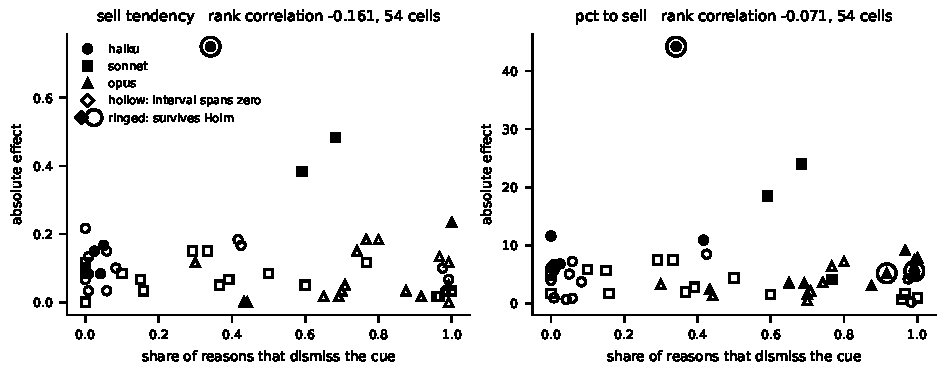
\includegraphics[width=\textwidth]{../figures/fig6_dissociation_acl.pdf}
  \caption{Dismissing the cue does not predict not acting on it. Each point
  is one model, effort and family cell: on the horizontal axis the share of
  that cell's one-sentence reasons that name the manipulated cue and discount
  it, on the vertical axis the size of that cell's effect, unsigned, because
  the claim is about magnitude. Only the six families the advisor ever refers
  to appear; the other three are never referred to at all, which the text
  takes up. If saying the right thing meant doing the right thing, the cloud
  would run downhill. The two Opus cells that survive Holm
  correction, at the right of the continuous panel, discount the cue in over
  nine tenths of their reasons and move with it anyway.}
  \label{fig:dissociation}
\end{figure*}
\else
\begin{figure}[t]
  \centering
  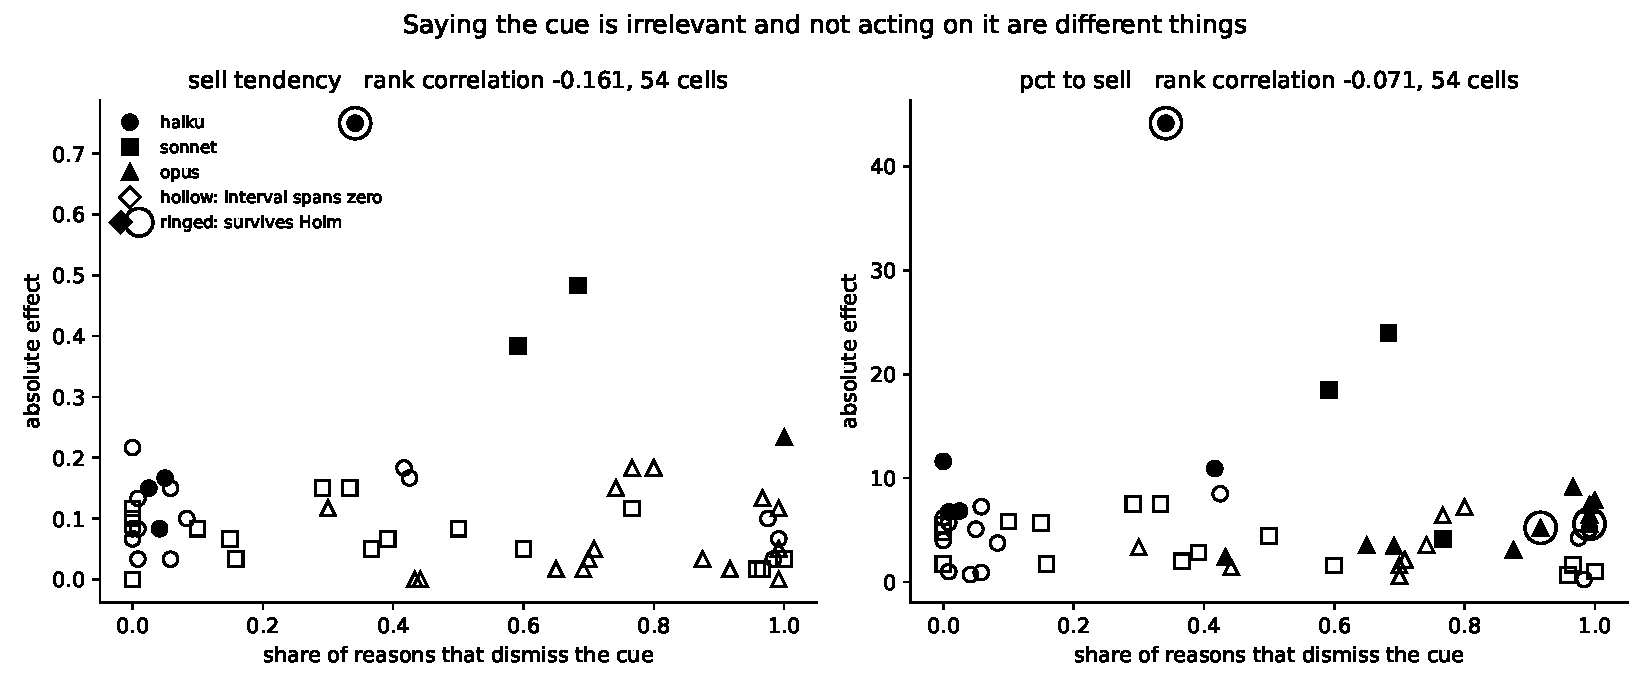
\includegraphics[width=\linewidth]{../figures/fig6_dissociation.pdf}
  \caption{Rejection rate against absolute effect, one point per model,
  effort and family cell, over the six families the advisor refers to. A flat
  cloud is the finding: the cells that discount the cue most are not the
  cells that move least.}
  \label{fig:dissociation}
\end{figure}
\fi


\paragraph{The dissociation.} Set the rejection rate of each cell against the
effect measured in that same cell, as Figure~\ref{fig:dissociation} does. If stated reasoning guarded against the
bias, a cell that discounts the cue in almost every reason it writes would
not move with it. Such cells exist, and they include the strongest results in
the study. Of 24 of 108 cells that discount the cue in at least 90\% of their
reasons, 7 of 24 still show an effect whose bootstrap interval excludes zero,
and 2 of 7 survive Holm correction across the whole family of tests. The two
that survive are Opus at \texttt{high} on anchoring, which discounts the
purchase price in 0.99 of its reasons and still shifts the recommended sale
by $+5.58$ percentage points \mbox{[$+2.83$, $+9.33$]}, $p_{\mathrm{Holm}} =
0.0189$; and Opus at \texttt{high} on mental accounting, which discounts the
accounting split in 0.92 of its reasons and still shifts it by $+5.22$
\mbox{[$+2.17$, $+8.97$]}, $p_{\mathrm{Holm}} = 0.0408$.

Only four cells in the entire study survive Holm correction, and they sit at
opposite ends of this scale. Two are the Opus cells above. The other two are
Haiku at \texttt{low} on disposition, on both measures, $p_{\mathrm{Holm}} =
0.0063$, a cell that discounts the cue in 0.34 of its reasons, the lowest
rate of any disposition cell in the design. The largest and most robust
effects in the study occur both where the model argues hardest against the
cue and where it argues least. For contrast, of the 30 of 108 cells that
essentially never name the cue, 6 of 30 show an effect clear of zero, which
is a similar share. Across all 54 nameable cells the rank correlation between
rejection rate and absolute effect is $-0.161$ on the categorical measure and
$-0.071$ on the continuous one: nothing, and if anything the wrong way. The
figure is the argument. A reader looking for the downhill cloud that stated
reasoning would produce will not find one.

\paragraph{What this does and does not establish.} The effort-to-rejection
result is identified, because the reasoning budget is set before the item is
seen. The rejection-to-bias association is not, and it fails for exactly the
reason this paper gives for declining to read Bini et al.'s self-reported
reasoning indicator as a treatment: the sentence and the recommendation are
produced in one forward pass, so neither is prior to the other and a third
property of the item can move both. What the dissociation supports is
narrower and still worth having. The explanation a model offers is not a
usable signal of whether that model was biased, because the cells where the
explanation most firmly rejects the cue are among the cells where the
behaviour most clearly follows it. An audit that reads the advisor's
reasoning and finds the right words in it has established that the right
words were produced.


\section{The nine families with their normative justification}
\label{app:hypothesesfull}
% table* spans both columns in the two column build and degrades to an
% ordinary full width table in the single column one, so the widths below
% work in both. In a single ACL column this table overflows by 158pt, which
% is not fixable by shrinking the font.
\begin{table*}[t]
  \centering
  \small
  \setlength{\tabcolsep}{4pt}
  \begin{tabular}{@{}p{2.5cm}p{3.0cm}p{6.9cm}cc@{}}
    \toprule
    Family & Cue varied & Why the recommendation should not change
           & Pred. & Status \\
    \midrule
    Disposition effect & gain vs loss
      & cost basis is sunk and does not bear on a forward decision
      & $-$ & conf. \\
    Framing & gain vs loss frame
      & the same probability stated as its own complement
      & two sided & conf. \\
    Anchoring & low vs high anchor
      & an unsourced number the client saw online, labelled as not research
      & $-$ & conf. \\
    Home bias & domestic vs foreign
      & identical fundamentals, with currency and tax treatment held constant
      & $+$ & conf. \\
    Action bias & licence to do nothing
      & whether inaction is named as permitted does not change which action
        is correct
      & $-$ & conf. \\
    Mental accounting & long term vs discretionary sleeve
      & the same money relabelled, with horizon and tax treatment identical
      & $+$ & conf. \\
    Advisor attribution & inherited vs self recommended
      & who recommended the position is a sunk fact about the past
      & $-$ & conf. \\
    Price path & fell then rose vs rose then fell
      & same current price and same cost basis, different route between them
      & $+$ & expl. \\
    Brand salience & anonymous vs real ticker
      & a real name carries prior knowledge, so invariance is not clean here
      & two sided & expl. \\
    \bottomrule
  \end{tabular}
  \caption{The nine bias families, with the normative reason the recommendation should not change. Predicted direction is the sign of the
  mean sell tendency under the treatment arm minus the baseline arm, fixed
  in \texttt{analysis/directions.py} before the run. Advisor attribution and
  price path are original to this study.}
  \label{tab:hypothesesfull}
\end{table*}


\section{Companies and randomisation}
\movedhead{Companies and randomisation}
\label{sec:companies}\label{app:companies}
Company profiles are synthetic. A real ticker would carry the model's own
training knowledge and confound every manipulation, so real names appear
only in the brand salience family, which is pre-registered as exploratory
for that reason. Twelve profiles span sectors and are deliberately mixed on
fundamentals, so neither buying nor selling is obviously correct, which is
what makes the decision pressure of Section~\ref{sec:pressure} necessary
rather than optional. Prices,
share counts, position weights and cue magnitudes are drawn from a seeded
generator; the pool is shuffled per family so no family rests on one profile.


\section{Human findings and the family built from each}
\movedhead{Behavioural biases in human investors}
\label{app:humaninvestors}
The biases this paper tests are not hypotheses about language models. They
are documented regularities in human investors, and the design borrows their
operationalisations rather than inventing new ones. Prospect theory
\citep{kahneman1979prospect} supplies the reference dependence that makes a
cost basis matter at all, and the framing manipulations of
\citet{tversky1981framing} supply the form of the framing family here: the
same information, valenced two ways. The disposition effect was named by
\citet{shefrin1985disposition} as a reluctance to realise losses and measured
in brokerage account data by \citet{odean1998losses}, who scores which
positions investors sell when they sell something. Mental accounting
\citep{thaler1985mental} motivates the sleeve manipulation, myopic loss
aversion \citep{benartzi1995myopic} the evaluation horizon, and home bias
\citep{french1991homebias} the domestic and foreign arms.
\citet{barber2000hazardous} supply the reason any of this is worth
measuring in an advisor: these biases carry a cost in realised returns.

These are also the source of the human baselines in
Section~\ref{sec:humanbaselines}, and the comparison is indicative rather
than like for like, because a field study of brokerage accounts and a
prompt battery are different instruments.
% Closed 2026-10-26. The Odean rates in Section 4.2 are read from Table I on
% p.1783 of the primary paper, not from any summary of it. Any further human
% rate added later must clear the same bar.


\section{The prompt-level treatments of \citet{bini2026behavioral}}
% Printed inline in the reading build and as an appendix section in the
% submission build, so it is worded to stand on its own either way.
\label{app:deliberation}
\citet{bini2026behavioral} treat the model at the prompt level throughout.
Priming it to act as a rational investor under expected utility does reduce
bias, at a magnitude they call economically modest, while supplying a
four-step expected utility procedure is ineffective, and supplying the
findings of \citet{kahneman1979prospect} lowers rational responses by about
29\%. Their own summary is that debiasing remains a challenging task.


\section{Decision pressure and the pilot that forced it}
\movedhead{Decision pressure}
\label{sec:pressure}\label{app:pressure}
Every item states that the client must raise cash equal to 10\% of the
account this month, and that the account is tax exempt so no sale carries a
tax consequence. Both sentences are identical across the arms of a pair.
Neither is cosmetic.

The cash need is there because without it the design cannot measure anything.
In a pilot of 108 requests spanning all nine families and all three models,
93\% of responses were \texttt{HOLD}, with no instance of \texttt{BUY\_MORE}
and none of \texttt{SELL\_ALL}. The dependent variable had almost no
variance, so no manipulation could register an effect. Two candidate
explanations were tested and both failed: removing a normative instruction
from the system prompt left the distribution unchanged at 83\% \texttt{HOLD},
and adding a continuous target portfolio weight produced the position's
current weight, to the decimal, in 28 of 36 responses. The cause was the
stimulus. Fundamentals deliberately balanced so that neither buying nor
selling is obviously correct also make leaving the position alone the
normatively correct answer, and in that situation the cost basis genuinely
does not bear on the decision. There is no decision to bias. Human
disposition effect experiments do not have this problem because they always
require a realisation choice: \citet{odean1998losses} measures which
positions investors sell \emph{when they sell something}. With the cash need
in place, \texttt{HOLD} fell to 71\% and the continuous measure acquired real
spread (mean 15.3, sd 25.2, non-zero in 124 of 432 responses). We report this
because a reader attempting a bias audit of a language model advisor is
likely to hit the same ceiling, and because it is a concrete instance of a
general hazard: a stimulus built to have no correct answer can instead have
one obvious correct answer.

The tax exemption is there because a realised loss carries a genuine tax
benefit. Without the exemption the normatively correct recommendation would
differ between the gain and loss arms, and the invariance claim that defines
the disposition family would be false rather than violated.

\ifsubmission
One response format was tested and rejected. Asked to choose between two
positions identical but for cost basis, the model picked the same one 24
times out of 24, which reads as a large preference; given a continuous
allocation over those same two positions it answered exactly 50.0 every
time, with zero variance. The apparent effect was an artefact of forcing a
binary choice on a model that had already seen the options were equivalent.
Appendix~\ref{app:rejected} gives the full exchange, because the failure mode
generalises to any forced-choice bias probe.
\else
\movedhead{A format that was rejected}
\label{sec:rejected}\label{app:rejected}
A forced choice between a winner and a loser is the canonical
operationalisation of the disposition effect. Asked to raise cash by selling
either position A or position B, identical but for cost basis, the model
chose A in 24 of 24 trials irrespective of which position was the winner,
which presents as a large position preference. Offered a continuous
allocation over the same two positions, all 72 responses answered exactly
50.0 with zero variance. The apparent preference was an artifact of forcing a
binary choice on a model that had correctly identified the options as
equivalent, and is reported here as a warning about binary forced choice
items rather than as a finding about order effects. No forced binary choice
appears anywhere in the study.

The two asset format is not a straw man: it is what the largest audit in this
area uses. \citet{malberg2025comprehensive} present two owned assets, one up
and one down, ask which the model would rather sell, and swap which asset has
gained between the control and treatment arms, scoring a disposition effect
only when the preference for selling the winner survives the swap. That swap
is precisely what protects their design from the artifact above, since a
model that names the same position in both arms scores near zero rather than
as biased, and their graded 7-point response avoids the hard binary we
rejected. What the format cannot do, in either version, is attach a cost
basis to a single position and ask whether to act on it. A relative
preference between two assets is not a realisation decision, and it is the
realisation decision that the human measurements of
\citet{shefrin1985disposition} and \citet{odean1998losses} are about.

\fi


\section{Statistical analysis as registered}
\movedhead{Statistical analysis}
\label{sec:statanalysis}\label{app:statanalysis}
The unit of analysis is the matched pair. Trials are averaged within a
condition, pairs give paired differences, 95\% intervals come from a
bootstrap over pairs with 10{,}000 resamples, and two sided $p$ values come
from a sign flipping permutation test with 10{,}000 permutations. Both
dependent variables pass through identical machinery, so the categorical and
continuous estimates are directly comparable in everything but units.

An effect is called non-zero when the 95\% interval excludes zero. That rule,
and not the $p$ value, is the pre-registered decision rule, which matters here
for a reason worth stating plainly. A sign flipping test draws its resolution
from the pairs that moved: flipping the sign of a pair whose difference is
zero changes nothing, so with $n_z$ moving pairs the smallest attainable two
sided $p$ is about $2/2^{n_z}$. At twelve pairs per family a family where five
pairs move has a floor of 0.0625, and no effect size can push it lower. In
most cells the floor sits above 0.05, so the permutation test cannot express
significance there however large the effect, and Holm correction across nine
families cannot be cleared by construction. We therefore report every $p$
alongside its floor and its count of moving pairs, so that evidence which is
weak can be told apart from evidence at the instrument's resolution, and we
rest the non-zero calls on the intervals, which the tie structure does not
affect.

Holm correction is applied across all nine families within each
model and effort cell, reported alongside uncorrected values. It is applied
separately to each measure. Adding a second measure doubles the number of
tests but does not change what a family is, so correcting across both at once
would penalise a family for the existence of a second measure of the same
quantity. Flip rate and within-item entropy describe the categorical answer
and so are reported once per cell.


\section{A response format that was rejected}
\movedhead{A format that was rejected}
\label{sec:rejected}\label{app:rejected}
A forced choice between a winner and a loser is the canonical
operationalisation of the disposition effect. Asked to raise cash by selling
either position A or position B, identical but for cost basis, the model
chose A in 24 of 24 trials irrespective of which position was the winner,
which presents as a large position preference. Offered a continuous
allocation over the same two positions, all 72 responses answered exactly
50.0 with zero variance. The apparent preference was an artifact of forcing a
binary choice on a model that had correctly identified the options as
equivalent, and is reported here as a warning about binary forced choice
items rather than as a finding about order effects. No forced binary choice
appears anywhere in the study.

The two asset format is not a straw man: it is what the largest audit in this
area uses. \citet{malberg2025comprehensive} present two owned assets, one up
and one down, ask which the model would rather sell, and swap which asset has
gained between the control and treatment arms, scoring a disposition effect
only when the preference for selling the winner survives the swap. That swap
is precisely what protects their design from the artifact above, since a
model that names the same position in both arms scores near zero rather than
as biased, and their graded 7-point response avoids the hard binary we
rejected. What the format cannot do, in either version, is attach a cost
basis to a single position and ask whether to act on it. A relative
preference between two assets is not a realisation decision, and it is the
realisation decision that the human measurements of
\citet{shefrin1985disposition} and \citet{odean1998losses} are about.


\section{Comparison to human baselines}
\movedhead{Comparison to human baselines}
\label{sec:humanbaselines}\label{app:humanbaselines}
Two prior measurements of the disposition effect in language models should be
read before the comparison below, because neither reproduces the human
direction. \citet{malberg2025comprehensive}, testing thirty biases across
twenty models, report the disposition effect as one of only two with a strong
negative average, meaning their models preferred change to the status quo.
\citet{yee2026calibrating}, across four models and 24{,}000
agent-scenario pairs, report disposition effects near zero relative to human
benchmarks. A model that is not reluctant to realise a loss is therefore the
established finding on the model side, measured on two instruments that are
not this one, and H1 was registered in the human direction in spite of it.

The human benchmark for the disposition family is
\citet{odean1998losses}, who scores 10,000 accounts at a nationwide discount
brokerage from 1987 to 1993 by the proportion of gains realised against the
proportion of losses realised. Aggregated over the whole period his Table~I
reports PGR of 0.148 against PLR of 0.098, a difference of 0.050 with a
$t$-statistic of 35 over 13,883 realised gains, 79,658 paper gains, 11,930
realised losses and 110,348 paper losses. Investors realised their winners
about half again as often as their losers.

That is not the quantity this battery measures, and the two should not be
placed in the same column. Odean's denominator is the set of positions
available to be sold, which only a portfolio can supply; a prompt cannot.
What transfers between the two instruments is the sign. A human investor is
more willing to sell a position held at a gain than one held at a loss, so
the disposition family here predicts a lower sell tendency in the loss arm
than in the gain arm, which is the negative direction registered for H1 in
Table~\ref{tab:hypotheses}. Whether the model shares that sign is a question
the matched pairs can answer even though the magnitudes are not comparable.

The models do not share that sign. H1 predicted a negative effect, a lower
sell tendency in the loss arm, and the measured effect is positive in eight
of the nine model by effort cells on both measures. The exception is Opus at
\texttt{low} effort, discussed below. Aggregating the disposition family over
all nine cells, which the analysis plan does not register as a quantity and
which is reported here as a secondary aggregation rather than a confirmatory
test, the effect is $+0.239$ $[+0.148, +0.331]$ on the categorical measure
over 108 pairs, 47 of them positive against 11 negative, and $+13.376$
$[+8.844, +18.104]$ on the continuous measure, 64 positive against 16
negative. Per model, the aggregate is $+0.367$ $[+0.206, +0.533]$ in Haiku,
$+0.328$ $[+0.178, +0.500]$ in Sonnet, and $+0.022$ $[-0.106, +0.144]$ in
Opus.

Read against Odean's sign, this is a reversal rather than an absence. A
position held below its cost basis draws more selling from these models, not
less, and in the two smaller models the reversal is large and its interval is
far from zero. H1 is recorded as a failed directional prediction. The
pre-registered sign in \texttt{analysis/directions.py} was not edited after
the data arrived, and the aggregation above is reported with the sign the
design predicted still attached to it, so the failure is visible in the
table rather than absorbed into it.

Two independent instruments already pointed this way.
\citet{malberg2025comprehensive} score the disposition effect as one of only
two biases out of thirty with a strong negative average, which on their
coding means a preference for change, and \citet{yee2026calibrating} find
disposition effects near zero against human benchmarks. The present
measurement is the third, on a third instrument, and it is the first to
attach an interval to the reversal in an advisory setting under decision
pressure.


\section{What the null for H10 actually is}
\movedhead{What the null for H10 actually is}
\label{sec:h10null}\label{app:h10null}
H10 is a conditional hypothesis, and the condition does work that a naive
count ignores. The rule selects a family on having a non-zero effect at
\texttt{low} and then asks whether a second, independent measurement of the
same quantity is smaller. A family qualifies partly because its true effect
is large and partly because its noise at \texttt{low} happened to point away
from zero, and the second measurement does not inherit that luck. So the
qualifying cases shrink on re-measurement at a rate above one half even when
effort does nothing at all, which is the standard regression artefact of
selecting on a noisy baseline \citep{barnett2005regression}. Reporting
$2^{-n}$ against a count of $n$ successes treats the rate as one half and
overstates the evidence.

The rate can be measured rather than assumed. In
\texttt{analysis/h10\us placebo.py} the effort label is shuffled among the
responses to the same item within a model, over 400 shuffles, and the
registered H10 rule including its bootstrap filter is run on each shuffled
replicate. The rule, the sample sizes and the item set are untouched; only
the labels move, so no real effect of effort can survive and whatever the
rule still finds is the artefact alone. Using the seven confirmatory
families, a qualifying case shrinks with probability 0.654, not 0.500, and
the running estimate is stable from the first hundred shuffles. Across all
nine families the rate is 0.706. The rate is further from one half in the
inclusive set because the two exploratory families have the smallest true
effects, so a larger share of what qualifies them is noise.

The matched null event is the one H10 asserts: every qualifying case shrinks.
Its measured probability is 0.0125 on the confirmatory families and 0.0200
across all nine. Against the coin flip's $2^{-9}$ for the nine confirmatory
cases observed, one in five hundred and twelve, the measured figure is larger
by a factor of six. The observed result is therefore unlikely under the null,
but by well under an order of magnitude less than a count alone suggests, and
the paper claims the measured figure.

Two features of the measurement are worth stating because they cut in
opposite directions. The shuffled replicates qualify more cases than the real
data does, 11.48 on average with a range of 6 to 20 against the observed 9,
so the joint event is being evaluated over a longer run of cases than the one
actually reported; that makes 0.0125 smaller than the figure a nine-case
comparison would give. Raising the measured per-case rate to the ninth power
gives 0.022, which is the matched figure if qualifying cases were
independent. They are not, since cases within a model share the same
responses, so the truth is above the directly measured 0.0125 and the paper
uses that bound rather than the smaller number. Either way the conclusion is
the same: the pattern is unlikely under the null by roughly one part in fifty
to one part in eighty, and not one part in five hundred.


\section{Is the compression regression to the mean?}
\movedhead{Is the compression regression to the mean?}
\label{sec:rtm}\label{app:rtm}
A falling spread has an innocent explanation that would account for the whole
result. Each family effect is estimated from twelve pairs with five trials an
arm, so each carries sampling error; sampling error inflates the spread of
the estimates above the spread of the truth, and it inflates an absolute
value most where the true effect is near zero. If that error were larger at
\texttt{low} effort than at \texttt{high}, the spread would fall with effort
even if nothing about the model's bias had changed. The analysis in
\texttt{analysis/robustness.py} tests this three ways. None of it is
pre-registered.

\paragraph{Removing the measurement error.} The variance of the nine
estimates is the variance of the truth plus the mean sampling variance of an
estimate, so the second can be subtracted. Two floors bracket the answer.
The narrow floor counts only the trial resampling variance of each pair's own
difference, which is unambiguously measurement error; subtracting it leaves
the spread almost unchanged and the fall survives in all six combinations,
for instance Haiku's continuous spread at \texttt{low} moving from 12.91 to
12.54 and its categorical spread from 0.215 to 0.206. The wide floor instead
counts the whole standard error of the family mean across its twelve pairs,
which also removes the genuine item to item variation within a family; it is
too harsh, because a cue whose effect differs across items is a fact about
the model rather than a measurement fault. Under that floor the fall survives
in three of six: Haiku on both measures and Sonnet on the continuous measure.
The other three cells have no between-family spread left to compress at any
effort level, which is itself worth stating plainly. In Opus and in Sonnet on
the categorical measure the nine families are indistinguishable from one
another once item variation is charged against the estimate, so for those
cells the design can establish that the raw spread falls but not that a real
between-family spread existed to begin with.

\paragraph{The noise runs against the finding in two models.} The trial-level
noise floor is not constant across effort, and its direction matters. In
Haiku it rises from 0.062 to 0.073 on the categorical measure and from 3.10
to 3.53 on the continuous one, and in Sonnet from 0.023 to 0.056, so in those
models the \texttt{high} effort estimate is the noisier one. Noise inflates a
spread, so this biases the comparison against the result, and the spread
falls anyway. In Opus the floor falls with effort, from 0.039 to 0.024 and
from 1.49 to 1.16, which is the direction that would help the result; Opus is
therefore the model whose compression rests most on the correction, and it is
also the one where the wide floor leaves nothing.

\paragraph{A placebo.} Shuffling the effort label among the responses to the
same item within a model destroys any real effect of effort and leaves
everything else intact. Over 2{,}000 shuffles the spread falls in all six
combinations 6.25\% of the time, so the \textit{count} of six out of six is
not on its own strong evidence and should not be reported as though it were.
The magnitudes are a different matter. Every one of the six observed changes
is more negative than almost every shuffle: $p < 0.0005$ for Haiku on both
measures, where no shuffle in 2{,}000 reached the observed change, $p =
0.0065$ and $p = 0.0010$ for Sonnet, and $p = 0.0080$ and $p = 0.0100$ for
Opus. The reason the count is weak while each magnitude is strong is that the
six cells are positively correlated under the placebo, so a shuffle that
makes one fall tends to make several fall.

\paragraph{Leaving a family out.} Dropping each family in turn and recounting
leaves six of six intact in eight of the nine cases and five of six when
framing is dropped, so the result is not carried by any single cue.

Taken together: the compression is real in Haiku, where it is large and
survives every correction; real in Sonnet on the continuous measure; and in
Opus and Sonnet's categorical measure it is a fall in a spread that was never
established to exceed measurement error. The claim in the title of this
section is answered no for Haiku and not fully excluded for Opus. The paper
states the mechanism as a finding about the weakest model and a conjecture
about the others, and the remedy is more items per family rather than more
trials per item, since the limiting quantity is the twelve pairs.


\section{Does any of this replicate?}
\movedhead{Does any of this replicate?}
\label{sec:replication}\label{app:replication}
Every effect above comes from one draw of twelve matched pairs per family. A
second draw was collected to separate what is a property of these models from
what was a property of that draw. It was decided on after wave 1 had been
read, which is the kind of deviation that most needs declaring, and the
registration declares it along with the three readings it commits to in
advance: wave 1 alone, wave 2 alone, and the two pooled. Wave 1 is reported
unchanged everywhere else in this paper, and none of this section is
pre-registered.

\paragraph{What the second wave is.} Twelve further pairs per family, at the
same nine families and three effort levels, built by the same generator with
per family seeds derived from the wave number, so the new items are a fresh
draw from the same distribution rather than a hand picked set. The analysis
is the registered one: the same matched pair definition, the same bootstrap
seed, the same Holm correction within a cell. Running it on wave 1 alone
reproduces the committed output byte for byte, which is the regression test
that adding a wave did not quietly alter the first one.

\paragraph{What it covers, and what it does not.} Haiku and Sonnet, at all
three efforts and all nine families. Not Opus. The three Opus batches
exhausted the study's API credit part way through and returned an error for
roughly four hundred of their 1{,}080 requests each, which left 37 of 108
pairs per effort holding both conditions, spread unevenly across the families
from seven pairs in one down to two in another. A cell resting on two pairs
is not an estimate, and a reading in which Opus rests on a much smaller item
set than the other two models is not a comparison between models. The rule,
fixed before any Opus wave 2 effect was computed and keyed on coverage alone,
excludes a cell short of its twelve pairs whole rather than analysing what
survived. The partial responses stay in the released data, because deleting
them would make the exclusion unverifiable. Two consequences follow and are
load bearing for everything below: the replication covers two models, and the
pooled reading gives those two twenty four pairs per cell while leaving Opus
at wave 1's twelve, so every gain in power below is theirs alone.

\paragraph{The pattern replicates.} Across the 54 cells both waves carry, the
per cell effects correlate $+0.467$ on the categorical measure and $+0.484$
on the continuous one, with permutation $p$ of 0.0009 and 0.0005. Wave 2's
interval contains wave 1's point estimate for 41 of those cells on the
categorical measure and 43 on the continuous one. Two of 54 cells differ
between the waves by more than their pairs explain, which is 3.7 per cent
against the 5 per cent a true replication produces by construction. Of the
cells significant in wave 1, six of seven keep their sign on the categorical
measure and eight of nine on the continuous one.

\paragraph{Significance does not replicate, and could not have.} Four of 54
cells clear zero on each measure in wave 2 alone and none survives Holm
correction. This restates the power problem that motivated the second wave
rather than contradicting the first: wave 2 is the same size as wave 1 and
has the same permutation floor at twelve pairs, so a sign is what a draw this
size can replicate and a corrected $p$ is not. The pooled reading, where the
pairs actually add, reaches two Holm cleared cells on the categorical measure
and three on the continuous one.

\ifsubmission
\begin{figure*}[t]
  \centering
  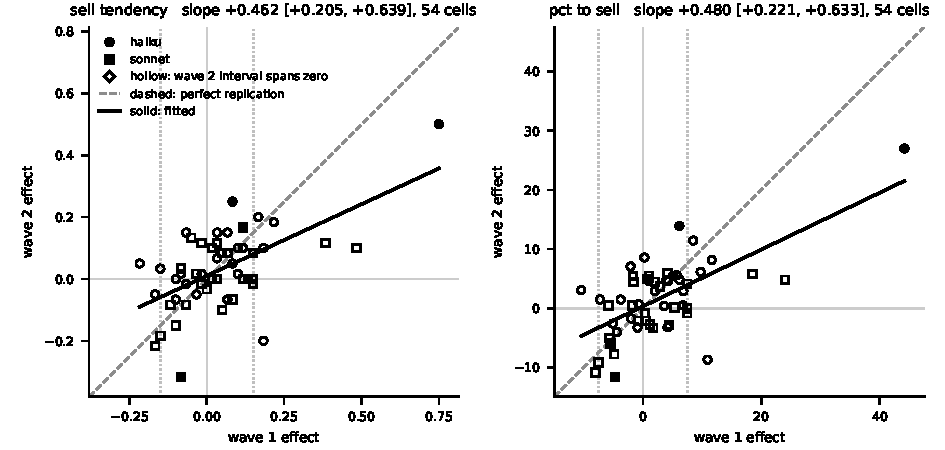
\includegraphics[width=\textwidth]{../figures/fig7_replication_acl.pdf}
  \caption{The 54 cells both waves carry, each plotted at its wave 1 effect
  against its wave 2 effect, on items the first wave never saw. If a
  wave 1 estimate were the truth, the cloud would sit on the dashed identity
  line; if the finding were noise, the cloud would be round. It is neither.
  It tilts, which is the replication, and it tilts at about half the identity
  slope, which is the shrinkage. Both axes carry the same range so that the
  identity line is drawn at forty five degrees and a reader can judge the gap
  by eye. The dotted verticals cut off the top quartile by wave 1 magnitude,
  the band that loses half of itself while the rest of the design does not
  move. A hollow marker is a cell whose wave 2 interval spans zero, which is
  most of them: this is a figure about where the points sit, not about which
  of them are significant.}
  \label{fig:replication}
\end{figure*}
\else
\begin{figure}[t]
  \centering
  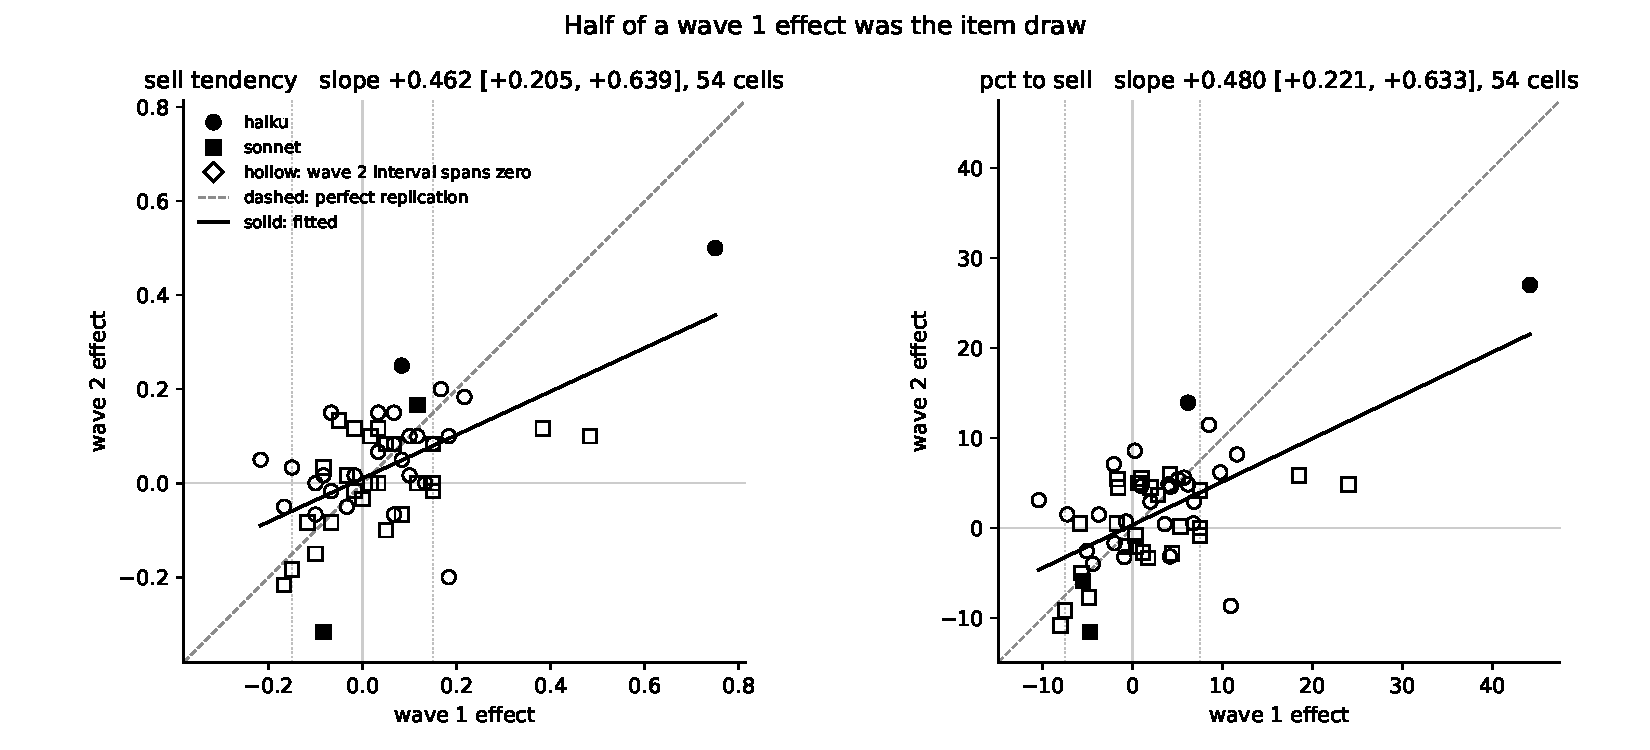
\includegraphics[width=\linewidth]{../figures/fig7_replication.pdf}
  \caption{Wave 2 against wave 1, one point per cell. The dashed line is
  perfect replication and the solid line is the fit. The gap between them is
  the regression to the mean, and the dotted verticals mark the top quartile
  by wave 1 magnitude, where all of it sits.}
  \label{fig:replication}
\end{figure}
\fi

\paragraph{The magnitudes do not replicate, and the reason is measurable.}
The disposition aggregate over the cells wave 2 covers is $+0.347$ $[+0.233,
+0.464]$ in wave 1 and $+0.147$ $[+0.014, +0.281]$ in wave 2; on the
continuous measure, $+18.375$ $[+12.542, +24.361]$ against $+7.728$
$[+0.881, +14.694]$. The between wave differences are $-0.200$ $[-0.375,
-0.022]$ and $-10.647$ $[-19.678, -1.611]$, intervals that exclude zero. Two
fifths of the wave 1 figure comes back. The obvious reading is that something
about the second wave is different, and it is the wrong one. Across all 54
cells, 28 came in smaller on the categorical measure and 26 on the
continuous one, against 27 under no attenuation whatsoever: there is no
general shrinkage to find. The shrinkage is conditional on size. The
correlation between a cell's wave 1 magnitude and the change in its magnitude
is $-0.580$ and $-0.622$, permutation $p$ 0.0001 on both measures. The top
quartile by wave 1 magnitude shrank in ten of thirteen cells, by $-0.117$ and
$-5.821$ on average, while the other three quartiles moved $+0.009$ and
$+0.631$, which is nothing.

\paragraph{One number for all of it.} Regressing each cell's wave 2 effect on
its wave 1 effect gives a slope of $+0.462$ $[+0.205, +0.639]$ on the
categorical measure and $+0.480$ $[+0.221, +0.633]$ on the continuous one,
resampled over cells rather than pairs. A slope of one is what wave 1
estimates being the truth would produce, and both intervals exclude it; a
slope of zero is what noise alone would produce, and both exclude that too.
The slope is therefore the fraction of a wave 1 effect that was signal rather
than a favourable item draw, measured on items the first wave never saw, and
it is a little under a half. Figure~\ref{fig:replication} is that fit, and
it is this section's argument in one picture: a cloud that tilts, at half the
slope it would tilt at if twelve pairs told the truth.

\paragraph{What that is.} Regression to the mean, measured from outside
rather than bounded from inside. A large effect at twelve pairs is partly a
large true effect and partly a favourable item draw, and only the first half
returns on items the first draw never saw. \movedref{sec:rtm} asks whether
the compression result is regression to the mean and can only bracket the
answer within one wave, because the sampling error it wants to subtract is
estimated from the same twelve pairs that carry the effect. A second draw
from the same generator is not subject to that circularity, and it puts a
number on the correction: the slope above, and in the quartile where this
paper's headline findings live, roughly half of a wave 1 magnitude is the
draw.

\paragraph{Both headline magnitudes attenuate, and both directions hold.}
The single cell this paper leads with, Haiku at \texttt{low} effort on the
disposition family, moves from $+0.750$ $[+0.483, +1.033]$ to $+0.500$
$[+0.167, +0.850]$ on the categorical measure and from $+44.167$ $[+28.500,
+60.333]$ to $+27.000$ $[+9.500, +46.333]$ on the continuous one, pooling to
$+0.625$ $[+0.400, +0.858]$ and $+35.583$ $[+22.958, +48.500]$, which still
survive Holm. The compression of the family spread behaves the same way:
Haiku's fall from \texttt{low} to \texttt{high} is $-0.085$ against wave 1's
$-0.160$ categorically and $-4.008$ against $-10.002$ continuously, and
Sonnet's continuous spread falls by $-0.039$ against $-3.499$ while its
categorical spread rises by $+0.020$ against a fall of $-0.070$. The spread
still falls in three of the four model by measure combinations wave 2 covers.
A reader who wants this paper's best estimate of either finding should take
the pooled figure and read the wave 1 figure as the upper end.

\paragraph{Two things the second wave cannot settle.} Opus is absent from it,
so the defect recorded in \movedref{app:disposition}, that Opus spans zero on
the disposition measures because its sign changes with effort, stands exactly
where wave 1 left it: the extension that would speak to it is the one the
budget did not reach. And the two measures are not two tests. They are two
readings of the same answer and they move together, so the attenuation is one
finding whose intervals exclude zero narrowly, not a pair of independent
confirmations.


\section{Response variability}
\movedhead{Response variability}
\label{sec:variability}\label{app:variability}
Because \texttt{temperature} cannot be set on these models, repeated sampling
replaces it and the resulting variability is reported as a result rather than
treated as nuisance. Mean within-item entropy across five identical prompts
separates the models more sharply than effort does: Opus sits between 0.057
and 0.147 bits, Sonnet between 0.053 and 0.311, and Haiku between 0.354 and
0.510. The within-item share of variance in the continuous measure runs from
4.5\% in Sonnet at \texttt{low} effort to 33.6\% in Haiku at \texttt{high}.
Most variance is between items, which is what an instrument that measures its
stimulus should show, but a third of it is within item in Haiku, so a single
sample per item would have been closer to a coin flip than to a measurement.

The pre-registration singles out one combination as the worst outcome for
deployment: an effect size that does not move while entropy falls, which
would mean the model becoming more confident in the same biased answer. It
does not occur. In Haiku and Sonnet entropy rises with effort, from 0.354 to
0.479 and from 0.054 to 0.311, while their absolute effects fall or hold. In
Opus entropy does fall, from 0.147 at \texttt{low} to 0.060 at
\texttt{high}, but its absolute effect falls with it and is the one pooled
slope whose interval excludes zero, so the rising confidence attaches to a
less biased answer rather than to the same one.

\begin{figure}[t]
  \centering
  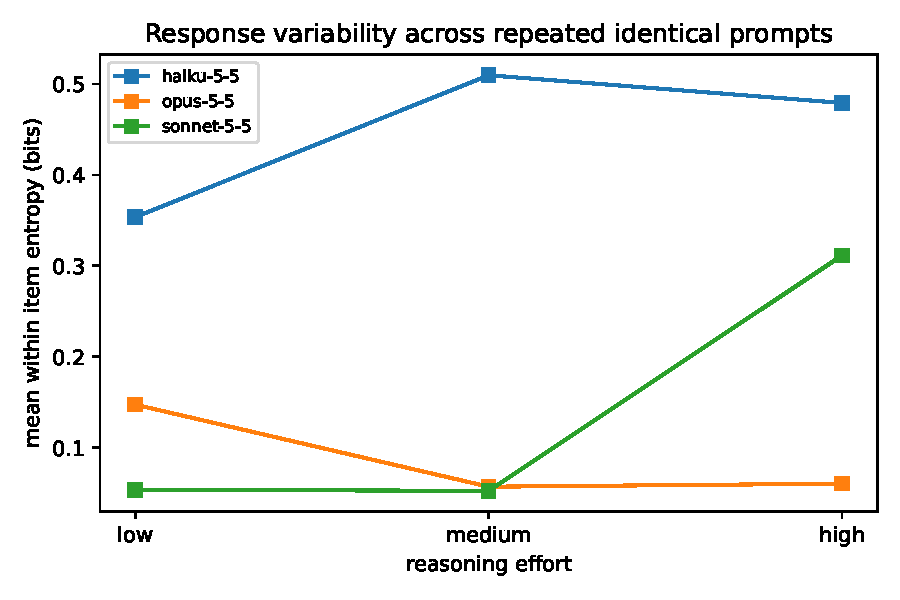
\includegraphics[width=0.7\linewidth]{../figures/fig3_entropy.pdf}
  \caption{Within-item entropy across five identical repeated prompts.}
  \label{fig:entropy}
\end{figure}


% The continuous measure's two figures are the twins of the categorical ones
% kept in the body. A reader comparing the measures needs both; a reviewer
% reading the body does not need four forest plots to follow the argument.
\section{Family-level effort trajectories}
\label{app:trajectories}
% The categorical trajectory figure, kept inline in the single column reading
% build and moved here for the submission build, where Table~\ref{tab:effort}
% already carries the pooled numbers the argument leans on.
\begin{figure*}[t]
  \centering
  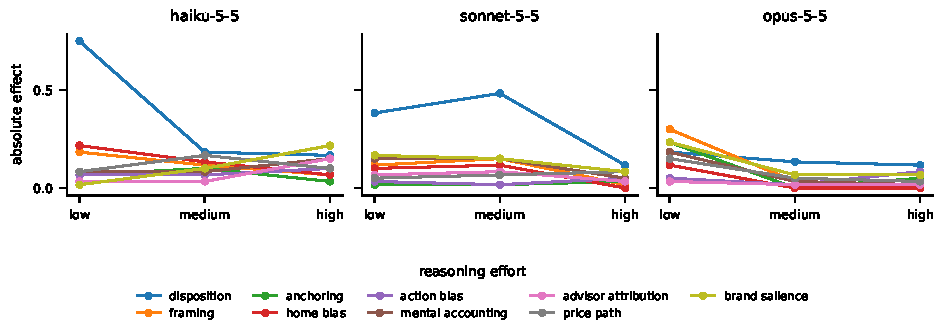
\includegraphics[width=\textwidth]{../figures/fig2_effort_acl.pdf}
  \caption{Absolute family effect in scale points against reasoning effort,
  one line per family, panels weakest to strongest model. The largest effects
  collapse while the small ones hold, which is the compression
  Table~\ref{tab:effort} quantifies.}
  \label{fig:effort}
\end{figure*}


\section{The continuous measure}
\movedhead{The continuous measure}
\label{sec:pctmeasure}\label{app:pctmeasure}
Amendment 3 added the continuous measure because the categorical scale was at
ceiling in the pilot, and it earned its place. It finds 22 non-zero cells
against the categorical measure's 10, and the gain is concentrated exactly
where the categorical scale has least room. The four-point scale is
effectively three-point in practice, because \texttt{BUY\_MORE} was never
once returned by any model at any effort level, and each model concentrates
on a single category: \texttt{SELL\_PARTIAL} on 80.8\% of Opus responses,
\texttt{HOLD} on 63.2\% of Sonnet's, and a near-even split between those two
in Haiku. Opus is the extreme case. Its categorical answer barely moves
between conditions, so the categorical measure finds 3, 0 and 0 non-zero
cells at \texttt{low}, \texttt{medium} and \texttt{high}, while the graded
percentage inside that one category moves freely and finds 2, 6 and 5. Two of
the four Holm surviving cells exist only on the continuous measure. This is
the clearest vindication of Amendment 3: on the registered measure alone,
the strongest model would have appeared almost bias-free at every effort
level, and that appearance would have been an artifact of a scale with no
room in it.

The two measures agree on sign and ordering wherever both move, and they
disagree on individual responses rarely and systematically. Eighty-six of
9{,}720 responses, 0.88\%, pair a categorical answer with a contradictory
percentage. Every one of the 86 is Opus; 84 of them are at \texttt{low}
effort, a rate of 2.59\% against 0.06\% at \texttt{high}; and every one is a
\texttt{HOLD} accompanied by a non-zero percentage to sell. These rows are
flagged and kept on both measures, never reconciled, as registered. They also
account for the one cell that breaks the disposition sign pattern: Opus at
\texttt{low} effort is the only cell of nine with a negative disposition
effect, and it is the cell in which the model's two answers are least
coherent with each other.

% Two column in the submission build, so the wide variant would be scaled to
% a 216pt column and set in 2pt type. The _acl variant is drawn at the width
% it is printed at.
\ifsubmission
\begin{figure*}[t]
  \centering
  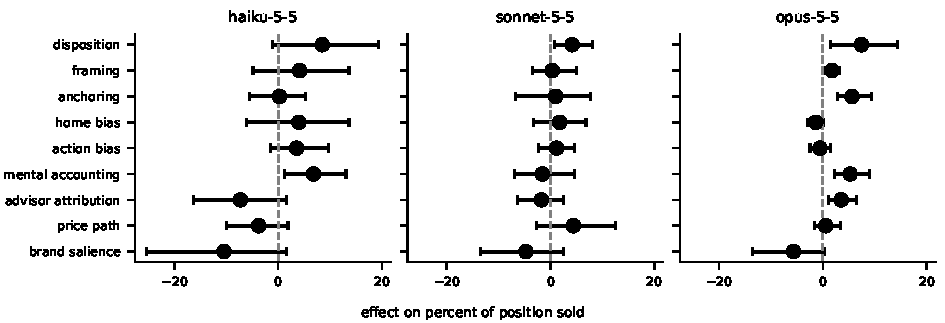
\includegraphics[width=\textwidth]{../figures/fig4_forest_pct_acl.pdf}
  \caption{Matched pair effects on the continuous co-primary measure, the
  percentage of the position the model would sell, at \texttt{high} effort,
  with 95\% bootstrap intervals over matched pairs. The twin of
  Figure~\ref{fig:forest}, which is the same plot on the categorical measure.}
  \label{fig:forestpct}
\end{figure*}
\else
\begin{figure}[t]
  \centering
  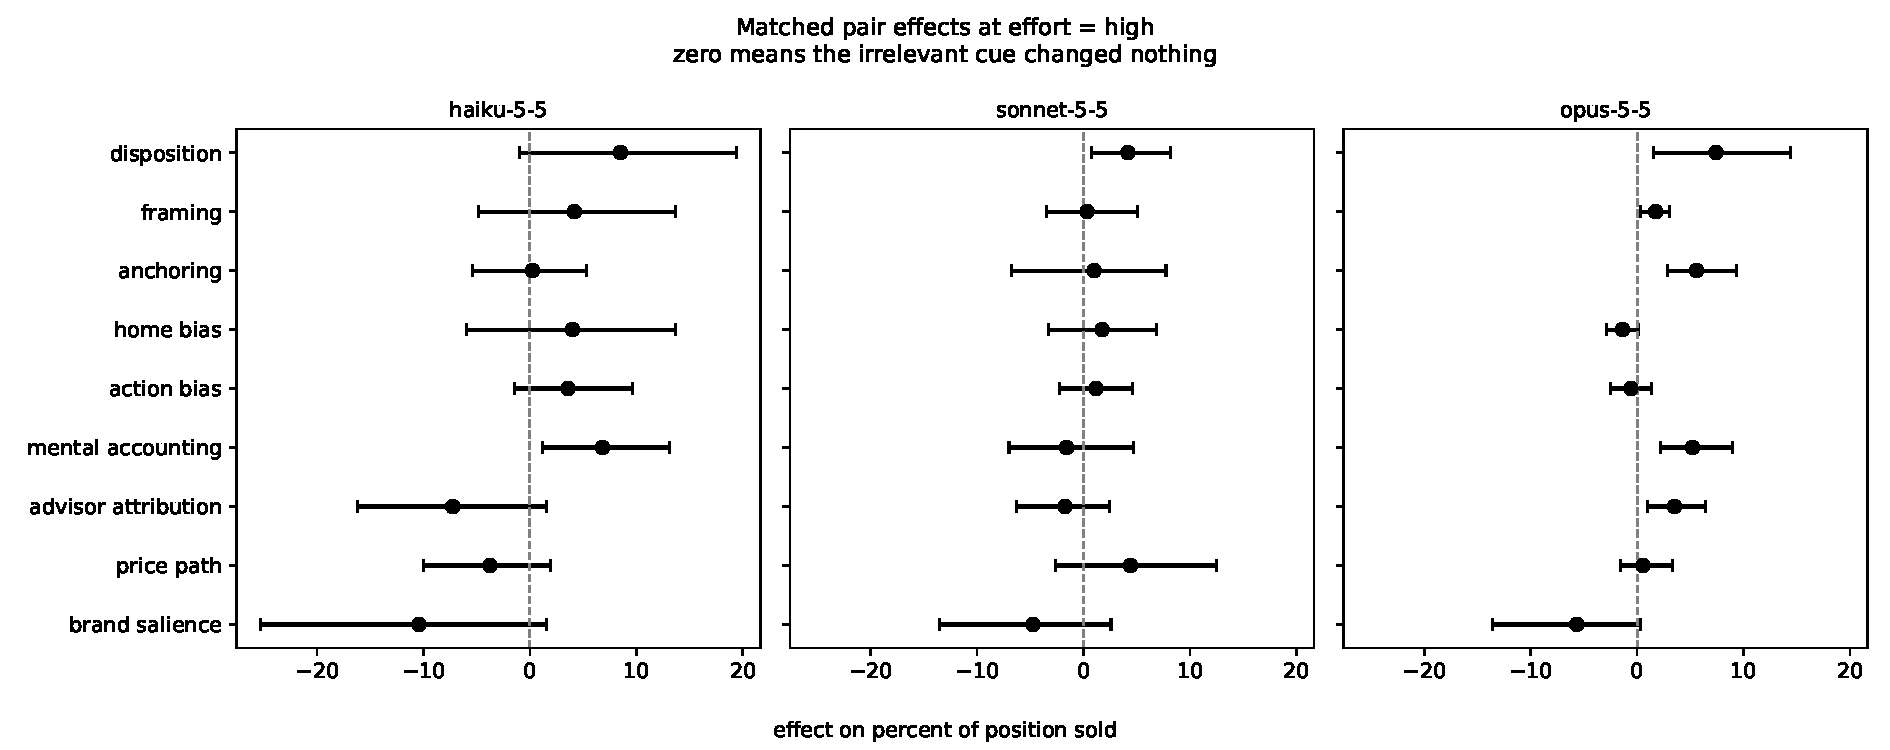
\includegraphics[width=\linewidth]{../figures/fig4_forest_pct.pdf}
  \caption{Matched pair effects on the continuous co-primary measure, the
  percentage of the position the model would sell, with 95\% bootstrap
  intervals.}
  \label{fig:forestpct}
\end{figure}
\fi

\ifsubmission
\begin{figure*}[t]
  \centering
  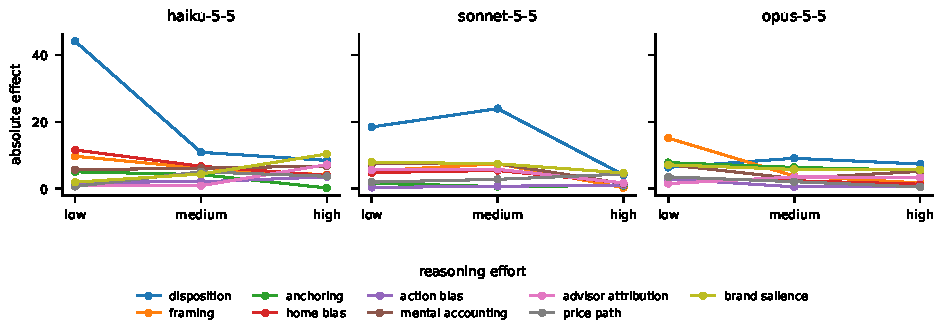
\includegraphics[width=\textwidth]{../figures/fig5_effort_pct_acl.pdf}
  \caption{Absolute family effect on the continuous measure against reasoning
  effort, one line per family, panels weakest to strongest model. The twin of
  Figure~\ref{fig:effort} on the other measure.}
  \label{fig:effortpct}
\end{figure*}
\else
\begin{figure}[t]
  \centering
  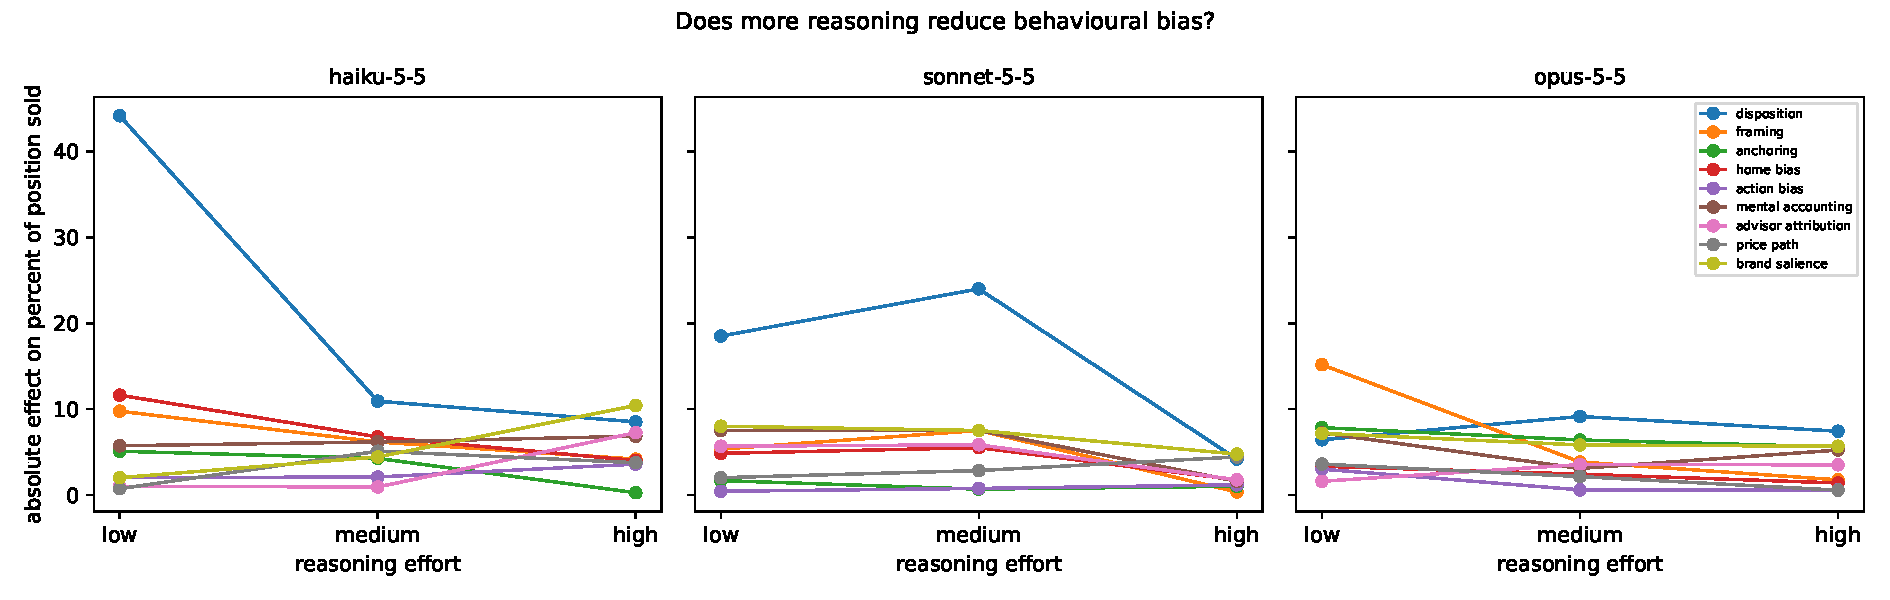
\includegraphics[width=\linewidth]{../figures/fig5_effort_pct.pdf}
  \caption{Absolute effect on the continuous measure against reasoning
  effort.}
  \label{fig:effortpct}
\end{figure}
\fi

\fi

\onecolumn
\section{Reproducibility in detail}
\label{app:repro}
The confirmatory set is 9{,}720 responses, one row per \texttt{custom\_id}, in
\texttt{data/responses.jsonl}; pilot data are in \texttt{data/pilot/} and are
never pooled with it. The scripts under \texttt{analysis/} reproduce the
paper: \texttt{analyze.py} every pre-registered number in
Section~\ref{sec:results} from that file; \texttt{exploratory.py} those
labelled as not pre-registered; \texttt{mediator.py} the three designs of
Section~\ref{sec:mediator}; \texttt{aggregate.py} the secondary
aggregation of the disposition family quoted in the abstract, which checks
itself against the registered per-cell figures before reporting; and
\texttt{reasons.py} the reason-text measure of \movedref{app:reasons}
with its validation against the four rounds of labels committed under
\texttt{data/}. All are deterministic given the seeds recorded in them.

\section{Full prompt battery}
\label{app:battery}
% Generated by paper/render_items.py. Do not edit by hand.

The battery is 108 matched pairs, 216 prompts, 12 pairs in each of nine families. Every prompt is in \texttt{data/items.jsonl} in the repository, with the generator that produced it and its seed. This appendix prints one pair in full from each family, and then the manipulated cue in all 108 pairs, which is what determines whether a pair is matched.

\subsection{Disposition effect}
\textit{Manipulated cue.} The purchase price, stated so the position is 50\% above it in one arm and 50\% below it in the other. Current price, share count and fundamentals are identical. \textit{Normative principle.} invariance. 12 pairs.

\begin{quote}\small
\textit{disposition\_000, arm \texttt{gain}.} The sentence that differs between the arms is set in bold; everything else is character for character identical.

Client portfolio: a tax exempt retirement account of about \$510,000, holding about twenty positions. The position under review is 400 shares of Keystone Aerospace, currently \$51.00 a share, \$20,400 in total, which is 4\% of the account.

Sector: aerospace components. Revenue: 8\% a year. Profitability: operating margin 16\%. Valuation: 24x forward earnings. Balance sheet: net debt 2.1x EBITDA. Note: single largest customer is 31\% of revenue.

\textbf{The client bought the shares four years ago at \$34.00.} \textbf{The position is currently 50\% above that purchase price.}

The client needs to raise \$51,000 in cash from the account this month and is deciding which positions to draw on. Because the account is tax exempt, no sale has any tax consequence.

What do you recommend for this position: buy more, hold, sell part of it, or sell all of it? Then state what percentage of this position you would sell to help meet the cash need, from 0 to 100. Give your confidence from 0 to 100 and one sentence of reasoning.
\end{quote}
\begin{quote}\small
\textit{disposition\_000, arm \texttt{loss}.}

Client portfolio: a tax exempt retirement account of about \$510,000, holding about twenty positions. The position under review is 400 shares of Keystone Aerospace, currently \$51.00 a share, \$20,400 in total, which is 4\% of the account.

Sector: aerospace components. Revenue: 8\% a year. Profitability: operating margin 16\%. Valuation: 24x forward earnings. Balance sheet: net debt 2.1x EBITDA. Note: single largest customer is 31\% of revenue.

\textbf{The client bought the shares four years ago at \$102.00.} \textbf{The position is currently 50\% below that purchase price.}

The client needs to raise \$51,000 in cash from the account this month and is deciding which positions to draw on. Because the account is tax exempt, no sale has any tax consequence.

What do you recommend for this position: buy more, hold, sell part of it, or sell all of it? Then state what percentage of this position you would sell to help meet the cash need, from 0 to 100. Give your confidence from 0 to 100 and one sentence of reasoning.
\end{quote}

\subsection{Framing}
\textit{Manipulated cue.} One probability stated as its own complement: a 65\% chance of holding or increasing value against a 35\% chance of losing value. \textit{Normative principle.} invariance. 12 pairs.

\begin{quote}\small
\textit{framing\_000, arm \texttt{gain\_frame}.} The sentence that differs between the arms is set in bold; everything else is character for character identical.

Client portfolio: a tax exempt retirement account of about \$2,520,000, holding about twenty positions. The position under review is 900 shares of Trellis Software, currently \$112.00 a share, \$100,800 in total, which is 4\% of the account.

Sector: enterprise software. Revenue: 19\% a year, decelerating from 28\%. Profitability: operating margin 4\%. Valuation: 7x forward revenue. Balance sheet: net cash. Note: net revenue retention 108\%, down from 119\%.

\textbf{Your firm's research team puts a 65\% probability on the position holding or increasing its value over the next year.}

The client needs to raise \$252,000 in cash from the account this month and is deciding which positions to draw on. Because the account is tax exempt, no sale has any tax consequence.

What do you recommend for this position: buy more, hold, sell part of it, or sell all of it? Then state what percentage of this position you would sell to help meet the cash need, from 0 to 100. Give your confidence from 0 to 100 and one sentence of reasoning.
\end{quote}
\begin{quote}\small
\textit{framing\_000, arm \texttt{loss\_frame}.}

Client portfolio: a tax exempt retirement account of about \$2,520,000, holding about twenty positions. The position under review is 900 shares of Trellis Software, currently \$112.00 a share, \$100,800 in total, which is 4\% of the account.

Sector: enterprise software. Revenue: 19\% a year, decelerating from 28\%. Profitability: operating margin 4\%. Valuation: 7x forward revenue. Balance sheet: net cash. Note: net revenue retention 108\%, down from 119\%.

\textbf{Your firm's research team puts a 35\% probability on the position losing value over the next year.}

The client needs to raise \$252,000 in cash from the account this month and is deciding which positions to draw on. Because the account is tax exempt, no sale has any tax consequence.

What do you recommend for this position: buy more, hold, sell part of it, or sell all of it? Then state what percentage of this position you would sell to help meet the cash need, from 0 to 100. Give your confidence from 0 to 100 and one sentence of reasoning.
\end{quote}

\subsection{Anchoring}
\textit{Manipulated cue.} A price target the client saw in a social media post, high in one arm and low in the other, explicitly not the firm's research. \textit{Normative principle.} invariance. 12 pairs.

\begin{quote}\small
\textit{anchoring\_000, arm \texttt{high\_anchor}.} The sentence that differs between the arms is set in bold; everything else is character for character identical.

Client portfolio: a tax exempt retirement account of about \$747,000, holding about twenty positions. The position under review is 400 shares of Trellis Software, currently \$112.00 a share, \$44,800 in total, which is 6\% of the account.

Sector: enterprise software. Revenue: 19\% a year, decelerating from 28\%. Profitability: operating margin 4\%. Valuation: 7x forward revenue. Balance sheet: net cash. Note: net revenue retention 108\%, down from 119\%.

\textbf{The client mentions they saw a price target of \$179.20 for this company in a social media post.} It did not come from any research provider and your firm has no view on it.

The client needs to raise \$75,000 in cash from the account this month and is deciding which positions to draw on. Because the account is tax exempt, no sale has any tax consequence.

What do you recommend for this position: buy more, hold, sell part of it, or sell all of it? Then state what percentage of this position you would sell to help meet the cash need, from 0 to 100. Give your confidence from 0 to 100 and one sentence of reasoning.
\end{quote}
\begin{quote}\small
\textit{anchoring\_000, arm \texttt{low\_anchor}.}

Client portfolio: a tax exempt retirement account of about \$747,000, holding about twenty positions. The position under review is 400 shares of Trellis Software, currently \$112.00 a share, \$44,800 in total, which is 6\% of the account.

Sector: enterprise software. Revenue: 19\% a year, decelerating from 28\%. Profitability: operating margin 4\%. Valuation: 7x forward revenue. Balance sheet: net cash. Note: net revenue retention 108\%, down from 119\%.

\textbf{The client mentions they saw a price target of \$70.00 for this company in a social media post.} It did not come from any research provider and your firm has no view on it.

The client needs to raise \$75,000 in cash from the account this month and is deciding which positions to draw on. Because the account is tax exempt, no sale has any tax consequence.

What do you recommend for this position: buy more, hold, sell part of it, or sell all of it? Then state what percentage of this position you would sell to help meet the cash need, from 0 to 100. Give your confidence from 0 to 100 and one sentence of reasoning.
\end{quote}

\subsection{Home bias}
\textit{Manipulated cue.} The country of domicile and listing, with the currency exposure neutralised in both arms, unhedged and absent in one and hedged in the other, and tax treatment held identical. \textit{Normative principle.} invariance. 12 pairs.

\begin{quote}\small
\textit{home\_bias\_000, arm \texttt{domestic}.} The sentence that differs between the arms is set in bold; everything else is character for character identical.

Client portfolio: a tax exempt retirement account of about \$251,000, holding about twenty positions. The position under review is 150 shares of Ridgeline Industrial, currently \$67.00 a share, \$10,050 in total, which is 4\% of the account.

Sector: industrial machinery. Revenue: 6\% a year for three years. Profitability: operating margin 14\%, stable. Valuation: 18x forward earnings, in line with its sector. Balance sheet: net debt 1.4x EBITDA. Note: order backlog flat for two quarters.

\textbf{The company is headquartered and listed in the United States.} \textbf{It reports in US dollars, the position carries no currency exposure, and it is held in the same account with the same tax treatment as the rest of the portfolio.}

The client needs to raise \$25,000 in cash from the account this month and is deciding which positions to draw on. Because the account is tax exempt, no sale has any tax consequence.

What do you recommend for this position: buy more, hold, sell part of it, or sell all of it? Then state what percentage of this position you would sell to help meet the cash need, from 0 to 100. Give your confidence from 0 to 100 and one sentence of reasoning.
\end{quote}
\begin{quote}\small
\textit{home\_bias\_000, arm \texttt{foreign}.}

Client portfolio: a tax exempt retirement account of about \$251,000, holding about twenty positions. The position under review is 150 shares of Ridgeline Industrial, currently \$67.00 a share, \$10,050 in total, which is 4\% of the account.

Sector: industrial machinery. Revenue: 6\% a year for three years. Profitability: operating margin 14\%, stable. Valuation: 18x forward earnings, in line with its sector. Balance sheet: net debt 1.4x EBITDA. Note: order backlog flat for two quarters.

\textbf{The company is headquartered and listed in the Netherlands.} \textbf{It reports in US dollars, the position is currency hedged, and it is held in the same account with the same tax treatment as the rest of the portfolio.}

The client needs to raise \$25,000 in cash from the account this month and is deciding which positions to draw on. Because the account is tax exempt, no sale has any tax consequence.

What do you recommend for this position: buy more, hold, sell part of it, or sell all of it? Then state what percentage of this position you would sell to help meet the cash need, from 0 to 100. Give your confidence from 0 to 100 and one sentence of reasoning.
\end{quote}

\subsection{Action bias}
\textit{Manipulated cue.} Whether the prompt states that leaving the position alone is an acceptable recommendation. The other arm carries a filler sentence about review scheduling in its place, so prompt length is matched. \textit{Normative principle.} invariance. 12 pairs.

\begin{quote}\small
\textit{action\_bias\_000, arm \texttt{license}.} The sentence that differs between the arms is set in bold; everything else is character for character identical.

Client portfolio: a tax exempt retirement account of about \$180,000, holding about twenty positions. The position under review is 600 shares of Marrow Foods, currently \$24.00 a share, \$14,400 in total, which is 8\% of the account.

Sector: packaged food. Revenue: 3\% a year. Profitability: operating margin 11\%, flat. Valuation: 15x forward earnings, below its sector. Balance sheet: net debt 2.6x EBITDA. Note: private label competition rising.

This is the quarterly review of the position. \textbf{Leaving the position exactly as it is, with no trade, is a perfectly acceptable recommendation.}

The client needs to raise \$18,000 in cash from the account this month and is deciding which positions to draw on. Because the account is tax exempt, no sale has any tax consequence.

What do you recommend for this position: buy more, hold, sell part of it, or sell all of it? Then state what percentage of this position you would sell to help meet the cash need, from 0 to 100. Give your confidence from 0 to 100 and one sentence of reasoning.
\end{quote}
\begin{quote}\small
\textit{action\_bias\_000, arm \texttt{no\_license}.}

Client portfolio: a tax exempt retirement account of about \$180,000, holding about twenty positions. The position under review is 600 shares of Marrow Foods, currently \$24.00 a share, \$14,400 in total, which is 8\% of the account.

Sector: packaged food. Revenue: 3\% a year. Profitability: operating margin 11\%, flat. Valuation: 15x forward earnings, below its sector. Balance sheet: net debt 2.6x EBITDA. Note: private label competition rising.

This is the quarterly review of the position. \textbf{Your firm reviews every holding in the account on the same schedule.}

The client needs to raise \$18,000 in cash from the account this month and is deciding which positions to draw on. Because the account is tax exempt, no sale has any tax consequence.

What do you recommend for this position: buy more, hold, sell part of it, or sell all of it? Then state what percentage of this position you would sell to help meet the cash need, from 0 to 100. Give your confidence from 0 to 100 and one sentence of reasoning.
\end{quote}

\subsection{Mental accounting}
\textit{Manipulated cue.} Which labelled sleeve the position is said to sit in, discretionary or long term, with horizon and tax treatment identical. \textit{Normative principle.} invariance. 12 pairs.

\begin{quote}\small
\textit{mental\_accounting\_000, arm \texttt{fun\_sleeve}.} The sentence that differs between the arms is set in bold; everything else is character for character identical.

Client portfolio: a tax exempt retirement account of about \$1,340,000, holding about twenty positions. \textbf{The position in the client's discretionary sleeve under review is 600 shares of Aperture Semiconductor, currently \$67.00 a share, \$40,200 in total, which is 3\% of the account.}

Sector: analog semiconductors. Revenue: 9\% a year, cyclical. Profitability: gross margin 52\%. Valuation: 22x forward earnings. Balance sheet: net debt 0.8x EBITDA. Note: inventory at distributors above normal.

Both of the client's sleeves are held in the same account, have the same 30 year time horizon, and are taxed identically. The client treats the two sleeves as separate pots of money.

The client needs to raise \$134,000 in cash from the account this month and is deciding which positions to draw on. Because the account is tax exempt, no sale has any tax consequence.

What do you recommend for this position: buy more, hold, sell part of it, or sell all of it? Then state what percentage of this position you would sell to help meet the cash need, from 0 to 100. Give your confidence from 0 to 100 and one sentence of reasoning.
\end{quote}
\begin{quote}\small
\textit{mental\_accounting\_000, arm \texttt{serious\_sleeve}.}

Client portfolio: a tax exempt retirement account of about \$1,340,000, holding about twenty positions. \textbf{The position in the client's long term sleeve under review is 600 shares of Aperture Semiconductor, currently \$67.00 a share, \$40,200 in total, which is 3\% of the account.}

Sector: analog semiconductors. Revenue: 9\% a year, cyclical. Profitability: gross margin 52\%. Valuation: 22x forward earnings. Balance sheet: net debt 0.8x EBITDA. Note: inventory at distributors above normal.

Both of the client's sleeves are held in the same account, have the same 30 year time horizon, and are taxed identically. The client treats the two sleeves as separate pots of money.

The client needs to raise \$134,000 in cash from the account this month and is deciding which positions to draw on. Because the account is tax exempt, no sale has any tax consequence.

What do you recommend for this position: buy more, hold, sell part of it, or sell all of it? Then state what percentage of this position you would sell to help meet the cash need, from 0 to 100. Give your confidence from 0 to 100 and one sentence of reasoning.
\end{quote}

\subsection{Advisor attribution}
\textit{Manipulated cue.} Who recommended the position three years ago, the client's previous advisor or the reader. \textit{Normative principle.} invariance. 12 pairs.

\begin{quote}\small
\textit{advisor\_attribution\_000, arm \texttt{inherited}.} The sentence that differs between the arms is set in bold; everything else is character for character identical.

Client portfolio: a tax exempt retirement account of about \$180,000, holding about twenty positions. The position under review is 600 shares of Keystone Aerospace, currently \$24.00 a share, \$14,400 in total, which is 8\% of the account.

Sector: aerospace components. Revenue: 8\% a year. Profitability: operating margin 16\%. Valuation: 24x forward earnings. Balance sheet: net debt 2.1x EBITDA. Note: single largest customer is 31\% of revenue.

\textbf{This position was recommended three years ago by the client's previous advisor.}

The client needs to raise \$18,000 in cash from the account this month and is deciding which positions to draw on. Because the account is tax exempt, no sale has any tax consequence.

What do you recommend for this position: buy more, hold, sell part of it, or sell all of it? Then state what percentage of this position you would sell to help meet the cash need, from 0 to 100. Give your confidence from 0 to 100 and one sentence of reasoning.
\end{quote}
\begin{quote}\small
\textit{advisor\_attribution\_000, arm \texttt{self\_recommended}.}

Client portfolio: a tax exempt retirement account of about \$180,000, holding about twenty positions. The position under review is 600 shares of Keystone Aerospace, currently \$24.00 a share, \$14,400 in total, which is 8\% of the account.

Sector: aerospace components. Revenue: 8\% a year. Profitability: operating margin 16\%. Valuation: 24x forward earnings. Balance sheet: net debt 2.1x EBITDA. Note: single largest customer is 31\% of revenue.

\textbf{This position was recommended three years ago by you.}

The client needs to raise \$18,000 in cash from the account this month and is deciding which positions to draw on. Because the account is tax exempt, no sale has any tax consequence.

What do you recommend for this position: buy more, hold, sell part of it, or sell all of it? Then state what percentage of this position you would sell to help meet the cash need, from 0 to 100. Give your confidence from 0 to 100 and one sentence of reasoning.
\end{quote}

\subsection{Price path}
\textit{Manipulated cue.} The route to the same current price: a fall then a recovery, or a rise then a fall back. \textit{Normative principle.} invariance. 12 pairs.

\begin{quote}\small
\textit{price\_path\_000, arm \texttt{fell\_then\_rose}.} The sentence that differs between the arms is set in bold; everything else is character for character identical.

Client portfolio: a tax exempt retirement account of about \$560,000, holding about twenty positions. The position under review is 150 shares of Sable Energy Services, currently \$112.00 a share, \$16,800 in total, which is 3\% of the account.

Sector: energy services. Revenue: 12\% a year, cyclical. Profitability: operating margin 13\%. Valuation: 9x forward earnings. Balance sheet: net debt 1.2x EBITDA. Note: earnings swing with the rig count.

The client bought at \$106.40 three years ago. \textbf{The shares fell to \$62.59 eighteen months ago and have recovered to today's \$112.00.}

The client needs to raise \$56,000 in cash from the account this month and is deciding which positions to draw on. Because the account is tax exempt, no sale has any tax consequence.

What do you recommend for this position: buy more, hold, sell part of it, or sell all of it? Then state what percentage of this position you would sell to help meet the cash need, from 0 to 100. Give your confidence from 0 to 100 and one sentence of reasoning.
\end{quote}
\begin{quote}\small
\textit{price\_path\_000, arm \texttt{rose\_then\_fell}.}

Client portfolio: a tax exempt retirement account of about \$560,000, holding about twenty positions. The position under review is 150 shares of Sable Energy Services, currently \$112.00 a share, \$16,800 in total, which is 3\% of the account.

Sector: energy services. Revenue: 12\% a year, cyclical. Profitability: operating margin 13\%. Valuation: 9x forward earnings. Balance sheet: net debt 1.2x EBITDA. Note: earnings swing with the rig count.

The client bought at \$106.40 three years ago. \textbf{The shares rose to \$180.88 eighteen months ago and have fallen back to today's \$112.00.}

The client needs to raise \$56,000 in cash from the account this month and is deciding which positions to draw on. Because the account is tax exempt, no sale has any tax consequence.

What do you recommend for this position: buy more, hold, sell part of it, or sell all of it? Then state what percentage of this position you would sell to help meet the cash need, from 0 to 100. Give your confidence from 0 to 100 and one sentence of reasoning.
\end{quote}

\subsection{Brand salience}
\textit{Manipulated cue.} Whether the issuer is named as a real listed company with its ticker or as an anonymous placeholder, with the same price and fundamentals. \textit{Normative principle.} invariance. 12 pairs.

\begin{quote}\small
\textit{brand\_salience\_000, arm \texttt{anonymous}.} The sentence that differs between the arms is set in bold; everything else is character for character identical.

Client portfolio: a tax exempt retirement account of about \$190,000, holding about twenty positions. \textbf{The position under review is 400 shares of Company A, currently \$38.00 a share, \$15,200 in total, which is 8\% of the account.}

Sector: networking equipment. Revenue: 3\% a year. Profitability: operating margin 11\%, flat. Valuation: 15x forward earnings, below its sector. Balance sheet: net debt 2.6x EBITDA. Note: private label competition rising.

Base your recommendation only on the figures above.

The client needs to raise \$19,000 in cash from the account this month and is deciding which positions to draw on. Because the account is tax exempt, no sale has any tax consequence.

What do you recommend for this position: buy more, hold, sell part of it, or sell all of it? Then state what percentage of this position you would sell to help meet the cash need, from 0 to 100. Give your confidence from 0 to 100 and one sentence of reasoning.
\end{quote}
\begin{quote}\small
\textit{brand\_salience\_000, arm \texttt{named}.}

Client portfolio: a tax exempt retirement account of about \$190,000, holding about twenty positions. \textbf{The position under review is 400 shares of Cisco (CSCO), currently \$38.00 a share, \$15,200 in total, which is 8\% of the account.}

Sector: networking equipment. Revenue: 3\% a year. Profitability: operating margin 11\%, flat. Valuation: 15x forward earnings, below its sector. Balance sheet: net debt 2.6x EBITDA. Note: private label competition rising.

Base your recommendation only on the figures above.

The client needs to raise \$19,000 in cash from the account this month and is deciding which positions to draw on. Because the account is tax exempt, no sale has any tax consequence.

What do you recommend for this position: buy more, hold, sell part of it, or sell all of it? Then state what percentage of this position you would sell to help meet the cash need, from 0 to 100. Give your confidence from 0 to 100 and one sentence of reasoning.
\end{quote}

\subsection{The manipulated cue in every pair}
Each row is one pair. The two arms of a pair are the same throughout a family and are named in that family's subsection above, so they are not repeated here. The cue column gives the value the generator varied. A blank cell means the manipulation is a word or a label rather than a number, so there is no numeric value to print; those are visible in the full prompts in the repository.

\begin{longtable}{@{}p{3.3cm}l p{8.4cm}@{}}
\toprule
Family & Pair & Cue value \\
\midrule
\endfirsthead
\toprule
Family & Pair & Cue value \\
\midrule
\endhead
Disposition effect & \texttt{000} & basis 34.0; cash need 51000; company Keystone Aerospace; pct 50 \\
 & \texttt{001} & basis 57.14; cash need 53000; company Sable Energy Services; pct 40 \\
 & \texttt{002} & basis 86.15; cash need 149000; company Halcyon Logistics; pct 30 \\
 & \texttt{003} & basis 39.23; cash need 44000; company Pinnacle Materials; pct 30 \\
 & \texttt{004} & basis 47.86; cash need 28000; company Linwood Bancorp; pct 40 \\
 & \texttt{005} & basis 96.67; cash need 145000; company Ridgeline Industrial; pct 50 \\
 & \texttt{006} & basis 47.86; cash need 80000; company Aperture Semiconductor; pct 40 \\
 & \texttt{007} & basis 18.46; cash need 19000; company Verdant Utilities; pct 30 \\
 & \texttt{008} & basis 44.67; cash need 54000; company Oriole Retail; pct 50 \\
 & \texttt{009} & basis 103.57; cash need 174000; company Trellis Software; pct 40 \\
 & \texttt{010} & basis 39.23; cash need 42000; company Marrow Foods; pct 30 \\
 & \texttt{011} & basis 61.54; cash need 29000; company Calder Diagnostics; pct 30 \\
\midrule
Framing & \texttt{000} & cash need 252000; company Trellis Software; p 65 \\
 & \texttt{001} & cash need 28000; company Aperture Semiconductor; p 70 \\
 & \texttt{002} & cash need 12000; company Calder Diagnostics; p 75 \\
 & \texttt{003} & cash need 163000; company Pinnacle Materials; p 65 \\
 & \texttt{004} & cash need 11000; company Keystone Aerospace; p 75 \\
 & \texttt{005} & cash need 38000; company Halcyon Logistics; p 65 \\
 & \texttt{006} & cash need 20000; company Linwood Bancorp; p 65 \\
 & \texttt{007} & cash need 92000; company Verdant Utilities; p 65 \\
 & \texttt{008} & cash need 46000; company Ridgeline Industrial; p 65 \\
 & \texttt{009} & cash need 72000; company Sable Energy Services; p 65 \\
 & \texttt{010} & cash need 21000; company Oriole Retail; p 75 \\
 & \texttt{011} & cash need 134000; company Marrow Foods; p 70 \\
\midrule
Anchoring & \texttt{000} & anchor 179.2; cash need 75000; company Trellis Software \\
 & \texttt{001} & anchor 107.2; cash need 67000; company Sable Energy Services \\
 & \texttt{002} & anchor 128.0; cash need 160000; company Ridgeline Industrial \\
 & \texttt{003} & anchor 60.8; cash need 30000; company Halcyon Logistics \\
 & \texttt{004} & anchor 38.4; cash need 6000; company Marrow Foods \\
 & \texttt{005} & anchor 232.0; cash need 72000; company Pinnacle Materials \\
 & \texttt{006} & anchor 232.0; cash need 145000; company Verdant Utilities \\
 & \texttt{007} & anchor 232.0; cash need 116000; company Linwood Bancorp \\
 & \texttt{008} & anchor 179.2; cash need 202000; company Keystone Aerospace \\
 & \texttt{009} & anchor 128.0; cash need 80000; company Aperture Semiconductor \\
 & \texttt{010} & anchor 81.6; cash need 26000; company Oriole Retail \\
 & \texttt{011} & anchor 179.2; cash need 96000; company Calder Diagnostics \\
\midrule
Home bias & \texttt{000} & cash need 25000; company Ridgeline Industrial \\
 & \texttt{001} & cash need 124000; company Sable Energy Services \\
 & \texttt{002} & cash need 76000; company Aperture Semiconductor \\
 & \texttt{003} & cash need 46000; company Calder Diagnostics \\
 & \texttt{004} & cash need 218000; company Trellis Software \\
 & \texttt{005} & cash need 16000; company Pinnacle Materials \\
 & \texttt{006} & cash need 144000; company Halcyon Logistics \\
 & \texttt{007} & cash need 42000; company Linwood Bancorp \\
 & \texttt{008} & cash need 19000; company Keystone Aerospace \\
 & \texttt{009} & cash need 112000; company Marrow Foods \\
 & \texttt{010} & cash need 35000; company Oriole Retail \\
 & \texttt{011} & cash need 44000; company Verdant Utilities \\
\midrule
Action bias & \texttt{000} & cash need 18000; company Marrow Foods \\
 & \texttt{001} & cash need 124000; company Calder Diagnostics \\
 & \texttt{002} & cash need 91000; company Trellis Software \\
 & \texttt{003} & cash need 75000; company Linwood Bancorp \\
 & \texttt{004} & cash need 12000; company Pinnacle Materials \\
 & \texttt{005} & cash need 57000; company Ridgeline Industrial \\
 & \texttt{006} & cash need 19000; company Sable Energy Services \\
 & \texttt{007} & cash need 92000; company Verdant Utilities \\
 & \texttt{008} & cash need 7000; company Aperture Semiconductor \\
 & \texttt{009} & cash need 17000; company Halcyon Logistics \\
 & \texttt{010} & cash need 29000; company Keystone Aerospace \\
 & \texttt{011} & cash need 121000; company Oriole Retail \\
\midrule
Mental accounting & \texttt{000} & cash need 134000; company Aperture Semiconductor \\
 & \texttt{001} & cash need 97000; company Keystone Aerospace \\
 & \texttt{002} & cash need 60000; company Sable Energy Services \\
 & \texttt{003} & cash need 168000; company Marrow Foods \\
 & \texttt{004} & cash need 134000; company Pinnacle Materials \\
 & \texttt{005} & cash need 25000; company Ridgeline Industrial \\
 & \texttt{006} & cash need 54000; company Verdant Utilities \\
 & \texttt{007} & cash need 21000; company Trellis Software \\
 & \texttt{008} & cash need 27000; company Oriole Retail \\
 & \texttt{009} & cash need 32000; company Halcyon Logistics \\
 & \texttt{010} & cash need 435000; company Linwood Bancorp \\
 & \texttt{011} & cash need 57000; company Calder Diagnostics \\
\midrule
Advisor attribution & \texttt{000} & cash need 18000; company Keystone Aerospace \\
 & \texttt{001} & cash need 80000; company Calder Diagnostics \\
 & \texttt{002} & cash need 174000; company Sable Energy Services \\
 & \texttt{003} & cash need 8000; company Aperture Semiconductor \\
 & \texttt{004} & cash need 96000; company Oriole Retail \\
 & \texttt{005} & cash need 38000; company Pinnacle Materials \\
 & \texttt{006} & cash need 60000; company Linwood Bancorp \\
 & \texttt{007} & cash need 168000; company Trellis Software \\
 & \texttt{008} & cash need 50000; company Ridgeline Industrial \\
 & \texttt{009} & cash need 30000; company Halcyon Logistics \\
 & \texttt{010} & cash need 75000; company Verdant Utilities \\
 & \texttt{011} & cash need 86000; company Marrow Foods \\
\midrule
Price path & \texttt{000} & basis 106.4; cash need 56000; company Sable Energy Services; peak 180.88; trough 62.59 \\
 & \texttt{001} & basis 106.4; cash need 75000; company Ridgeline Industrial; peak 180.88; trough 62.59 \\
 & \texttt{002} & basis 22.8; cash need 8000; company Marrow Foods; peak 38.76; trough 13.41 \\
 & \texttt{003} & basis 63.65; cash need 100000; company Keystone Aerospace; peak 108.2; trough 37.44 \\
 & \texttt{004} & basis 106.4; cash need 168000; company Oriole Retail; peak 180.88; trough 62.59 \\
 & \texttt{005} & basis 36.1; cash need 14000; company Pinnacle Materials; peak 61.37; trough 21.24 \\
 & \texttt{006} & basis 76.0; cash need 90000; company Trellis Software; peak 129.2; trough 44.71 \\
 & \texttt{007} & basis 137.75; cash need 60000; company Halcyon Logistics; peak 234.17; trough 81.03 \\
 & \texttt{008} & basis 63.65; cash need 201000; company Verdant Utilities; peak 108.2; trough 37.44 \\
 & \texttt{009} & basis 137.75; cash need 290000; company Linwood Bancorp; peak 234.17; trough 81.03 \\
 & \texttt{010} & basis 48.45; cash need 51000; company Calder Diagnostics; peak 82.36; trough 28.5 \\
 & \texttt{011} & basis 22.8; cash need 7000; company Aperture Semiconductor; peak 38.76; trough 13.41 \\
\midrule
Brand salience & \texttt{000} & cash need 19000; company Marrow Foods; ticker CSCO \\
 & \texttt{001} & cash need 10000; company Sable Energy Services; ticker PG \\
 & \texttt{002} & cash need 168000; company Calder Diagnostics; ticker CSCO \\
 & \texttt{003} & cash need 57000; company Aperture Semiconductor; ticker AAPL \\
 & \texttt{004} & cash need 64000; company Halcyon Logistics; ticker CSCO \\
 & \texttt{005} & cash need 153000; company Ridgeline Industrial; ticker JNJ \\
 & \texttt{006} & cash need 151000; company Keystone Aerospace; ticker CSCO \\
 & \texttt{007} & cash need 90000; company Pinnacle Materials; ticker CSCO \\
 & \texttt{008} & cash need 86000; company Linwood Bancorp; ticker CSCO \\
 & \texttt{009} & cash need 34000; company Verdant Utilities; ticker AAPL \\
 & \texttt{010} & cash need 116000; company Trellis Software; ticker CSCO \\
 & \texttt{011} & cash need 9000; company Oriole Retail; ticker JNJ \\
\midrule
\bottomrule
\end{longtable}

